%% !TeX program = LuaLaTeX
%% !TeX encoding = UTF-8

%----------------------------------------------------------------------------------------
%	PACKAGES AND OTHER DOCUMENT CONFIGURATIONS
%----------------------------------------------------------------------------------------
%\UseRawInputEncoding
%\DeclareUnicodeCharacter{00A0}{~}
\documentclass[ 
11pt, % The default document font size, options: 10pt, 11pt, 12pt
% oneside, % Two side (alternating margins) for binding by default, uncomment to switch to one side
french, % ngerman for German
singlespacing, % Single line spacing, alternatives: onehalfspacing or doublespacing
% draft, % Uncomment to enable draft mode (no pictures, no links, overfull hboxes indicated)
%nolistspacing, % If the document is onehalfspacing or doublespacing, uncomment this to set spacing in lists to single
% liststotoc, % Uncomment to add the list of figures/tables/etc to the table of contents
%toctotoc, % Uncomment to add the main table of contents to the table of contents
parskip, % Uncomment to add space between paragraphs
%nohyperref, % Uncomment to not load the hyperref package
headsepline, % Uncomment to get a line under the header
%chapterinoneline, % Uncomment to place the chapter title next to the number on one line
%consistentlayout, % Uncomment to change the layout of the declaration, abstract and acknowledgements pages to match the default layout
openany, %% Use this option to make chapters start on the next page, irrespective of whether it's an odd or even numbered page
]{MastersDoctoralThesis} % The class file specifying the document structure


%%-----------------------
% \usepackage{mathpazo} % Use the Palatino font by default
% \usepackage[charter]{mathdesign}
%%-----------------------
% \usepackage[partialup,lighttext]{kpfonts}        %% For math only
% \usepackage{fontspec}       %% Because we are using XeTEX
% \setromanfont{Minion Pro}   %% For text (Minion Math is commercial)
% \setsansfont{Fira Sans Light}
%%-----------------------
\usepackage[utf8]{inputenc} % Required for inputting international characters
\usepackage[T1]{fontenc} % Output font encoding for international characters
\usepackage{textcomp}
\usepackage[lf]{venturis}
\usepackage{libertinust1math}
%%-----------------------

\usepackage{sectsty}        %% Pour mettre les titres en Sans Serif
\allsectionsfont{\sffamily}

% \setcounter{tocdepth}{4} %% Use this to set numbering depth for sections in the toc (already set in the Class)
\setcounter{secnumdepth}{3} %% Use this to set numbering depth for sections in the whole document

\graphicspath{ {./Figures/} } %% To load all images in this document from the Figures directory
\DeclareGraphicsExtensions{.pdf,.png}  %% Use to this to set the priority for extensions leading
\usepackage{caption}
\captionsetup{font={footnotesize}, textfont={sf}, labelfont={bf,sf}}
\usepackage[font=sf]{floatrow}  %% For other floet content
% \captionsetup[figure]{font=it}
\usepackage{subcaption} %% Use to make subgraphics
\usepackage{float} %% Use this to control where the images are placed compared to thier related text
\usepackage{multirow}
\usepackage{listings}

\usepackage{tikz}
\usetikzlibrary{patterns}
\usepackage{tikzscale}

\usepackage{amsthm}
\usepackage{amsmath,bm,mathtools} %% Use this to include the "align" environment in witch equations can be made easier
\usepackage{physics} %% To have physical terms like the divergence operator
\usepackage{cases}  %% For the numcases environnment

%\usepackage[backend=bibtex,style=numeric,maxnames=2,natbib=true]{biblatex} % Use the bibtex backend with the numeric citation style
\usepackage[backend=bibtex,style=alphabetic,maxnames=2,natbib=true]{biblatex} % Use the bibtex backend with the authoryear citation style (which resembles APA)
% \bibliographystyle{abbrv}
%\usepackage[backend=bibtex,style=authoryear-comp,sorting=none,sortcites=true,doi=false,url=false,giveninits=true,hyperref]{biblatex}

\addbibresource{bibliography.bib} % The filename of the bibliography
\addbibresource{bibliography_matthias.bib} % The filename of the bibliography
\addbibresource{bibliography_dimitri.bib} % The filename of the bibliography

\usepackage[autostyle=true]{csquotes} % Required to generate language-dependent quotes in the bibliography 

\usepackage{indentfirst}  %% For indentation

\usepackage{xcolor}   %% To add color to text

\usepackage{hyperref}
\usepackage{cleveref} %% To reference stuf
\usepackage{upgreek}
\usepackage{amsfonts}
%\usepackage{psnfss}
%\usepackage{psnfss}
%\usepackage{psnfss}

% \usepackage{multline}

%----------------------------------------------------------------------------------------

\renewcommand{\emph}[1]{\textbf{\textit{#1}}} %% Use this to make \emph text bold (you lose all other properties of the command)

\newcommand{\Run}{\mathbb{R}}
\newcommand{\Rdeux}{\mathbb{R}^2}
\newcommand{\Rtrois}{\mathbb{R}^3}
\newcommand{\hplus}{h_{+}}
\newcommand{\hmoins}{h_{-}}
\newcommand{\eun}{\bvec{e}_1(\omega)}
\newcommand{\edeux}{\bvec{e}_2(\omega)}

\newcommand{\bvec}[1]{\bm{\mathrm{#1}}}  %% Use this to make vectors
\newcommand{\bmat}[1]{\bm{\mathsf{#1}}}   %% Use this to make tensors

\newcommand{\R}{\mathcal{R}}
\renewcommand{\P}{\mathcal{P}}

\newcommand{\diff}{\,\differential}
\newcommand{\intO}[1]{\int_{\Omega^{#1}(t)}}
\newcommand{\dtstar}{\delta t^*}

\newcommand{\identity}{\text{Id}}

\newcommand{\eel}{E_{\text{ \upshape el}}}
\newcommand{\efrac}{E_{\text{\upshape frac}}}
\newcommand{\etot}{E_{\text{\upshape tot}}}
\newcommand{\wadm}{W_{\text{\upshape adm}}}

\newcommand{\tmoins}{t^{-}}
\newcommand{\tplus}{t^{+}}
\newcommand{\tdelta}{\delta t^{*}}

\newtheorem{theorem}{Theorème}
\numberwithin{theorem}{section}  %% Pour numeroter par section
\newtheorem{corollary}[theorem]{Corollaire}

\NewDocumentCommand{\myfig}{ O{99} O{fig:latest} m m}{
  \begin{figure}       
    \frame{\includegraphics[width=.#1\textwidth]{#3}}       
    \caption{#4.}
    \label{fig:#2}
  \end{figure}
}

\newcommand{\myvec}[2]{\begin{pmatrix} #1  \\ #2 \end{pmatrix}}   %% vecteur 2d
\newcommand{\mymat}[4]{\begin{pmatrix} #1 & #2 \\ #3 & #4 \end{pmatrix}}  %% Matrice 2*2

\newcommand{\mybigvec}[3]{\begin{pmatrix} #1  \\ #2 \\ #3 \end{pmatrix}}   %% vecteur 3d
\newcommand{\mybigmat}[9]{\begin{pmatrix} #1 & #2  & #3 \\ #4 & #5 & #6 \\ #7 & #8 & #9 \end{pmatrix}}  %% Matrice 3*3

%----------------------------------------------------------------------------------------
%	MARGIN SETTINGS
%----------------------------------------------------------------------------------------

%% To have a uniform margin on all pages
\geometry{
	paper=a4paper, % Change to letterpaper for US letter
	inner=0.75in, % Inner margin
	outer=0.75in, % Outer margin
	bindingoffset=.5cm, % Binding offset
	top=1.5cm, % Top margin
	bottom=1.5cm, % Bottom margin
	%showframe, % Uncomment to show how the type block is set on the page
}

%----------------------------------------------------------------------------------------
%	THESIS INFORMATION
%----------------------------------------------------------------------------------------

\thesistitle{\sffamily Fracturation de floes de glace par percussion \\dans un modèle granulaire} % Your thesis title, ths is used in the title and abstract, print it elsewhere with \ttitle
\supervisor{\href{https://www-ljk.imag.fr/membres/Stephane.Labbe/}{Stéphane \textsc{Labbé}}} % Your supervisor's name, this is used in the title page, print it elsewhere with \supname
\examiner{Christophe \textsc{Prud'homme}} % Your examiner's name, this is not currently used anywhere in the template, print it elsewhere with \examname
% \degree{master 2 CSMI} % Your degree name, this is used in the title page and abstract, print it elsewhere with \degreename
\author{Roussel Desmond \textsc{Nzoyem}} % Your name, this is used in the title page and abstract, print it elsewhere with \authorname
\addresses{} % Your address, this is not currently used anywhere in the template, print it elsewhere with \addressname

\subject{Mathématiques appliquées} % Your subject area, this is not currently used anywhere in the template, print it elsewhere with \subjectname
\keywords{} % Keywords for your thesis, this is not currently used anywhere in the template, print it elsewhere with \keywordnames
\university{\href{http://www.unistra.fr}{University of Strasbourg, Sorbonne Unisersité}} % Your university's name and URL, this is used in the title page and abstract, print it elsewhere with \univname
\department{\href{https://mathinfo.unistra.fr/}{UFR de mathématiques et d'informatique}} % Your department's name and URL, this is used in the title page and abstract, print it elsewhere with \deptname
\group{\href{https://mimesis.inria.fr/}{SASIP}} % Your research group's name and URL, this is used in the title page, print it elsewhere with \groupname
\faculty{\href{https://mathinfo.unistra.fr/}{UFR de mathématiques et d'informatique}} % Your faculty's name and URL, this is used in the title page and abstract, print it elsewhere with \facname

\AtBeginDocument{
\hypersetup{pdftitle=\ttitle} % Set the PDF's title to your title
\hypersetup{pdfauthor=\authorname} % Set the PDF's author to your name
\hypersetup{pdfkeywords=\keywordnames} % Set the PDF's keywords to your keywords
}


%\pdfmapfile{=/var/lib/texmf/fonts/map/pdftex/updmap/pdftex.map}

\begin{document}

\frontmatter % Use roman page numbering style (i, ii, iii, iv...) for the pre-content pages

\pagestyle{plain} % Default to the plain heading style until the thesis style is called for the body content

%----------------------------------------------------------------------------------------
%	TITLE PAGE
%----------------------------------------------------------------------------------------

\begin{titlepage}

\begin{figure}[!htb]
   \begin{minipage}{0.24\textwidth}
     \centering
     \vspace*{12pt}
     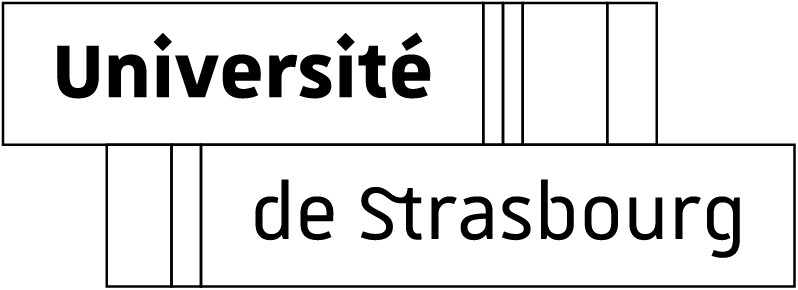
\includegraphics[width=.99\linewidth]{LogoUnistra2.png}
   \end{minipage}\hspace*{7pt}
   \begin{minipage}{0.24\textwidth}
    \centering
    
\includegraphics[width=.99\linewidth]{LogoCSMI.png}
  \end{minipage}\hfill
   \begin{minipage}{0.24\textwidth}
     \centering
     
\includegraphics[width=.6\linewidth]{LogoLJLL.jpg}
   \end{minipage}
   \begin{minipage}{0.24\textwidth}
    \centering
    
\includegraphics[width=.99\linewidth]{LogoSorbonne.png}
  \end{minipage}
\end{figure}


\begin{center}

\vspace*{.04\textheight}
% {\scshape\LARGE \univname\par}\vspace{1.5cm} % University name
\textsc{\Large Rapport de stage}\\[0.5cm] % Thesis type

\HRule \\[0.4cm] % Horizontal line
{\huge \bfseries \ttitle\par}\vspace{0.4cm} % Thesis title
\HRule \\[1.5cm] % Horizontal line

\begin{minipage}[t]{0.4\textwidth}
\begin{flushleft} \large
\vspace{7mm}
\emph{Étudiant}\\
\href{https://github.com/desmond-rn}{\authorname} % Author name - remove the \href bracket to remove the link
\end{flushleft}
\end{minipage}
\begin{minipage}[t]{0.4\textwidth}
\begin{flushright} \large
\emph{Superviseur} \\
\href{https://www-ljk.imag.fr/membres/Stephane.Labbe/}{\supname} % Supervisor names - remove the \href bracket to remove the link
\\ \vspace{5mm}
\emph{Enseignant référent} \\
\href{http://www.feelpp.org/team/prudhomm/}{\examname} % Examiner's name - remove the \href bracket to remove the link
\end{flushright}
\end{minipage}%%\\[2cm]

% \vfill

\begin{figure}[H]
    \centering
    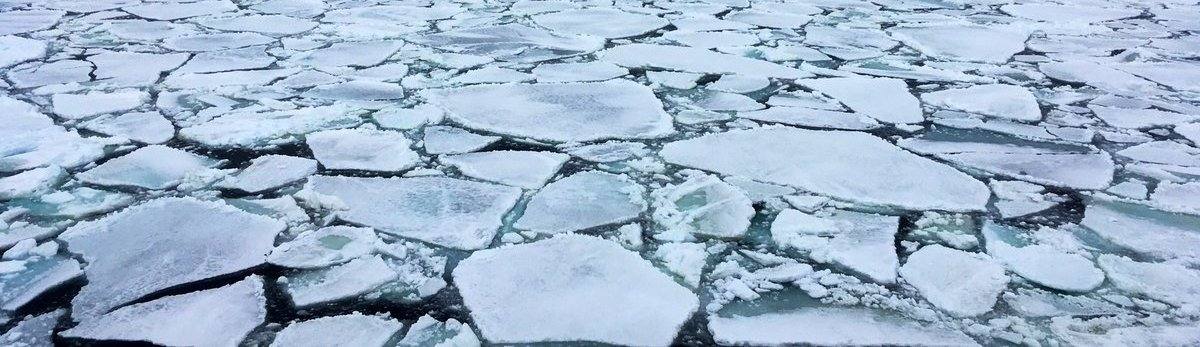
\includegraphics[width=.9\linewidth]{IntroPic.jpg}
    \label{Fig:IntroPic}
\end{figure}


% \large \textit{Ce stage à été effectué dans le cadre du \href{https://docs.google.com/document/d/10JbbXeqqu5J2BjMkSQRNQ8Gx7xBPOClLKpvd7EBZT8U/edit}{master 2 CSMI,}}\\[0.2cm]
% \textit{du 03 février 2021, au 31 juillet 2021;}\\[0.2cm]
% \textit{initié par le groupe \groupname \hspace*{1pt} au \href{https://www.ljll.math.upmc.fr/?lang=fr}{LJLL}.}\\[0.2cm]

\large \textit{Stage effectué au \href{https://www.ljll.math.upmc.fr/?lang=fr}{Laboratoire Jacques-Louis Lions};}\\[0.2cm]
\textit{du 03 février 2021, au 31 juillet 2021;}\\[0.2cm]
\textit{pour l'obtention du \href{https://docs.google.com/document/d/10JbbXeqqu5J2BjMkSQRNQ8Gx7xBPOClLKpvd7EBZT8U/edit}{master 2 CSMI}. }\\[0.2cm]

\vspace*{.04\textheight}
\large Année académique 2020 - 2021

\vfill

{\large \today}\\[4cm] % Today's date
% \includegraphics{Logo_UNIV} % University/department logo - uncomment to place it

% \vfill
\end{center}
\end{titlepage}

%----------------------------------------------------------------------------------------
%	DECLARATION PAGE
%----------------------------------------------------------------------------------------
%
% \begin{declaration}  
% \addchaptertocentry{\authorshipname} % Add the declaration to the table of contents
% \not I, \authorname, declare that this thesis titled, \enquote{\ttitle} and the work presented in it are my own. I confirm that:
%
% \begin{itemize}
% \item This work was done wholly or mainly while in candidature for a research degree at this University.
% \item Where any part of this thesis has previously been submitted for a degree or any other qualification at this University or any other institution, this has been clearly stated.
% \item Where I have consulted the published work of others, this is always clearly attributed.
% \item Where I have quoted from the work of others, the source is always given. With the exception of such quotations, this thesis is entirely my own work.
% \item I have acknowledged all main sources of help.
% \item Where the thesis is based on work done by myself jointly with others, I have made clear exactly what was done by others and what I have contributed myself.\\
% \end{itemize}
%
% \noindent Signed:\\
% \rule[0.5em]{25em}{0.5pt} % This prints a line for the signature
%
% \noindent Date:\\
% \rule[0.5em]{25em}{0.5pt} % This prints a line to write the date
% \end{declaration}
%
% \cleardoublepage

%----------------------------------------------------------------------------------------
%	QUOTATION PAGE
%----------------------------------------------------------------------------------------
%
% \vspace*{0.2\textheight}
%
% \noindent\enquote{\itshape Thanks to my solid academic training, today I can write hundreds of words on virtually any topic without possessing a shred of information, which is how I got a good job in journalism.}\bigbreak
%
% \hfill Dave Barry

%----------------------------------------------------------------------------------------
%	ABSTRACT PAGE
%----------------------------------------------------------------------------------------
%
% \begin{abstract}
% \addchaptertocentry{\abstractname} % Add the abstract to the table of contents
% The Thesis Abstract is written here (and usually kept to just this page). The page is kept centered vertically so can expand into the blank space above the title too\ldots
% \end{abstract}

% ----------------------------------------------------------------------------------------
% 	ACKNOWLEDGEMENTS
% ----------------------------------------------------------------------------------------

\begin{acknowledgements}
\addchaptertocentry{\acknowledgementname} % Add the acknowledgements to the table of contents

% Avant tout développement sur cette expérience professionnelle, il apparaît opportun de commencer ce rapport de stage par des remerciements, à ceux qui m’ont beaucoup appris au cours de ce stage, et même à ceux qui ont eu la gentillesse de faire de ce stage un moment très profitable.

% Aussi, je remercie \ldots, mon maître de stage qui m’a formé et accompagné tout au long de cette expérience professionnelle avec beaucoup de patience et de pédagogie. Enfin, je remercie l’ensemble des employés de \ldots pour les conseils qu’ils ont pu me prodiguer au cours de ces deux mois.

\end{acknowledgements}

%----------------------------------------------------------------------------------------
%	LIST OF CONTENTS/FIGURES/TABLES PAGES
%----------------------------------------------------------------------------------------

\tableofcontents % Prints the main table of contents

% \listoffigures % Prints the list of figures

% \listoftables % Prints the list of tables

%----------------------------------------------------------------------------------------
%	ABBREVIATIONS
%----------------------------------------------------------------------------------------

% \begin{abbreviations}{11} % Include a list of abbreviations (a table of two columns)
% 
% \addchaptertocentry{\abbreviations} % Add the abbreviations to the table of contents
% \textbf{ETR} & \textbf{E}quation (du) \textbf{T}ransfert \textbf{R}adiatif\\
% \textbf{ETL} & \textbf{E}quilibre \textbf{T}hermique \textbf{L}ocal\\
% \textbf{UFR} & \textbf{U}nite de\textbf{F}ormation et de \textbf{R}echerche de l'Universite de Strasbourg
% 
% \end{abbreviations}

%----------------------------------------------------------------------------------------
%	PHYSICAL CONSTANTS/OTHER DEFINITIONS
%----------------------------------------------------------------------------------------

% \begin{constants}{lr@{${}={}$}l} % The list of physical constants is a three column table
% 
% The \SI{}{} command is provided by the siunitx package, see its documentation for instructions on how to use it
% 
% Speed of Light & $c_{0}$ & \SI{2.99792458e8}{\meter\per\second} (exact)\\
% Constant Name & $Symbol$ & $Constant Value$ with units\\

% \end{constants}

%----------------------------------------------------------------------------------------
%	SYMBOLS
%----------------------------------------------------------------------------------------

% \begin{symbols}{rcc} % Include a list of Symbols (a three column table)
% \label{sec:symbols}
% \textbf{Symbole} & \textbf{Définition} & \textbf{Unité} \\
% \addlinespace % Gap to separate the Roman symbols from the Greek

% $x$ & Abscisse & \si{\cm} \\
% $y$ & Ordonnée & \si{\cm} \\
% $\bvec{x}$ & Vecteur position & \si{\cm} \\
% $\bm{\Omega}$ & Vecteur direction de propagation des photons & \si{\cm^2 \per \cm^2} \\
% $\nu$ & Fréquence & \si{Hz} \\
% $p$ & Fonction de distribution angulaire de « scattering » &  \\
% $I$ & Intensité spécifique de radiation & \si{W \per m^2 \per sr  \per Hz} \\
% $B$ & Fonction de Planck & \si{W \per m^2 \per sr  \per Hz} \\

% \addlinespace % Gap with real SI dimensions

% $\rho$ & Densité du milieu & \si{\g \per \cm\cubed} \\
% $\sigma_a$ & Opacité d'absorption & \si{\per\cm} \\
% $\sigma_c$ & Opacité de « scattering » (ou de dispersion) & \si{\per\cm} \\

% \addlinespace % Gap to separate inputs

% $t$ & Temps & \si{sh} \\
% $C_v$ & Capacité thermique du milieu & \si{Jerk \per\g \per keV} \\
% $a$ & Constante radiative (ou de rayonnement)& \si{g \per cm \per sh^2  \per keV } \\
% $c$ & Vitesse de la lumière & \si{\cm \per sh} \\

% \addlinespace % Gap to separate output

% $T$ & Température matière & \si{keV} \\
% $E$ & Energie des photons & \si{g \per \cm \per sh^2} \\
% $\bvec{F}$ & Flux de photons & \si{g \per sh^2} \\

% \end{symbols}

%----------------------------------------------------------------------------------------
%	DEDICATION
%----------------------------------------------------------------------------------------

% \dedicatory{For/Dedicated to/To my\ldots}

%----------------------------------------------------------------------------------------
%	THESIS CONTENT - CHAPTERS
%----------------------------------------------------------------------------------------

\mainmatter % Begin numeric (1,2,3...) page numbering
\setlength{\parindent}{4ex} %% Set the paragraph indentation as from this line

\pagestyle{thesis} % Return the page headers back to the "thesis" style

% Include the chapters of the thesis as separate files from the Chapters folder
% Uncomment the lines as you write the chapters

% % Chapter 1

\chapter{Introduction} % Main chapter title

\label{Chapter1} % For referencing the chapter elsewhere, use \ref{Chapter1} 

%----------------------------------------------------------------------------------------

% Define some commands to keep the formatting separated from the content 
\newcommand{\keyword}[1]{\textbf{#1}}
\newcommand{\tabhead}[1]{\textbf{#1}}
\newcommand{\code}[1]{\texttt{#1}}
\newcommand{\file}[1]{\texttt{\bfseries#1}}
\newcommand{\option}[1]{\texttt{\itshape#1}}






%1----------------------------------------------------------------------------------------



\section{Contexte}



Le déclin de la glace Artique ces dernières décenies est considéré comme l'une manifestations les plus marquante du changement climatique (voir \parencite{stroeve2012trends}). Ce déclin présente des enjeux aussi climatiques qu'industriels. Premièrement, de par son étendue et son epaisseur immense, la la zone artique est un contributeur majeur climat à travers ses échanges de chaleurs par rayonnement et radiation avec l'atmosphère. Il est donc crucial de considérer l'évolution de la glace dans les modèles climatiques. Deuxièmement, la chute de cette couverture de glace dans la MIZ\footnote{Marginal Ice Zone : zone de transition entre l’océan et le coeur de la banquise, où la concentration de
glace est inférieure à 80\%, et/ou les morceaux de glace sont de faible épaisseur ($\approx 1 mètre$) et de petite taille ($10 m - 100 km$).} (VOIR FIGURE) ouvre des routes maritimes facilitant l'exploitation de ses réserves d’hydrocarbures (qui restent quasiment intactes). Il est donc nécéssaire de pouvoir prédire l'évolution de la banquise Artique (au moins) à court terme.


Parmis les élément exhaxerbant ce déclin de galce Artique, des études ont cité l'accélération de la vitesse et de la déformation des floes\footnote{Un floe est un morceau indiviiduel de glace rencontré dans la MIZ} (RWDC11, SKM11). Pour les prédiction de l'évolution de la banquise, les modèles qui considère la glace comme un milieu continu ne sont pas adapté, surtout à l'échelle de la MIZ. Au contraire, les modèle granulaire, bien que plus couteux doivent etre priviligé afin de prendre en compte la nature discontinue de la banquise et sa rhéologie\footnote{étudie la résistance des matériaux aux contraintes et aux déformations.}. Des modèles granulaires pour l'évolution de la glace par le passé (Hop96, KS14). Cependant, les approches utulisées dans ces travaux limitent la géométrie (circulaire, rectangulaire) et le nombre de floes (de l'ordre de la centaine) (voir \parencite[p.16]{balasoiu2020halthesis}).


SASIP 



%2----------------------------------------------------------------------------------------





\section{Problématique et missions}








%3----------------------------------------------------------------------------------------





\section{Environnement}

LJLL, GRENOBLE et Teletravail





%4----------------------------------------------------------------------------------------





\section{Roadmap}
Missions (objectifs primaire) et secondaires. Ensuite les milestones. Enfin annonce du plan (qui résument les travaux)




% \subsection{Objectifs}
% INDIQUER ICI QUE LES TRAVAUX SERONT PRÉSENTÉS EN DETAILS DANS LES SECTIONS 2, 3, ET 4.









% \subsection{Les missions du poste}


% %%------------------- Cette partie doit etre intégrée à la suivante
% Au vue du problème qu'il nous est donné de résoudre et des travaux qui ont précédés, les taches suivantes (classées par ordre de priorité) ont été effectuées durant ce stage :

% \begin{enumerate}
%     \item Lecture des travaux de Dimitri et Matthias (des petits résumés)
%     \item Modéliser, simuler, etc..
%     \item Débugger et améliorer l'interface web de Dimitri:
%     \begin{itemize}
%         \item Correction du "collapsing" du Displacement Field
%         \item Correction du slider pour changer les images d'eigen vecteurs
%     \end{itemize}
% \end{enumerate}
% %%-------------------------- Citer ces taches sous forme de paragraphe LateX




% \begin{itemize}
%     \item L'état de l'art de la partie précédente fait partie des missions.
%     \item Modélisation
%     \item Simulation
% \end{itemize}

% Nous souhaitons étudier le comportement mécanique d'un floe après collision avec un autre floe. Les étapes de travail envisagées sont les suivantes:
% \begin{enumerate}
%     \item Ecire les systèmes differentiels pour les deux floes juste après le choc: pour l' instant on peut considérer que l'un des floes est immobile (celà revient au même si l'on exprimes les vitesses dans un repère lié à ce floe).
%     \item On exprime l'EDO vérifiée par les solutions, c'est à dire $q$ pour le premier floes, et $p$ pour le second.
%     \item On pourra ensuite simuler ces EDP limites et trouver les valeurs de $p$ et $q$. Autrement dit, on connait la position de chaque point du réseau au temps final.
%     \item Si on connait $p$ et/ou $q$, on connait la condition de Dirichlet sur le floe concerné, et on peut ainsi exprimer le déplacement et la possible fracture du floe. 
% \end{enumerate}






%5----------------------------------------------------------------------------------------




\section{Résumé de l'introduction en Anglais}       %% Introduction
% 
% Chapter 2

\chapter{État de l'art} % 3rd chapter title

\label{Chapter2} % For referencing the chapter elsewhere, use \ref{Chapter3} 

%%1----------------------------------------------------------------------------------------









 \section{Position du problème}
 \label{sec:position}


 Nous commençons par présenter une modélisation mathématique d'une plaque de glace (appelé floe) sur la mer. Six variables (locales) sont nécessaires pour décrire le floe occupant la région fermée de l'espace $\Omega$ (voir \cref{fig:floe}) :
 \begin{itemize}
     \item Un ouvert connexe $\omega \in \Rdeux$ décrivant la section longitudinale du floe ;
     \item Deux fonctions $\hplus, \hmoins \in \mathcal{F}(\omega, \Run)$ décrivant l'épaisseur du floe, telle que $\forall x \in \omega, \hmoins(x) \leq \hplus(x)$ ;
     \item Le centre de masse du floe $G(w)$ ;
     \item Deux vecteurs $\eun$ et $\edeux$ formant une base sur $\omega$.
 \end{itemize}

\begin{figure}[!ht]
     \centering
     \begin{subfigure}[b]{0.35\textwidth}
         \centering
         % 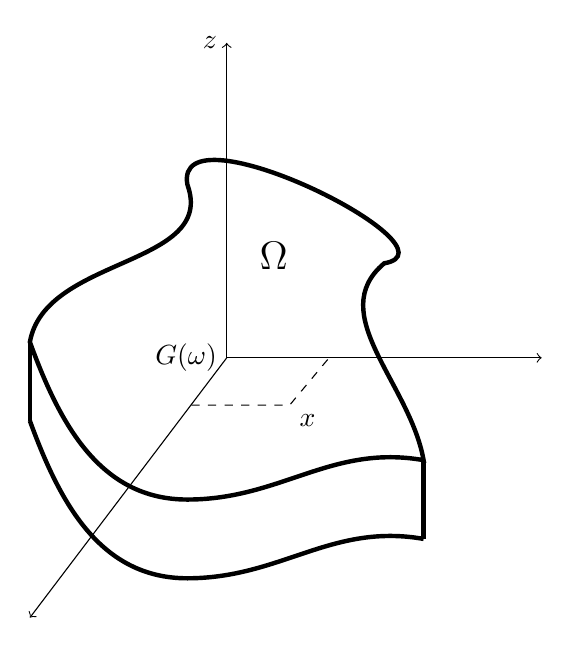
\begin{tikzpicture}
\node[coordinate] (v1) at (-3,3) {};
\node[coordinate] (v2) at (-5,1) {};
\node[coordinate] (v3) at (-3,-1) {};
\node[coordinate] (v4) at (0,-0.5) {};
\node[coordinate] (v5) at (-0.5,2) {};
%\draw  plot[smooth cycle, tension=.7] coordinates {(v5) (v1) (v2) (v3) (v4) (v5)};

\draw [ultra thick] (v1) to [out=290, in=80] (v2) to[out=290, in=180] (v3) to[out=0,in=170] (v4) to[out=100,in=220] (v5) to[out=10,in=100] (v1);

\node[coordinate] (v6) at (-5,0) {};
\node[coordinate] (v7) at (-3,-2) {};
\node[coordinate] (v8) at (0,-1.5) {};

\draw [ultra thick] (v2)--(v6); \draw [ultra thick] (v4)--(v8);
\draw [ultra thick]  (v6) to[out=290, in=180] (v7) to[out=0,in=170] (v8);

\node[coordinate] (v9) at (-2.5,0.8) {};
\node[coordinate] (v10) at (-5.0,-2.5) {};
\node[coordinate] (v11) at (1.5,0.8) {};
\node[coordinate] (v12) at (-2.5,4.8) {};

\draw [->] (v9)--(v10);
\draw [->] (v9)--(v11);
\draw [->] (v9)--(v12);


\node[left] (v9) at (-2.5,0.8) {$G(\omega)$};
\node[left] (v12) at (-2.5,4.8) {$z$};
\node[above left] (v13) at (-1.6,1.8) {\Large $\Omega$};

\node[coordinate] (v14) at (-1.2,0.8) {};
\node[coordinate] (v15) at (-1.7,0.2) {};
\node[coordinate] (v16) at (-2.95,0.2) {};
\draw[dashed] (v16)--(v15)--(v14);

\node[below right] (v15) at (-1.7,0.2) {$x$};

\end{tikzpicture}
         \includegraphics[width=.8\textwidth]{FloeVue1.tikz} 
         \caption{Vue d'un floe}
         \label{fig:floe1}
     \end{subfigure}
     % \hfill
     \begin{subfigure}[b]{0.35\textwidth}
         \centering
         % \usetikzlibrary{patterns}

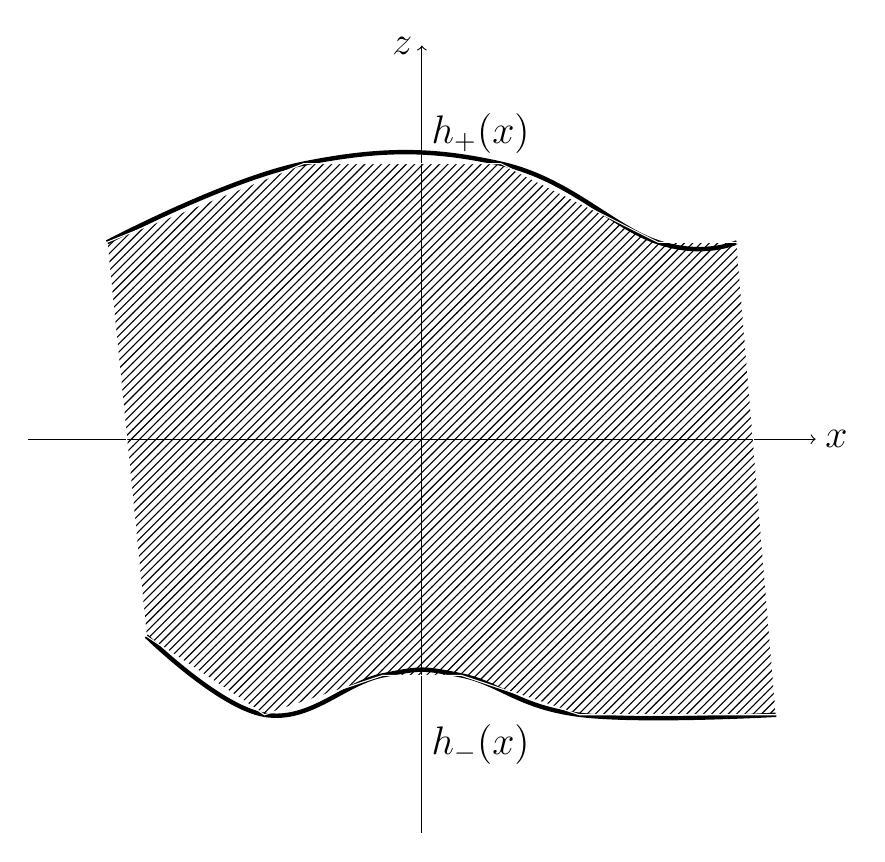
\begin{tikzpicture}

\node[coordinate] (v0) at (0,0) {};
\node[coordinate] (v1) at (-5,0) {};
\node[coordinate] (v2) at (5,0) {};
\node[coordinate] (v3) at (0,-5) {};
\node[coordinate] (v4) at (0,5) {};

\draw [->] (v1)--(v2);
\draw [->] (v3)--(v4);

\node (v5) at (-4,2.5) {};
\node (v6) at (-1.5,3.5) {};
\node (v7) at (1,3.5) {};
\node (v8) at (3,2.5) {};
\node (v9) at (4,2.5) {};
\node (v10) at (-3.5,-2.5) {};
\node (v11) at (-2,-3.5) {};
\node (v12) at (-0.5,-3) {};
\node (v13) at (0.5,-3) {};
\node (v14) at (2,-3.5) {};
\node (v15) at (4.5,-3.5) {};

\draw[ultra thick]  plot[smooth, tension=.7] coordinates {(v5) (v6) (v7) (v8) (v9)};
\draw[ultra thick]  plot[smooth, tension=.7] coordinates {(v10) (v11) (v12) (v13) (v14) (v15)};

\draw [white, pattern=north east lines, xshift=0.5cm,yshift=4.5cm] plot coordinates {(v5) (v6) (v7) (v8) (v9) (v15) (v14) (v13) (v12) (v11) (v10) (v5)};

\node [above right] at (0,3.5) {\Large \bfseries $h_{+}(x)$};
\node [below right] at (0,-3.5) {\Large \bfseries $h_{-}(x)$};
\node [right] at (5,0) {\Large \bfseries $x$};
\node [left] at (0,5) {\Large \bfseries $z$};

\end{tikzpicture} 
         \includegraphics[width=.8\textwidth]{FloeVue2.tikz} 
         % \includegraphics[width=2cm]{Figures/FloeVue2.tex}
         \caption{Coupe transversale}
         \label{fig:floe2}
     \end{subfigure}
        \caption{Illustration de la géométrie d'un floe de glace $\Omega$.}
        \label{fig:floe}
 \end{figure}

\noindent On confond le floe au volume qu'il occupe dans l'espace $\Omega$ :
 \[
     \Omega = \{(x,z) \,|\, x \in \omega \in \Rdeux, \, z \in \,]\hmoins(x), \hplus(x)[ \, \} \,.
 \] 
 Les fonctions $\hmoins$ et $\hplus$ permettent de définir trois quantités (voir \cref{fig:h}) :
 \begin{itemize}
     \item L'épaisseur moyenne du floe : $\bar{h} =  \sup_{x\in\omega}{\hplus(x)} - \inf_{x\in\omega}{\hmoins(x)}$ ;
     \item La plus forte épaisseur : $\bar{h}^* = \sup_{x\in\omega}{ \vert \hplus(x) - \hmoins(x) \vert}$ ;
     \item La plus faible épaisseur : $\underline{h}^* = \inf_{x\in\omega}{ \vert \hplus(x) - \hmoins(x) \vert}$. 
 \end{itemize}

\begin{figure}[!ht]
     \centering
     % \begin{tikzpicture}
	\begin{pgfonlayer}{nodelayer}
		\node [style=none] (0) at (0, 0) {};
		\node [style=none] (1) at (0, 5) {};
		\node [style=none] (2) at (0, -5) {};
		\node [style=none] (3) at (10, 0) {};
		\node [style=none] (4) at (-10, 0) {};
		\node [style=none] (5) at (-9.25, 2.5) {};
		\node [style=none] (6) at (-3.5, 1.5) {};
		\node [style=none] (7) at (3.25, 1.25) {};
		\node [style=none] (8) at (8.75, 4.75) {};
		\node [style=none] (9) at (-9, -6.75) {};
		\node [style=none] (10) at (-5, -4) {};
		\node [style=none] (11) at (2.5, -1.75) {};
		\node [style=none] (12) at (8.75, -1.25) {};
	\end{pgfonlayer}
	\begin{pgfonlayer}{edgelayer}
		\draw [->] (1.center) to (2.center);
		\draw [->] (4.center) to (3.center);
		\draw [bend right=15, looseness=0.75] (5.center) to (6.center);
		\draw [in=-165, out=0, looseness=1.25] (6.center) to (7.center);
		\draw [in=-135, out=15, looseness=1.25] (7.center) to (8.center);
		\draw [in=-165, out=45] (9.center) to (10.center);
		\draw [in=195, out=0, looseness=0.50] (10.center) to (11.center);
		\draw [in=180, out=15, looseness=0.75] (11.center) to (12.center);
	\end{pgfonlayer}
\end{tikzpicture}

     \includegraphics[width=.6\textwidth]{h.tikz}
     \caption{Différentes épaisseurs décrivant un floe de glace. Pour l'instant, afin d'obtenir un floe relativement plat (i.e. $\bar{h}$ faible), $\hmoins (\cdot)$ sera pris identiquement nul, et $\hplus (\cdot)$ constant.}
     \label{fig:h}
 \end{figure}

\noindent Les vecteurs $\eun$ et $\edeux$ sont liés à $\omega$, et pointent vers un point fixe du bord $\partial \omega$ du floe c-à-d :
 \[
     \exists \sigma_i \in \partial \omega \, | \, e_i(\omega) = \frac{\sigma_i - G(\omega)}{\Vert \sigma_i - G(\omega) \Vert}, \text{ pour } i \in \{1,2\} \,,
 \]
 où $\Vert \cdot \Vert$ désigne la norme euclidienne de $\Rdeux$. Notons que $\sigma_1 \neq \sigma_2$, et $\eun \cdot \edeux = 0$ de façon à ce que la base orthonormée $(\eun, \edeux)$ soit directe.

Un floe $\Omega = (\omega, \eun, \edeux, G(\omega), \hmoins (\cdot), \hplus (\cdot))$ se déplace sur la mer\footnote{Pour l'instant, la mer est considérée comme un ouvert dans $\Rdeux$. Plus tard, nous espérons prendre en compte son épaisseur lorsque nous la modéliserons par une sphère de $\Rtrois$.} $\mathcal{M} \in \Rdeux$. Au temps $t$, après une translation de vecteur $u(t)$ (et de matrice $\mathsf{T}_{u(t)}$), et une rotation de vecteur $\theta(t)$ (et de matrice $\bmat{R}_{\theta(t)}$), on obtient le floe $\Omega (t)$ défini par :
 \[
     \Omega (t) = (\omega^\prime, \bvec e^1(\omega^\prime), \bvec e^2(\omega^\prime), G(\omega^\prime), \hmoins (\cdot), \hplus (\cdot)) \,,
 \]
 avec :
 $$ 
 \begin{cases}
     \omega^\prime = \bmat{T}_{u(t)} \bmat{R}_{\theta(t)} \omega \,, \\
     \bvec e_1(\omega^\prime) = \bmat{T}_{u(t)} \bmat{R}_{\theta(t)} \bvec e_1(\omega) \,, \\
     \bvec e_2(\omega^\prime) = \bmat{T}_{u(t)} \bmat{R}_{\theta(t)} \bvec e_2(\omega) \,, \\
     G(\omega^\prime) = \bmat{T}_{u(t)} \bmat{R}_{\theta(t)} G(\omega) \,.
 \end{cases}
 $$
 C'est cette dernière notation mettant en exergue la dépendance avec le temps que nous utiliserons tout au long de ce rapport.

\begin{figure}[!h]
     \centering
     % \begin{tikzpicture}
	\begin{pgfonlayer}{nodelayer}
		\node [style=none] (0) at (0, 0) {};
		\node [style=none] (1) at (0, 5) {};
		\node [style=none] (2) at (0, -5) {};
		\node [style=none] (3) at (10, 0) {};
		\node [style=none] (4) at (-10, 0) {};
		\node [style=none] (5) at (-9.25, 2.5) {};
		\node [style=none] (6) at (-3.5, 1.5) {};
		\node [style=none] (7) at (3.25, 1.25) {};
		\node [style=none] (8) at (8.75, 4.75) {};
		\node [style=none] (9) at (-9, -6.75) {};
		\node [style=none] (10) at (-5, -4) {};
		\node [style=none] (11) at (2.5, -1.75) {};
		\node [style=none] (12) at (8.75, -1.25) {};
	\end{pgfonlayer}
	\begin{pgfonlayer}{edgelayer}
		\draw [->] (1.center) to (2.center);
		\draw [->] (4.center) to (3.center);
		\draw [bend right=15, looseness=0.75] (5.center) to (6.center);
		\draw [in=-165, out=0, looseness=1.25] (6.center) to (7.center);
		\draw [in=-135, out=15, looseness=1.25] (7.center) to (8.center);
		\draw [in=-165, out=45] (9.center) to (10.center);
		\draw [in=195, out=0, looseness=0.50] (10.center) to (11.center);
		\draw [in=180, out=15, looseness=0.75] (11.center) to (12.center);
	\end{pgfonlayer}
\end{tikzpicture}

     \includegraphics[width=.4\textwidth]{FloeMer.tikz}
     \caption{Illustration du mouvement d'un floe de glace $F$ dans la mer, après une translation de vecteur $u(t)$ et une rotation d'angle $\theta(t)$, pour obtenir le floe $F_t$. On observe la transformation des propriétés du floe, en partucilier les vecteurs $e_1(\omega)$ et $e_2(\omega)$ qui restent liés au floe.}
 \end{figure}


 Lors de leurs mouvements sur la surface de la mer, les floes se fracturent sous l'effet des vents et courants océaniques, des phénomènes thermodynamiques, etc. Nous nous intéresserons donc au phénomène de percussion\footnote{Une percussion est une succession de collisions à intervalles de temps extrêmement petits.} en vue de l'initialisation des fractures dans les floes de glace. Afin de décrire le mouvement des floes de glace sur la mer, nous devons nous munir d'un repère absolu, que nous notons $\mathcal{R}_{abs} = (O, \bvec i, \bvec j, \bvec k)$. Le repère associé au floe $\Omega_i$ sera noté $\mathcal{R}_{\Omega_i} = (O, \bm \eun, \bvec \edeux, \bvec k)$. Dans ce repère absolu, le floe possède 3 degrés de libertés : l'abscisse et l'ordonné de son centre de gravité $G_i(\omega)$, et son orientation donnée par l'angle $\theta_i (t)$ (voir \cref{fig:FloeRepere}). 

\begin{figure}[!ht]
     \centering
     % \begin{tikzpicture}
	\begin{pgfonlayer}{nodelayer}
		\node [style=none] (0) at (0, 0) {};
		\node [style=none] (1) at (0, 5) {};
		\node [style=none] (2) at (0, -5) {};
		\node [style=none] (3) at (10, 0) {};
		\node [style=none] (4) at (-10, 0) {};
		\node [style=none] (5) at (-9.25, 2.5) {};
		\node [style=none] (6) at (-3.5, 1.5) {};
		\node [style=none] (7) at (3.25, 1.25) {};
		\node [style=none] (8) at (8.75, 4.75) {};
		\node [style=none] (9) at (-9, -6.75) {};
		\node [style=none] (10) at (-5, -4) {};
		\node [style=none] (11) at (2.5, -1.75) {};
		\node [style=none] (12) at (8.75, -1.25) {};
	\end{pgfonlayer}
	\begin{pgfonlayer}{edgelayer}
		\draw [->] (1.center) to (2.center);
		\draw [->] (4.center) to (3.center);
		\draw [bend right=15, looseness=0.75] (5.center) to (6.center);
		\draw [in=-165, out=0, looseness=1.25] (6.center) to (7.center);
		\draw [in=-135, out=15, looseness=1.25] (7.center) to (8.center);
		\draw [in=-165, out=45] (9.center) to (10.center);
		\draw [in=195, out=0, looseness=0.50] (10.center) to (11.center);
		\draw [in=180, out=15, looseness=0.75] (11.center) to (12.center);
	\end{pgfonlayer}
\end{tikzpicture}

     \includegraphics[width=.5\textwidth]{FloeRepere.tikz}
     \caption{Positionnement d'un floe de glace $\Omega_i$ dans le repère absolu $\mathcal{R}_{abs}$.}
     \label{fig:FloeRepere}
 \end{figure}


%----------------------------------------------------------------------------------------









%%2----------------------------------------------------------------------------------------

\section{Résumé de thèse de M. Rabatel}
 \label{sec:thesematthias}










 Une fois le modèle défini, il nous faut établir les équations décrivant la dynamique du floe, et celle de son environnement. Les travaux de \citeauthor{rabatel2015thesis} (et plus tard ceux de \citeauthor{balasoiu2020halthesis}) ont extensivement traité le problème de modélisation dynamique et de simulation d'un assemblage de floe de glace. Nous résumons ici les principales idées de son raisonnement, tout en présentant l'état de l'art dans ce domaine.

\subsection{Modélisation théorique de la dynamique des glaces de mer}

\subsubsection{La cinétique du floe}

L'approche discrète décrite dans \parencite{rabatel2015thesis} utilise les mêmes notations que celles présentées à la \cref{sec:position}. Les obstacles\footnote{Nous faisons allusion aux obstacles au déplacement des floes dans la mer. Il peut s'agir des iles, des stations offshore, etc.} sont des objets aux mêmes propriétés que les floes de glace, à la seule différence qu'ils ont une masse (volumique) infinie. Dans \parencite{rabatel2015thesis}, l'auteur travaille dans un repère orthonormé direct $\mathcal{R}_{abs} = (O, \bvec i, \bvec j, \bvec k)$ ; cependant, vu que la mer est considérée plane, le mouvement du floe peut être décrit dans le plan $\mathcal{P} = (O, \bvec i, \bvec j)$. Ensuite, \citeauthor{rabatel2015thesis} désigne la vitesse angulaire du floe $\Omega_i$ par :
 $$
 \bvec{\uptheta}_i(t) = \theta_i(t)\bvec{k} = (0,0,\theta_i(t))^T .
 $$
 Soit $P$ un point quelconque (de coordonné $x$) de $\P \subset \Rdeux$. Sa vitesse dans le repère $\R_{abs}$ est donnée est donnée par la formule de Varignon :
 $$
 \dot{P}(t) = \dot{G}_i(t) + \bm{\uptheta}_i(t) \wedge \bvec{G_iP} \,,
 $$
 où le symbole $\wedge$ représente le produit vectoriel dans $\Rtrois$. La masse (constante) du floe rigide indéformable est donnée par :
 $$
 M_i = \rho_i \int_{\Omega_i(t)} h_{i, +} (x) \diff x \,,
 $$
 où $\diff x$ représente l'élément de surface infinitésimal\footnote{Par la suite, nous désignerons par $\diff v$ l'élément de volume infinitésimal.}. Ensuite, l'auteur défini :
 \begin{itemize}
     \item la somme des forces par unité de volume qui s'applique au centre de masse du floe $\Omega_i$ : $$\bvec{F}_i = \rho_i \int_{\Omega_i(t)} \bvec{F}(x) \diff v \,,$$
     \item le moment cinétique\footnote{Il s'agit d'un moment dû à l'accélération du floe ; alors que le moment dynamique est dû aux forces extérieures. Notons que ces deux vecteurs sont portés par $\bvec{k}$, et peuvent donc être remplacés par les scalaires correspondants.} en $G$ : $$L_i = \rho_i \intO{i} \bvec{GP} \wedge \dot{\bvec{P}}(t) \diff v \,,$$
     \item le moment dynamique en $G$ : $$\mathfrak{M}_i = \intO{i} \bvec{GP} \wedge \bvec{F}(x) \diff v \,.$$
 \end{itemize}
 Sous le formalisme de Newton-Euler, \citeauthor{rabatel2015thesis} montre que chaque floe $\Omega_i$ vérifie :
 $$
 % \begin{align}
     \begin{dcases}
         M_i \frac{\diff \dot{\bvec{G}}_i(t)}{\diff t} &= \bvec{F}_i\,, \\
         \mathcal{I}_i \frac{\diff \dot{\theta}_i(t)}{\diff t} &= \mathfrak{M}_i\,,
     \end{dcases}
 % \end{align}
 $$
 où $\mathcal{I}_i$ représente le moment d'inertie du floe $\Omega_i$. Ce système se réécrit facilement sous la forme :
 \begin{align}    
     \mathcal{M}_i \frac{\diff W_i(t)}{\diff t} = \mathcal{H}_i(t) \,,
 \end{align}
 avec :
 $$
 \mathcal{M}_i = 
 \begin{pmatrix}
     M_i & 0 & 0 \\ 0 & M_i & 0 \\ 0 & 0 & \mathcal{I}_i
 \end{pmatrix} \,, \quad
 W_i(t) = 
 \begin{pmatrix}
     \dot{\bvec{G}}_i(t) \\ \dot{\theta}_i(t)
 \end{pmatrix} \,,
 \text{ et} \quad \mathcal{H}_i(t) = 
 \begin{pmatrix}
     \bvec{F}_i(t) \\ \mathfrak{M}_i(t)
 \end{pmatrix} \,.
 $$
 Pour un système $S$ composé de $n$ floes, l'équation précédente doit être satisfaite par tous les floes. \parencite[p.18]{rabatel2015thesis} montre que cela revient à résoudre l'équation :
 \begin{align} \label{eq:bilan1}
     \mathcal{M} \frac{\diff W(t)}{\diff t} = \mathcal{H}(t) \,,
 \end{align}
 avec :
 $$
 \mathcal{M} = (\mathcal{M}_i)_{1\leq i \leq n } \,, \quad
 W(t) = (W_i(t))_{1\leq i \leq n } \,, \text{ et} \quad
 \mathcal{H}(t) = (\mathcal{H}_i(t))_{1\leq i \leq n }  \,.
 $$
 L'énergie cinétique du floe $\Omega_i$ quant à elle sera donné par :
 $$
 E_i(t) = \frac{1}{2}M_i \dot{G}_i(t)^2 + \frac{1}{2}\mathcal{I}_i \dot{\theta}_i(t)^2 \,. 
 $$ 


 \subsubsection{L'interaction entre les floes}


 Le domaine de la mécanique du contact s'est grandement développé ces derniers siècles avec plusieurs scientifiques qui ont tenté de décrire le phénomène de contact entre des corps rigides. Notons que le problème d'interaction entre les floes est un problème de \textbf{dynamique non-régulière} (contrairement au problème de déplacement des floes entre deux collisions qui lui, est un problème de \textbf{dynamique régulière}). Dans \parencite{rabatel2015thesis}, l'auteur considère deux lois de contact afin de décrire les phénomènes qui se produisent de façon précise :
 \begin{itemize}
     \item Une \textbf{condition unilatérale de Signorini} : afin de décrire la condition de non-interpénétration ; cette condition est portée par la composante normale\footnote{La composante normale permet aussi d'assurer la dissipation de l'énergie à travers la \textbf{loi de Poisson}.} de la force de contact\footnote{La force de contact est la somme d'une friction tangentielle, et d'une réaction normale.} lors de la collision.
     \item Une \textbf{loi de friction de Coulomb} : afin de modéliser le comportement de friction pendant une collision. Cette condition est portée par la composante tangentielle de la force de contact.
 \end{itemize}

\noindent Afin de traiter ces problèmes de contact, deux approches principales ont été d'enveloppées par les scientifiques : l'approche non-régulière et l'approche de régularisation des lois de contact. 

Parmi les pionniers dans l'\textbf{approche de régularisation} pour la résolution de la condition unilatérale de Signorini, nous pouvons citer Hertz ; Nevins et Whitney \parencite{nevins1972force,whitney1977force}, Moore \parencite{moore1988collision}. Ces méthodes se sont largement répandues dans les études liées à la robotique, à la réalité virtuelle ou encore dans les opérations assistées par ordinateur pour simuler un grand nombre d’objets en contact en petites ou grandes déformations comme des habits, des cheveux ou encore des organes (voir \parencite{witkin1990fast,volino1995versatile,baraffandrew,raghupathi2004intestinal}). Concernant la seconde, la loi de friction de Coulomb, la discontinuité entre les phases de glissement et non glissement a été traitée de différentes façons ; en utilisant la notion de coefficient de restitution, ou des modèles masses-ressorts. 
 
L'\textbf{approche non régulière} a été développée en utilisant les concepts d'\textit{inclusion différentielle}; ceci afin de traiter la condition de Signorini. Moreau \parencite{moreau1985standard}, Aubin \parencite{aubin2012differential} et Monteiro Marques \parencite{monteiro1985chocs} ont montré des résultats d’existence et d’unicité de solutions du problème sans friction. Puis, des résultats similaires ont été établis pour le contact unique avec friction (voir \parencite{moreau1986dynamique,monteiro1988inclusoes,panagiotopoulos2012inequality,jean1985system,monteiro1994existence}). Cependant, cette notion d'\textit{inclusion différentielle} est difficile à manipuler ; c'est, d'après \citeauthor{rabatel2015thesis}, la raison pour laquelle le problème du contact multiple avec friction reste encore très peu traité. Il a donc fallu attendre les années 80 avec l'essor des méthodes LCP\footnote{Linear Complementarity Problem} pour donner un nouveau souffle à l'approche non régulière. Nous pouvons citer ici les travaux de Lötstedt qui fournit des preuves d’existence et d’unicité pour le contact avec la friction de Coulomb (voir \parencite{lotstedt1981coulomb,lotstedt1982mechanical,lotstedt1982time}). On cite aussi Klarbring et Pang, pour leur apport sur le plan des méthodes de programmations. 

\citeauthor{rabatel2015thesis} a opté pour l'approche non régulière car elle facilite la construction des solutions à partir d’algorithmes tels que ceux de Lemke (voir \parencite{lemke1978some}). \citeauthor{rabatel2015thesis} s'inspire aussi des travaux de Baraff \parencite{baraff1993issues}, qui écrit les forces de contact dans les repères locaux aux points de contact de chacun des objets concernés. Ces repères sont définis par la normale et la tangente aux points de contact. La condition de complémentarité se résume comme ceci : "\textit{S’il y a contact, alors la réaction est strictement positive et l’accélération relative nulle, et s’il n’y a pas contact, alors l’accélération relative est strictement positive et la réaction nulle.}". Cependant, les travaux de Baraff sur l'existence de solutions sont limités par l'approche accélération-force et le coefficient de friction qui sont utilisés. En se servant des formulations en vitesse-impulsion, les chercheurs ont réussi à démontrer l’existence de solutions pour toute configuration à contacts multiples avec n’importe quel coefficient de friction \parencite[p.23]{rabatel2015thesis}.


Pour traiter le problème de collision entre les floes, les glaciologues retiennent une multitude de modèles principalement intégrés aux milieux continus. Par exemple, dans les articles de Solomon \parencite{solomon1970study}, ceux de Hibler \parencite{hibler1979dynamic} et ceux de Bratchie \parencite{bratchie1984rheology}, la force résultante des interactions est due à une contrainte interne. On note aussi les modèles basés sur la théorie des flux de particules. Dans \parencite{shen1986applying,hopkins1985collisional} par exemple, les collisions ne sont pas détectées avec précision et les paramètres décrivant la collision sont déterminés par une méthode de Monte Carlo. L'introduction de ces déformations dans les modèles discrets de la banquise a été initié dans les années 90 par Hopkins \parencite{hopkins1996mesoscale}, et récement par Herman et Wilchinsky \parencite{herman2011molecular,wilchinsky2010effect}. Cependant, elles sont basées sur la régularisation des lois de contact. Avant les travaux de \citeauthor{rabatel2015thesis}, il n'existait pas de modèle discret de banquise en utilisant une dynamique du contact non régulière.


Le modèle décrit par \parencite[p.5892]{rabatel2015dynamics} utilise deux conditions de complémentarité pour déterminer les vitesses des floes après le contact. La première est une condition de Signorini \parencite{signorini1933sopra} pour s'assurer de la non-interpénétration\footnote{Deux floes s'interpénètre si la "distance" entre ces deux floes est négative.} des floes. Pour décrire ces conditions, il faut au préalable écrire le problème de contact entre floes comme un problème implicite, où les inconnus sont les impulsions après le choc\footnote{Contrairement aux lois de contacts explicites (Hertz, Hooke, Coulomb), les lois implicites ne nécessitent pas la connaissance de la nature du contact entre les floes (glissement ou accroche).}. Pour cette deuxième condition de complémentarité, \citeauthor{rabatel2015thesis} se base sur les travaux de Stewart et Trinkle \parencite{stewart1996implicit} afin d'en extraire une condition qui vérifie la loi de friction de Coulomb. Le problème résultant a ensuite été résolu en utilisant des algorithmes de Lemke. 

\begin{figure}[!ht]
     \centering
     % \begin{tikzpicture}
	\begin{pgfonlayer}{nodelayer}
		\node [style=none] (0) at (0, 0) {};
		\node [style=none] (1) at (0, 5) {};
		\node [style=none] (2) at (0, -5) {};
		\node [style=none] (3) at (10, 0) {};
		\node [style=none] (4) at (-10, 0) {};
		\node [style=none] (5) at (-9.25, 2.5) {};
		\node [style=none] (6) at (-3.5, 1.5) {};
		\node [style=none] (7) at (3.25, 1.25) {};
		\node [style=none] (8) at (8.75, 4.75) {};
		\node [style=none] (9) at (-9, -6.75) {};
		\node [style=none] (10) at (-5, -4) {};
		\node [style=none] (11) at (2.5, -1.75) {};
		\node [style=none] (12) at (8.75, -1.25) {};
	\end{pgfonlayer}
	\begin{pgfonlayer}{edgelayer}
		\draw [->] (1.center) to (2.center);
		\draw [->] (4.center) to (3.center);
		\draw [bend right=15, looseness=0.75] (5.center) to (6.center);
		\draw [in=-165, out=0, looseness=1.25] (6.center) to (7.center);
		\draw [in=-135, out=15, looseness=1.25] (7.center) to (8.center);
		\draw [in=-165, out=45] (9.center) to (10.center);
		\draw [in=195, out=0, looseness=0.50] (10.center) to (11.center);
		\draw [in=180, out=15, looseness=0.75] (11.center) to (12.center);
	\end{pgfonlayer}
\end{tikzpicture}

     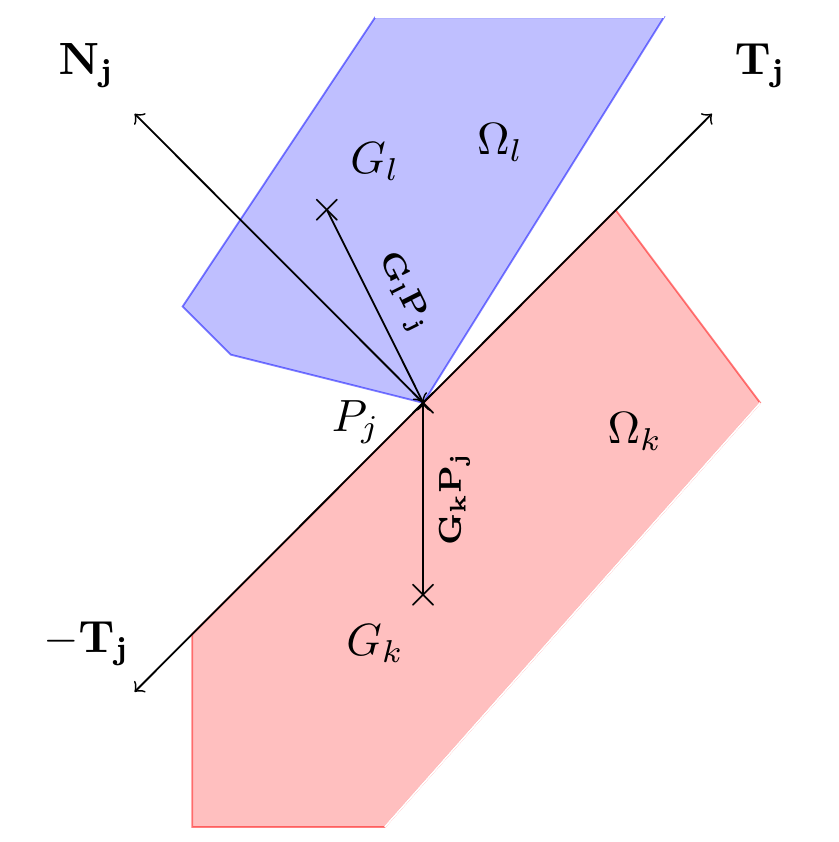
\includegraphics[width=.48\textwidth]{Collision1.png}
     \caption{Interaction entre deux floes $\Omega_k$ et $\Omega_l$ au point $P_j$ \parencite[p.26]{rabatel2015thesis}.}
     \label{fig:Collision1}
 \end{figure}

Soit $P_j$, ($j \in \{1,\ldots,n\}$) un point de contact entre les floes $\Omega_k$ et $\Omega_l$ (voir \cref{fig:Collision1}). Nous notons $\bvec{F}_{kj}(t)$ la force de contact du floe $\Omega_k$ au floe $\Omega_l$ appliquée en $P_j$. Par convention, une matrice de contact $\bmat{M_c}$ est définie telle que son coefficient $c_kj$ vaut :
 \begin{itemize}
     \item $0\,\,\,\,\,\, $ si le point de contact $P_j$ n’est pas un point de contact du floe $\Omega_k$ ;
     \item $-1$ si le point de contact $P_j$ est un point de contact entre les floes $\Omega_k$ et $\Omega_l$ avec $k < l$ ;
     \item $1\,\,\,\,\,\, $ si le point de contact $P_j$ est un point de contact entre les floes $\Omega_k$ et $\Omega_l$ avec $k > l$.
 \end{itemize}
En notant $E_k$ l’ensemble des points de contact du floe $\Omega_k$ au temps $t$, \citeauthor{rabatel2015thesis} définit la résultante des forces de contact $\bvec{F}^c_k(t)$ au floe $\Omega_k$ comme :
 $$
 \bvec{F}^c_k(t) = \sum_{j \in E_k} c_{jk} \bvec{F}_{kj}(t) \,.
 $$
En rajoutent ces forces aux forces extérieures lors du bilan des forces à l'\cref{eq:bilan1}, on obtient, pour un floe $\Omega_k(t)$ :
 \begin{align} \label{eq:bilan4}
     \mathcal{M} \frac{\diff W(t)}{\diff t} = \mathcal{H}(t) + \sum_{j \in E_k} \begin{pmatrix}
         \bvec{F}_{kj}(t) \\ \bvec{G}_k \bvec{P}_j \wedge \bvec{F}_{kj}(t) 
     \end{pmatrix} \,.
 \end{align}


\subsubsection{Formulation en problème linéaire de complémentarité}


Il existe deux principales manières de formuler le problème du contact entre deux solides rigides. L'auteur de \parencite{rabatel2015thesis} opte pour le formalisme vitesse-impulsion, au détriment du formalisme accélération-force. En effet, l’approche en \textbf{vitesse-impulsion} apporte l’avantage de pouvoir exprimer la force de friction de Coulomb directement par rapport à la vitesse. Il n’est pas nécessaire de connaître la nature du contact. Pour comprendre les travaux de \citeauthor{rabatel2015thesis}, il nous faut au préalable définir le notion d'impulsion. Sur un intervalle de temps $\delta t^*$, s’il y a un contact entre les floes $\Omega_k$ et $\Omega_l$ au point $P_j$, nous dirons que le floe $\Omega_k$ a subi un choc provenant du floe $\Omega_l$ au point de contact $P_j$ caractérisé par l’impulsion :
$$
\bvec{\mathcal{I}}_{kj} = \int_{\delta t^*} c_{kj} \bvec{F}_{kj}(t) \diff t \,.
$$ 
\citeauthor{rabatel2015thesis} fait donc apparaître les impulsions dans les équations des moments (\ref{eq:bilan1}) pour le floe $\Omega_k$ sur l’intervalle temporel $\delta t^*$ :
$$
\mathcal{M}_k \int_{\dtstar} \dot{W}_k(t) \diff t = \int_{\dtstar} \mathcal{H}(t) \diff t + \sum_{j \in E_k} \begin{pmatrix}
    \bvec{\mathcal{I}}_{kj} \\ \bvec{G}_k \bvec{P}_j \wedge \bvec{\mathcal{I}}_{kj} 
\end{pmatrix} \,.
$$
En écrivant $\dtstar = [t^{-}, t^{+}]$, on peut donc introduire les inconnues $\beta$, $\lambda \in (\Rdeux)^m$ \footnote{La variable $m$ désigne le nombre total de contraintes unilatérales dans le système.} pour le problème de contact :
\begin{align}
    \mathcal{M} \left( W(t^{+}) - W(t^{-}) \right) = \int_{\dtstar} \mathcal{H}(t) \diff t + \bmat{B}\beta + \bmat{J}\lambda \,,
\end{align}
où $\bmat{B}$ et $\bmat{J}$ sont deux matrices de $(\Rtrois)^{n \times m}$ telle que :
\begin{align*}
    \bmat{B} = (d_{kj})_{\substack{1 \leq k \leq n \\ 1 \leq j \leq m}} \,, \quad d_{kj} = \,
    \begin{cases}
        0 \in \Rtrois &\text{ si } P_j \text{ n'est pas un point de contact de } \Omega_k \,, \\
        \begin{pmatrix}
            c_{kj} \bvec{T}_{j} \\ c_{kj} \bvec{P}_j\bvec{G}_k \wedge \bvec{T}_j 
        \end{pmatrix} &\text{ si } P_j \text{ est un point de contact de } \Omega_k \,,
    \end{cases}  \\
    \bmat{J} = (s_{kj})_{\substack{1 \leq k \leq n \\ 1 \leq j \leq m}} \,, \quad s_{kj} = \,
    \begin{cases}
        0 \in \Rtrois &\text{ si } P_j \text{ n'est pas un point de contact de } \Omega_k \,, \\
        \begin{pmatrix}
            c_{kj} \bvec{N}_{j} \\ c_{kj} \bvec{P}_j\bvec{G}_k \wedge \bvec{N}_j 
        \end{pmatrix} &\text{ si } P_j \text{ est un point de contact de } \Omega_k.
    \end{cases}
\end{align*}
Les matrices $\bmat{B}$ et $\bmat{J}$ sont obtenues par décomposition des forces de contact dans le repère de contact $\mathcal{R}_{\Omega_j} = (P_j, \bvec{T}_j, \bvec{N}_j)$ (voir \cref{fig:Collision1}).

Comme précédemment mentionné, afin de modéliser la friction dans une collision qui respecte la loi de Coulomb, \parencite{rabatel2015thesis} se base sur les travaux de Stewart et Trinkle \parencite{stewart1996implicit} qui définissent une condition de complémentarité reliant la composante tangentielle $\beta_j$ de l'impulsion appliquée au point $P_j$, la composante normale $\lambda_j$, la vitesse relative tangentielle du point $P_j$ et le coefficient de friction $\mu$. On introduit le vecteur $\tilde{\beta}$ contenant les composantes de l'impulsion tangentielle dans chacune des directions possibles de glissement $\bvec{T}_j$ ou $-\bvec{T}_j$. Il devient alors possible de formuler le problème de contact (sur tout le système $S$) sans interpénétration par le problème linéaire de complémentarité de l'\cref{eq:bilan3}. Dans cette formulation, l’impulsion de contact est effectivement à l’intérieur du cône de Coulomb :
\begin{align} \label{eq:bilan3}
\begin{dcases} \,\,
    \begin{pmatrix}
        0 \\ \bvec{w} \\ \gamma \\ \sigma 
    \end{pmatrix} =  
    \begin{pmatrix}
        \mathcal{M} &  -\bmat{J} & -\bmat{D} & 0 \\
        \bmat{J}^T & 0 & 0 & 0 \\
        \bmat{D}^T & 0 & 0 & \bmat{H} \\
        0 & \mu & -\bmat{H}^T & 0
    \end{pmatrix} 
    \begin{pmatrix}
        W(t^+) \\ \lambda \\ \tilde{\beta} \\ \alpha
    \end{pmatrix} + 
    \begin{pmatrix}
        \int_{\delta t^*} \mathcal{H}(t) \diff t - \mathcal{M} W(t^{-}) \\ 0 \\ 0 \\ 0
    \end{pmatrix} \,, \\ \quad
    \begin{pmatrix}
        \bvec{w} \\ \gamma \\ \sigma
    \end{pmatrix} \geq 0 \,, \quad
    \begin{pmatrix}
        \lambda \\ \tilde{\beta} \\ \alpha
    \end{pmatrix} \geq 0 \,, \quad
    \begin{pmatrix}
        \bvec{w} \\ \gamma \\ \sigma
    \end{pmatrix} \cdot
    \begin{pmatrix}
        \lambda \\ \tilde{\beta} \\ \alpha
    \end{pmatrix}  
     = 0 \,,
\end{dcases}
\end{align}
avec :
\begin{align*}
    &\bvec{w} = \bmat{J}^T W(t^+) \,, \quad
    \bmat{H}^T = (e_{ij})_{\substack{1 \leq i \leq m \\ 1 \leq j \leq 2m}} \,, \quad \tilde{\beta} = (\tilde{\beta}_j)_{1\leq j \leq m} \,, \quad \lambda = (\lambda_j)_{1 \leq j \leq m} \,, \\
    &\mu \text{ est la matrice diagonale de diagonale } (\mu_1,\dots, \mu_m) \,,\\
    &e_{ij} = \begin{cases}
        1 \text{   si } j = 2(i-1) + 1 \text{ ou } j=2(i-1) + 2 \,, \\
        0 \text{   sinon} \,,
    \end{cases} \\
    &D = (\bvec{B}_1 \vert - \bvec{B}_1 \vert \ldots \vert \bvec{B}_m \vert -\bvec{B}_m) \, \text{   avec } \bvec{B}_j \text{ la colonne } j \text{ de la matrice } \bmat{B} \,.
\end{align*}
Le problème consiste alors à trouver les vitesses après contact $W(t^{+})$, à l’aide des composantes tangentielles et normales des impulsions dans les repères de contact $(\tilde{\beta},\,, \gamma)$, elles-mêmes inconnues du système.


\subsubsection{Consistance énergétique}


D'après l'auteur de \parencite[p.42]{rabatel2015thesis}, traiter le problème de contact à partir de lois non régulières ne permet pas d’obtenir des solutions satisfaisant à la fois la non-interpénétration, la friction de Coulomb et une consistance énergétique. En se focalisant sur la consistance énergétique, \citeauthor{rabatel2015thesis} a subdivisé le problème en deux : une phase de compression et une phase de décompression suivant la loi de Poisson. La \textbf{phase de compression} modélise la capacité maximale des floes à emmagasiner, par la déformation, une partie ou la totalité de l’énergie cinétique transmise lors du contact. L'impulsion normale $\lambda^c$ calculée durant cette phase (en résolvant le problème de complémentarité (\ref{eq:bilan3})) correspond à un coefficient de restitution $\varepsilon = 0$. Les impulsions obtenues durant cette phase sont celles nécessaires pour éviter l'interpénétration, et correspondent donc à une énergie cinétique maximale emmagasinée. La \textbf{phase de décompression} correspond à la restitution partielle ou complète de l’énergie cinétique emmagasinée par la déformation des floes. L’impulsion lors de cette phase, notée $\lambda^d$, est déterminée par $\lambda^d = \varepsilon \lambda^c$ (l’hypothèse de Poisson \parencite{glocker1995multiple}). Durant la phase de décompression, \citeauthor{rabatel2015thesis} a donc opté pour la consistance énergétique et la non-interpénétration avec la solution :
$$
W^N = (1 + \varepsilon)W^{c} - \varepsilon W(t^{-}) \,,
$$
où $W^c$ représente les vitesses des floes après la phase de compression, et $\varepsilon$ le coefficient de restitution pour les contacts considérés inélastiques.

% \subsubsection{Traitement des conditions aux bords}

\subsubsection{Le modèle de l'environnement}


L’environnement est l’ensemble des forces extérieures qui agissent sur les floes hormis les forces de contact décrites dans les sections précédentes. Ces principales forces sont:
\begin{itemize}
    \item La force de Coriolis $\bvec{\mathfrak{F}}_c$ donnée pour un floe $\Omega_i(t)$ par:
    $$
    \bvec{\mathfrak{F}}_{c,i}(t) = -f\bvec{k} \wedge \dot{\bvec G}_i(t) \,,
    $$
    avec $f$ le paramètre de Coriolis et $\bvec{k}$ le vecteur dirigé vers le haut dans le repère absolu $\mathcal{R}_{abs}$.
    \item Les forces de trainée associées au vent $\bvec{\tau}_a(t)$ et celle associée à l'océan $\bvec{\tau}_w(t)$: 
    \begin{align*}
        \bvec{\tau}_a(t) &= \rho_a C_a \Vert \bvec{U}_a(t) \Vert \bvec{U}_a(t) \,, \\        
        \bvec{\tau}_w(t,P) &= \rho_w C_w \Vert \bvec{U}_w(t) - \dot{P}(t) \Vert \left(\bvec{U}_w(t) - \dot{P}(t) \right) \,,
    \end{align*}
    avec $\rho$ la masse volumique du fluide (l'indice $a$ pour l'air et $w$ pour l'eau) et $C$ un coefficient de traînée sans dimension (voir [HI86]) ; $\bvec{U}_a$, $\bvec{U}_w$, $\dot{P}(t)$ respectivement la vitesse du vent à l'interface glace/fluide, la vitesse du courant oceanique à l'interface glace/fluide, et la vitesse d'un point $P$ du floe. 
\end{itemize}
Le modèle de dynamique régulière définit en \cref{eq:bilan1} peut se voire expliciter:
\begin{align*}
    \begin{dcases}
            M_i \frac{\diff \dot{\bvec{G}}_i(t)}{\diff{t}} &= M_i \mathfrak{F}_{c,i}(t) + \int_{\Omega_i(t)} \bvec{\tau}_a(t) + \bvec{\tau}_w(t,P) \diff s \,,\\
            \mathcal{I}_i \frac{\diff \dot{\theta}_i(t)}{\diff t} &= \int_{\Omega_i(t)} \bvec{G}_i\bvec{P} \wedge \left(\bvec{\tau}_a(t) + \bvec{\tau}_w(t,P)\right) \diff s \,.
    \end{dcases}
\end{align*} 
L'algorithme décrivant en détail le processus de collision ainsi que la consistance énergétique se trouve à la page 43 du document \parencite{rabatel2015thesis}.


\subsection{Méthodes numériques et algorithmiques pour la résolution du problème}
 
\subsubsection{Discrétisation temporelle}

Pour simuler la dynamique des floes de glace soumis a des forces extérieures et possiblement des collisions, il faut intégrer la dynamique régulière, et la dynamique non régulière ; et il existe deux principales méthodes pour la discrétisation en temps dans de tels problèmes. La méthode \textit{\textbf{time-stepping}} (voir \parencite{acary2013projected} pour les schémas de Moreau \parencite{moreau1986dynamique,jean1999non}, et de Schatzman-Paoli \parencite{paoli2002numerical,paoli2002numerical2} par exemple, pour lesquels une convergence a pu être exhibée à partir de la convergence en graphe de Moreau \parencite{moreau1978approximation}). Comparé aux autres méthodes, la méthode \textit{time-stepping} traite mieux les points d'accumulation \parencite[p.58]{rabatel2015thesis} ; et est plus performante sur des problèmes de multiples contacts. Cependant, \citeauthor{rabatel2015thesis} opte pour le schéma \textit{\textbf{event-driven}} pour sa précision dans la localisation des collisions et sa facilité de manipulation. En plus, elles permettent d’utiliser des schémas d’intégration existant d’ordre élevé pour des équations différentielles ordinaires. Le seuil de collision choisi est suffisamment grand pour éviter de traiter les collisions une par une. Le schéma utilisé pour intégrer l'\cref{eq:bilan1} est un schéma du type Euler explicite, pour sa facilité d’implémentation, pour sa facilité à prédire la localisation en espace et en temps des futures collisions, et enfin, pour sa capacité à dépasser les problèmes de points d’accumulation. 

La simulation par la méthode \textit{event-driven} demande la définition d'un pas de temps maximal pour lequel le schéma reste stable. Le pas de temps $\Delta t_{max}$ sera utilisé si aucune collision n'est détectée entre les instants $t$ et $t + \Delta t_{max}$. En se référant au modèle idéalisé 1D (voir \parencite[p.49]{rabatel2015thesis}), \citeauthor{rabatel2015thesis} distingue deux critères pour la stabilité du schéma numérique au temps $t$ :
\begin{itemize}
    \item lorsque la vitesse caractéristique des floes $V_c(t) = N_a \bvec{U}_a(t) + \bvec{U}_w(t)$ est constante sur l'intervalle de simulation $I$, alors pour :  
    \begin{align} \label{eq:dtmax1}
        \Delta t \leq \Delta t_{max} = \min{ \left(\frac{\rho}{2 \vert \bvec{U}_a(t) \vert \sqrt{\rho_a C_a \rho_w C_w}} \,, \,\frac{2K_t}{L_t} \right)}
    \end{align}
    avec :
    $$
    L_t = \rho^{-1} \rho_w C_w \left( N_a^2 \bvec{U}_a^2 + (N_a\bvec{U}_a + 2 \bvec{U}_w)^2 \right) \,, \text{ et  } K_t = \vert V_c(t) \vert \text{ constant, }
    $$
    le schéma est stable c-à-d $\dot{\bvec{G}} (t + \Delta t) \in [-K_t, K_t] = [-K_{t + \Delta t}, K_{t + \Delta t}]$ ;
    \item lorsque les variations de $V_c(t)$ entraînent une augmentation de $K_t$ au cours du temps. La propriété de stabilité reste vérifiée car :$$\dot{\bvec{G}} (t + \Delta t) \in [-K_t, K_t] \subset [-K_{t + \Delta t}, K_{t + \Delta t}] \,;$$
    \item lorsque les variations de $V_c(t)$ entraînent une diminution stricte de $K_t$ au cours du temps, alors la condition de stabilité dans les deux cas précédents ne peut être vérifiée. \citeauthor{rabatel2015thesis} introduit donc une seconde définition de la stabilité pour traiter ce cas. Il remarque que pour : 
    \begin{align} \label{eq:dtmax2}
    \Delta t_{max} \leq \begin{dcases}
        \frac{-2x}{\tilde{L}_t^{-}} \text{  si  } x \in  ]-\infty, K_{t+\Delta t}] \,, \\
        \frac{-2x}{-\tilde{L}_t^{+}} \text{  si  } x \in  ]K_{t+\Delta t}, +\infty] \,,
    \end{dcases}\end{align}
    avec : \begin{align*} \tilde{L}_t^{-} =  \rho^{-1} \rho_w C_w \left[ N_a^2 \bvec{U}_a(t+\Delta t)^2 - (\bvec{U}_w(t + \Delta t) - x)^2 \right] \,, \\ \tilde{L}_t^{+} =  \rho^{-1} \rho_w C_w \left[ N_a^2 \bvec{U}_a(t+\Delta t)^2 + (\bvec{U}_w(t + \Delta t) - x)^2 \right] \,,
     \end{align*}
    ce qui conduit à la diminution de la vitesse des floes.
\end{itemize} 
En conclusion, pour une vitesse infinitésimale initiale $\dot{G}(0) \in [-K_0, K_0]$, pour tout $t \in I$, et pour tout $\Delta t_{max}$ vérifiant les \cref{eq:dtmax1,eq:dtmax2}, nous avons les vitesses des floes majorées par :
$$
\max_{t \in I}{K_t}.
$$
\citeauthor{rabatel2015thesis} choisi donc de prendre :
$$
\Delta t_{max} = \min{  \left\{ \frac{3}{4} \left( \frac{ -2 \max_{t \in I}{K_t} }{ \max_{t \in I}{\tilde{L}_t^{-}}} \right),  \frac{3}{4} \left(\frac{2 \max_{t \in I}{K_t}  }{ \max_{t \in I}{-\tilde{L}_t^{+}}}\right), \frac{\rho}{2 \left(  \max_{t \in I}{  \vert \bvec{U}_a(t) \vert } \right)  \sqrt{\rho_a C_a \rho_w C_w}} \right\}} \,,
$$
pour s'assurer que le modèle idéalisé vérifie les critères de stabilité définis. 
Notons que le procédé global d’intégration de la dynamique pour le modèle se trouve dans \parencite[p.60]{rabatel2015thesis}; le schéma est repris à la \cref{fig:Algo1}.

\begin{figure}[!ht]
    \centering
    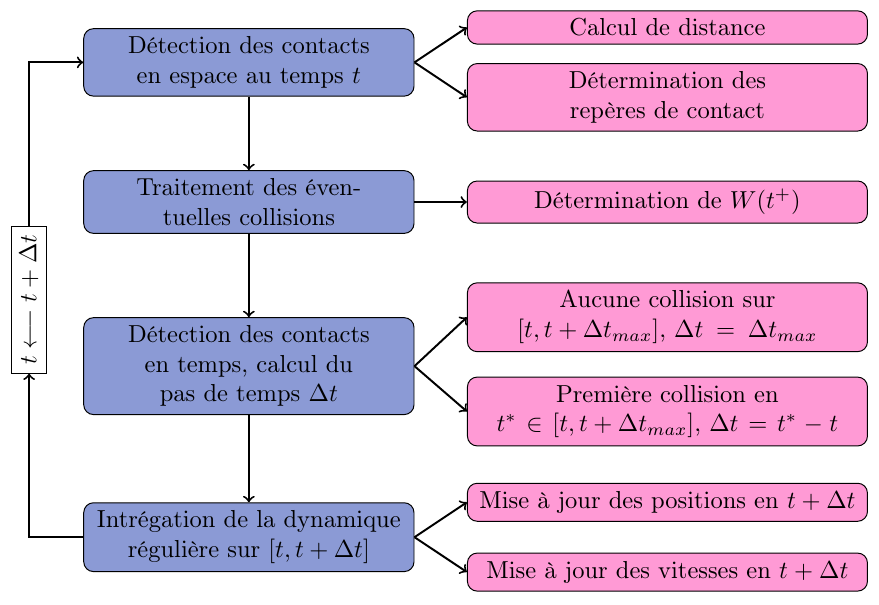
\includegraphics[width=.72\textwidth]{Algo1.png}
    \caption{Procédé global d’intégration de la dynamique pour notre modèle \parencite[p.60]{rabatel2015thesis}.}
    \label{fig:Algo1}
\end{figure}


\subsubsection{Détection des collisions en espace}

Des deux méthodes principales utilisées dans la littérature pour la détection des voisins, \citeauthor{rabatel2015thesis} a choisi la méthode de \textbf{hiérarchie de volumes englobants} pour sa facilité de mise en place et pour son efficacité même avec de grands ratios de tailles. L'alternative était la méthode de \textbf{partitionnement de l'espace} qui elle, souffre de plusieurs défauts non surmontables pour le modèle développé. Les méthodes de volumes englobants consistent à englober le contour de l’objet par des volumes à des échelles de plus en plus fines pour améliorer la détection.

\subsubsection{Détection des contacts en temps}

Il s'agit ici de trouver le pas de temps optimal : c’est-à-dire un pas de temps $\Delta t$ pour lequel la configuration des floes ne contient pas d’interpénétrations sur l’intervalle de temps $[t, t + \Delta t]$ et, pour tout $\varepsilon > 0$, contient au moins une interpénétration sur l’intervalle de temps $[t + \Delta t, t + \Delta t + \varepsilon]$ \parencite[p.87]{rabatel2015thesis}.
Lorsque le critère de collision n’est pas vérifié, \citeauthor{rabatel2015thesis} montre qu'il suffit de prendre :
$$
\Delta t_{i,j} = -\frac{\delta_{i,j}(t) - tol_3}{\bvec{A}_{ij}(t) \cdot \left( \dot{G}_i(t) - \dot{G}_j(t) \right)} \,,
$$
avec :
$$
\bvec{A}_{i,j}(t) = \frac{C_{0,i}(t) - C_{0,i}(t)}{d\left(C_{0,i}(t), C_{0,i}(t) \right)} \,, \text{ et  } \quad tol_3 = \frac{\xi}{20} \,,
$$
où $C_{0,i}(t)$ désigne le centre du volume englobant de niveau $0$ du floe $\Omega_i(t)$. Lorsque le critère de collision est vérifié, il faut plutôt prendre :
$$
\Delta t_{i,j} = \frac{\min{\left( \eta_i, \eta_j \right) - tol_3}}{\Gamma(t)} \,,
$$
avec :
$$
\Gamma(t) = \max{\left( \Vert \dot{Q}_i^{i,j}(t) \Vert \,, \, \Vert \dot{Q}_j^{j,i}(t) \Vert  \right)} \,,
$$
où $\dot{Q}_i^{i,j}$ représente la distance parcourue par un point de $\Omega_i (t)$ relativement à $\Omega_j (t)$. Une fois ce $\Delta t_{i,j}$ assurant la non-interpénétration trouvé, on peut donc choisir 
$$
\Delta t = \min{\left( \Delta t_{max} \,, \min_{ \substack{ (i,j) \in \left\{ 1,\ldots,n \right\}^2 \\ i \neq j}}{\Delta t_{i,j}} \right)} \,.
$$
Le lecteur est renvoyé au document \parencite[p.91]{rabatel2015thesis} pour plus de détails sur la détection des contacts en temps.

\subsubsection{Construction des repères de contacts}

La construction d'un repère de contact n'est effectuée que lorsque le contact entre deux floes $\Omega_k$ et $\Omega_l$ est \textbf{linéique} \parencite[p.79]{rabatel2015thesis}, ou \textbf{ponctuel} et le vecteur porté par les points en contacts appartient au cône normal de $P$. La normale $\bvec{N}$ est alors déterminée comme le vecteur unité dirigé par $\bvec{PQ}$. Si $Q$ n’est pas unique, on se retrouve dans la situation où il peut exister plusieurs repères de contact pour un point de contact. Dans les autres cas, le repère de contact associé au point $P$ n’est pas construit et $P$ n’est pas considéré dans le traitement des contacts \parencite[p.80]{rabatel2015thesis}. L'algorithme de détection des points de contacts afin de construire les repère de contact est explicité dans le document \parencite[p.76]{rabatel2015thesis}. 


\subsubsection{Simulation des événements collisions}

Une fois les voisins détectés et les repères de contact construits, on peut passer à la prochaine étape qui consiste en la simulation des évènements de collisions. Ici, plusieurs choix s'offrent à nous : les méthodes dites de \textbf{régularisations}, les méthodes dites \textbf{itératives}, et les méthodes dites \textbf{de pivots} \parencite[p.82]{rabatel2015thesis}. La première catégorie est adaptée aux modèles régularisants, ce qui n'est le cas de notre modèle. La deuxième par contre a extensivement été utilisée dans la littérature ; on peut citer Moreau \parencite{moreau1988unilateral,moreau1999numerical,jean1999non}, Aitken \parencite{aitken1950iv}. Malheureusement, dès que la matrice $A$ du problème de complémentarité à résoudre n'est plus symétrique, ce deuxième groupe de techniques ne s'avère pas efficace. \citeauthor{rabatel2015thesis} choisi donc l'algorithme de Lemke pour lequel il existe des preuves de convergence lorsque la matrice $A$ est copositive. Bien qu'il soit performant, il faut néanmoins noter que l’algorithme de Lemke étant une technique globale c’est-à-dire traitant les contacts simultanément, ne garantit pas une bonne propagation du contact \parencite[p.82]{rabatel2015thesis}.

\subsubsection{Optimisations}

La première optimisation apportée est celle sur les distances de collision : deux floes sont en contact si la distance entre eux n'est pas nulle, mais supérieure à un seuil appelée \textbf{distance de collision}.

La deuxième concerne la condition de non-interpénétration \parencite[p.85]{rabatel2015thesis}. En cas de congestion, il est difficile que les floes décollent après contact. En exigeant que $\bmat{J}^T W(t^+) > 0$ après collision, on risque ne pas avoir de solution pour le problème linéaire de complémentarité associé. \citeauthor{rabatel2015thesis} relaxe donc la condition de Signorini en définissant un réel $c$, et l'ensemble des vitesses admissibles devient donc :
$$
V_c = \left\{ w \in \mathbb{R}^{3n} \, | \, \bmat{J}^T w \geq c \right\} \,.
$$

Une troisième optimisation concernant la définition de la \textbf{notion d'erreur} et de \textbf{tolérance} a été implémentée. La quatrième consiste en la résolution d'un LCP en trois tentatives (avec trois algorithmes de Lemke différents) même si cela augmente les coups de calculs \parencite[p.86]{rabatel2015thesis}. 

Si la troisième optimisation ne s'avère pas suffisance, une dernière optimisation consiste en la modification aléatoire de certains coefficients de la matrice $A$, la permutation des lignes afin d'éviter des zéros sur la diagonale, ou encore l'utilisation de la notion de \textbf{contact actif}.


\subsection{Validations et exploitations du modèle}

Les résultats ont été validés à travers plusieurs expériences. Nous citons des exemples classiques tels que la \textbf{boîte glissante}, le \textbf{berceau de Newton}, le \textbf{canon de Newton}, la \textbf{balle rebondissante}, etc. Le modèle a ensuite été validé sur des scénarios simples de dérive libre soumise à des courants océanique et atmosphérique, et des scénarios simples de collision. En effet, il a été vérifié que le comportement d’un objet simulé est cohérent avec le comportement théorique et avec les observations. Les principes physiques suivants ont ainsi pu être testé par \citeauthor{rabatel2015thesis} :
\begin{itemize}
    \item la conservation de la symétrie d’une configuration ;
    \item la satisfaction du modèle de Coulomb ;
    \item le traitement d’un point d’accumulation ;
    \item la cohérence temporelle ou la propagation des ondes de choc ;
    \item la conservation de l’énergie cinétique.
\end{itemize} 
Des telles exploitations telles que la dérive dans un canal étroit, pour des floes en bassins a été étudié (voir \cref{fig:Derive,fig:DeriveSol}). Aussi, la dérive soumise à un vent et un courant variable avec des vitesses du vent provenant de \textbf{ERAinterim}, à partir du modèle glace de mer et océan \textbf{TOPAZ} a été étudiée.

\begin{figure}[!ht]
    \centering
    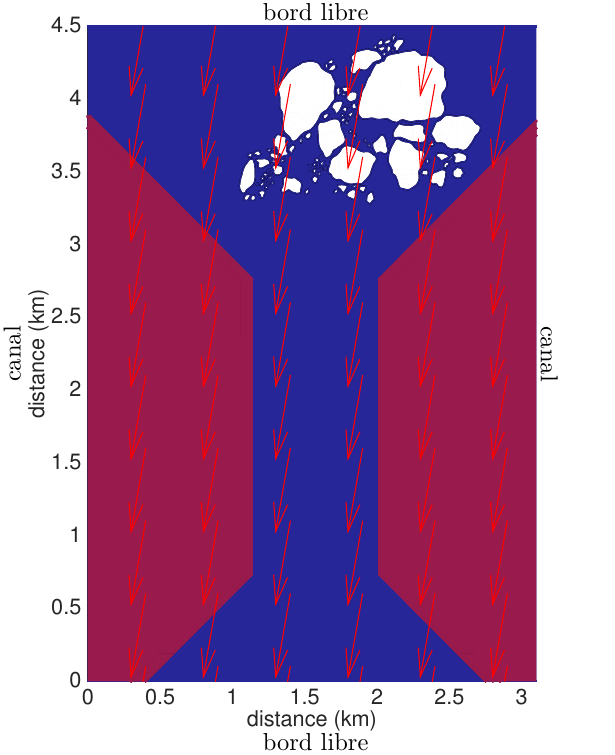
\includegraphics[width=.38\textwidth]{Derive.png}
    \caption{Configuration à l’instant initial pour le scénario de dérive dans un canal étroit \parencite[p.124]{rabatel2015thesis}.}
    \label{fig:Derive}
\end{figure}

\begin{figure}[!ht]
    \centering
    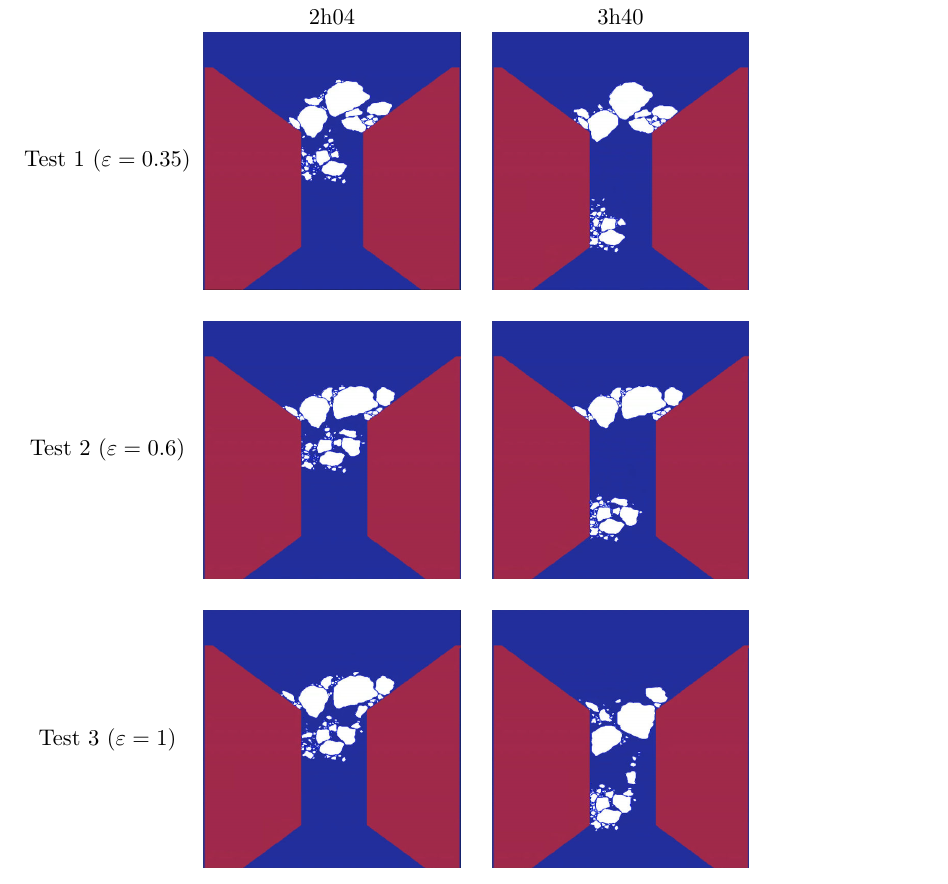
\includegraphics[width=.78\textwidth]{DeriveSol.png}
    \caption{Quelques résultats obtenus à deux heures différentes de la configuration des floes pour différentes valeurs du coefficient de restitution $\varepsilon$ \parencite[p.126]{rabatel2015thesis}.}
    \label{fig:DeriveSol}
\end{figure}

\subsection{Discussion}
Bien que les travaux de \citeauthor{rabatel2015thesis} ont été testés et validés sur plusieurs configurations différentes, il reste néanmoins des points qui ne sont pas traités, et qui ont très clairement été soulignés dans la thèse \parencite{rabatel2015thesis} :
\begin{enumerate}
    \item Le modèle ne gère pas la rhéologie\footnote{La rhéologie est l'étude de la déformation et de l'écoulement de la matière sous l'effet d'une contrainte appliquée.} de la glace : les floes sont des solides purement rigides (ils ne se déforment pas) et la dissipation d’énergie cinétique durant la collision est décrite en utilisant un coefficient purement empirique de restitution $\varepsilon$.  
    \item La loi de contact utilisée pour le glissement (voir \parencite{stewart1996implicit}), bien que très riche, ne prends pas en compte toutes les vitesses possibles de déplacement. La construction d’une loi qui donnerait accès à la région entière demanderait de prendre en compte un grand nombre de phénomènes intrinsèques aux contacts. Leur compréhension et leur rôle à chacun est difficile à déterminer. 
    \item Les coefficients de friction et de restitution utilisées sont limitants. En réalité, il n’est pas possible de prendre en compte ou d'interpréter mathématiquement certains effets lors du contact ; c'est le cas par exemple avec la dispersion de l'énergie (voir \parencite{nguyen2014multiple}). Cette dispersion est la conséquence de certains effets vibratoires à travers une chaîne de contact. Seuls les effets de dissipation dus aux phénomènes locaux comme l’endommagement, la viscosité ou la plasticité sont pris en compte à travers l’utilisation des coefficients de restitution et de friction.
    \item Les vitesses obtenues après la phase de décompression afin d'assurer la dissipation de l'énergie cinétique possèdent une faiblesse : elles ne sont solutions que sous certaines conditions, comme le fait que les chocs soient frontaux et qu’il n’y ait pas d’apport des forces extérieures autres que les forces de contact durant la collision \parencite[p.41]{rabatel2015thesis}.
\end{enumerate}

















%%3----------------------------------------------------------------------------------------


\section{Résumé de thèse de D. Balasoiu}








Les travaux de D. Balasoiu concernent la modélisation et la simulation du comportement mécanique de floes de glace \parencite{balasoiu2020halthesis}. Il s'agit d'une amélioration du modèle de M. Rabatel, S. Labbé, et J. Weiss \parencite{rabatel2015thesis,rabatel2015dynamics} prenant en compte la fracture des floes. Précisément, ce travail se focalise sur l’initiation de la fracture, ainsi que la prédiction du chemin que la fracture emprunte. Jusqu’à présent, les floes étaient considérés comme des corps rigides; mais dans sa thèse, \citeauthor{balasoiu2020halthesis} les considère comme des corps élastiques. Son travail est divisé en deux parties. Il commence par proposer un modèle efficace pour la fracture fragile d’un floe de glace, lorsque celui-ci est soumis à un déplacement quasi-statique de son bord (une condition au bord de type Dirichlet). Puis, dans un second temps, il cherche à obtenir l’expression du déplacement au bord d’un floe qui est percuté par une masse ponctuelle.

\subsection{Théorie de la fracture : état de l’art} 
 
La théorie de fracture la plus répandue de nos jours est due à A.A. Griffith. Dans ses travaux \parencite{griffith1921vi}, in invalide les résultats de C. Inglis \parencite{inglis1913stresses} qui ne tenaient pas en compte la taille de la fracture ; il présente donc la croissance d'une faille comme une compétition d'énergie entre l'énergie élastique\footnote{Aussi appelée énergie de déformation, elle diminue avec l'accroissement de la fracture.} et l'énergie de surface\footnote{Énergie nécessaire à la création des deux nouvelles surfaces (les bords de la fissure). Cette énergie augmente avec l'accroissement de la fracture.}. 
Le critère de Griffith est un critère thermodynamique qui stipule que la fracture progresse si et seulement si cela permet au matériau d’atteindre un état de moindre énergie. En effet, sur un matériau élastique $\Omega$ dont la frontière est subdivisée en deux zones $\partial \Omega_D$, et $\partial \Omega_N$, on pose \parencite[p.33]{balasoiu2020halthesis} :
\begin{align*}
    E_{el} &= \int_{\Omega} W (x, e(u)) \diff x  \,,   \\
    \mathcal{F}(t,\sigma(t)) &= \int_{\Omega} f_v (x)\cdot \varphi \diff x + \int_{\partial\Omega_N} f_s (x) \cdot \varphi \diff x \,, \\
    \mathcal{P}(t,\sigma(t)) &= \int_{\Omega \backslash \sigma(t) } W (x, \nabla\varphi (t, \sigma(t))) \diff x - \mathcal{F}(t,\sigma(t)) \,, 
\end{align*}
où :
\begin{itemize}
    \item $E_{el}$ est l'énergie élastique du matériau sans faille.
    \item $\sigma(t)$ représente la fracture au temps $t$, supposée à l'équilibre.
    \item $\mathcal{P}$ l’énergie potentielle du matériau qui possède une fracture de taille $\sigma(t)$ au temps $t$.
    \item $e(u)$ est le tenseur de Green-St Venant, qui représente la déformation locale du matériau.
    \item $\varphi = \identity + u$ représente le déplacement du matériau supposé suffisamment régulier.
    \item $W$ est la densité d’énergie du matériau élastique, supposé hyper-élastique.
    \item $f_s$ est la contrainte surfacique appliquée sur le bord $\partial \Omega_N$.
    \item $f_v$ est le champ de force volumique appliquée sur $\Omega$.
\end{itemize}
D'après le critère de Griffith \parencite[p.34]{balasoiu2020halthesis}, la fonction $\sigma(t)$ doit vérifier :
\begin{enumerate}
    \item $\dfrac{\diff \sigma(t)}{\diff t} \geq 0$ ;
    \item $-\dfrac{\diff \mathcal{P}}{\diff \sigma} (t,\sigma(t)) \leq k$ ;
    \item $\dfrac{\diff \sigma(t)}{\diff t} > 0 \Rightarrow -\dfrac{\diff \mathcal{P}}{\diff \sigma} (t,\sigma(t)) = k$.
\end{enumerate}

%\begin{figure}[!ht]
%    \centering
%    \frame{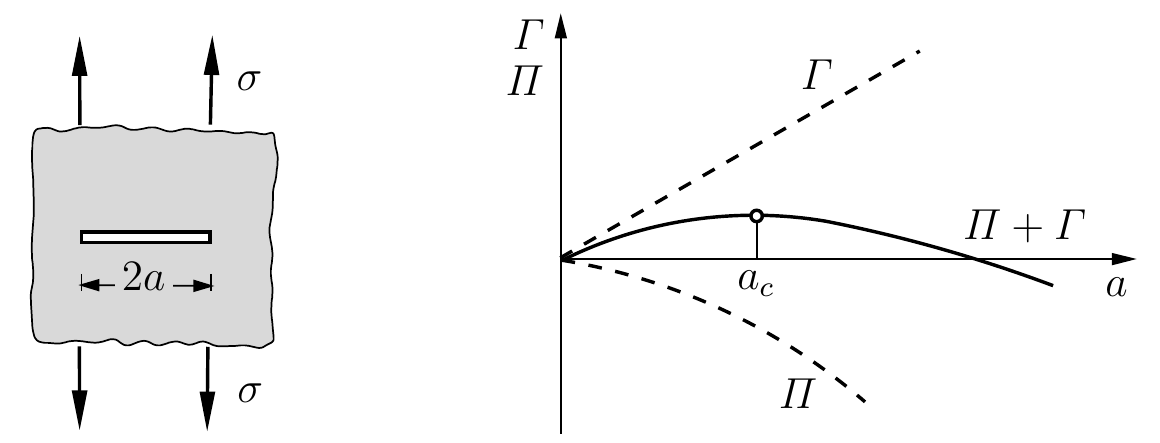
\includegraphics[width=.8\textwidth]{Griffith.png}}
%    \caption{Illustration du critère de Griffith \parencite{gross2017fracture}. ($\Pi$ et $\Gamma$ représentent les énergies potentielles et de fracture respectivement. \textit{Cette figure est à refaire manuellement !})}
%    \label{fig:Griffith}
%\end{figure}
%
%\noindent Une illustration de ce critère peut être observée à la \cref{fig:Griffith}. 

\noindent Comme mentionné plus haut, ce modèle souffre de problèmes de nucléation et de prédiction de la fracture. Pour contourner le problème de nucléation, les mécaniciens considèrent que tout matériau possède des microfissures, et ce sont ces dernières qui sont à l'origine des fissures observables à l'\oe{}il. Quant au problème du chemin emprunté par la fracture, A. Chambolle, G. Francfort et J.-J. Marigo \parencite{chambolle2009and} montrent que les critères d'Irwin \parencite{irwin1997analysis} sont invalides car, ils impliquent que, dans un matériau homogène et isotrope, le chemin de la fracture ne puisse être courbé.

Le modèle proposé par Francfort et Marigo \parencite{francfort1998revisiting} suit un résultat théorique dû à De Giorgi, M. Carriero et A. Leaci \parencite{de1989existence}, qui prouvent le théorème d’existence d'un minimum pour la fonctionnelle de Mumford-Shah qui intervient dans la détection des contours d’une image. Présentons donc les données géométriques du problème \parencite[p.37]{balasoiu2020halthesis}. Soit $\Omega \subset \mathbb{R}^N$ un ouvert connexe, dont la frontière $\partial \Omega$ est suffisamment lisse. On partitionne sa frontière :
$$
\partial \Omega = \partial \Omega_D \cup  \partial \Omega_N \,,
$$
où $\partial \Omega_D$ et $\partial \Omega_N$ sont les bords où l’on applique respectivement des conditions de Dirichlet et de Neumann. Sur la partie Dirichlet, on applique un déplacement du bord noté $U_D$, tandis que l’on laisse libre la partie de Neumann. On suppose également que le matériau est soumis à un champ de force volumique $f_v$. On suppose que $\Omega$ est un matériau hyper-élastique, dont la densité d’énergie est notée $W$. Ainsi, lorsque le matériau $\Omega$ subit (sans fracture) une déformation $\varphi = u + \identity$ suffisamment lisse, son énergie élastique vaut :
$$
\eel(u) = \int_{\Omega} W(x,e(u)) \diff x \,,
$$
où l’on a noté $u$ le champ de déplacement du matériau, et $e(u)$ son gradient symétrisé. On notera l’énergie élastique du matériau qui présente une fracture $\sigma$ :
$$
\eel(u,\sigma) = \inf_{u\in V_{U_D, \sigma}}{\int_{\Omega \backslash \sigma} W(x,e(u)) \diff x} \,,
$$
où l’on a défini l’espace fonctionnel :
$$
V_{U_D,\sigma} = \left\{ u \in H^1(\Omega \backslash \sigma, \mathbb{R}^N) \, \rvert \, u = U_D \text{ sur } \partial \Omega_D \right\} \,.
$$
Francfort et Marigo proposent ensuite l’énergie de fracture suivante sur :
$$
\efrac(\sigma) = \int_{\sigma} k(x) \diff \mathcal{H}^{N-1} \,,
$$
où le champ scalaire $k(x)$ traduit la ténacité du matériau, et est supposée strictement positive sur tout le matériau ; $\mathcal{H}^{N-1}$ représente la mesure de Haussdorf de dimension $N-1$, qui peut être comprise comme la longueur du contour pour $N=2$.
Ainsi, l’énergie totale du matériau vaut :
\begin{align*}
\etot(u,\sigma) &= \eel(u,\sigma) + \efrac(\sigma) \\
&= \int_{\Omega \backslash \sigma} W(x,e(u)) \diff x + \int_{\sigma} k(x) \diff \mathcal{H}^{N-1} \,,
\end{align*}
où $\sigma$ est une union dénombrable d'ensembles rectifiables. Ainsi donc, une solution du problème de fracture est un minimum de la fonctionnelle $\etot$. Signalons que \citeauthor{balasoiu2020halthesis} montre, dans le cas d'un mouvement antiplan\footnote{Un mouvement \textbf{antiplan} est un mouvement pour lequel le champ de déplacement $u$ est porté par un vecteur constant.}, que le modèle est quasiment identique au modèle de De Giorgi, M. Carriero et A. Leaci, pour lequel un théorème d'existence a pu être exhibé.

La méthode numérique employée est une approche à champ de phases. Elle repose sur la notion de $\Gamma$-convergence, en particulier sur le résultat de \textbf{convergence des minimums}. On remplace l'inconnue $\sigma$ par une suite de fonctions lisses $v_\varepsilon$. Par exemple, dans le cas du traitement d'image, pour la fonctionnelle de Mumford-Shah dont se sont inspiré Bourdin, Francfort et Marigo, on constate d'après Ambrosio et Tortorelli \parencite{ambrosio1990approximation} que la suite de fonctionnelle :
$$
G_{\varepsilon}(u,v) = \int_{\Omega} \left( \vert u-g \vert^2 + (v^2 + \eta_{\varepsilon}) \vert \nabla u \vert^2 + \varepsilon \vert \nabla v \vert^2 + \frac{(v-1)^2}{4\varepsilon} \right) \diff x \,,
$$
$\Gamma$-converge vers la fonctionnelle limite :
$$
G_f(u) = \int_{\Omega} \vert u-g \vert^2 + \vert \nabla u \vert^2 \diff x + \mathcal{H}^{N-1}(S_u) \,,
$$
où $\eta_{\varepsilon} = o(\varepsilon)$, $g:\Omega \mapsto [0,1]$ est la fonction de contraste de l’image, et $\mathcal{H}^{N-1}(S_u)$ est la restriction de la mesure de Hausdorff à l’ensemble des sauts de $u$, noté $S_u$, qui est un ensemble mesurable et composé d’une union dénombrable d’ensembles rectifiables \parencite[pp.35-37]{balasoiu2020halthesis}. Plusieurs études numériques reposant sur ce résultat de $\Gamma$-convergence sont disponibles dans la littérature. On cite par exemple ici les résultats obtenus dans \parencite{nagaraja2019phase} à la \cref{fig:PhaseField}.

\begin{figure}[!ht]
    \centering
    \begin{subfigure}[b]{0.9\textwidth}
        \centering
        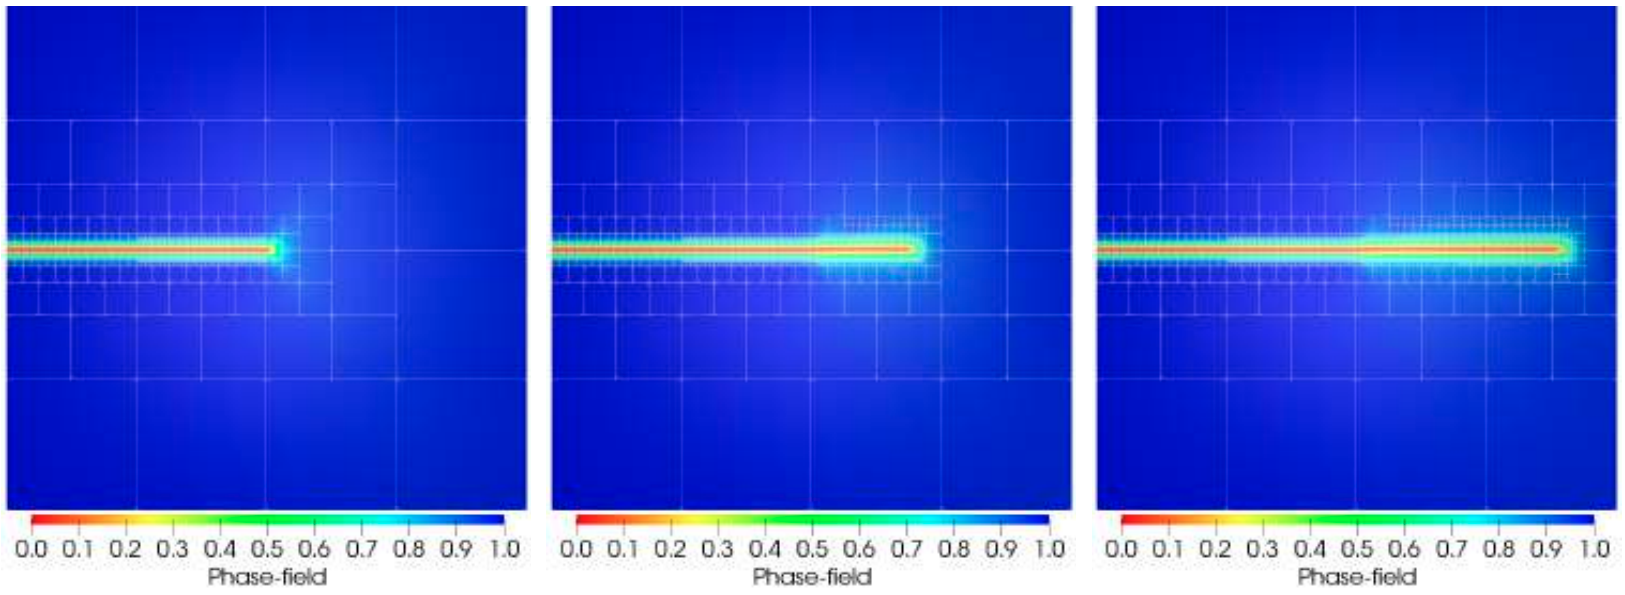
\includegraphics[width=\textwidth]{PhaseField1.png} 
        \caption{Croissance d’une fracture}
        \label{fig:PhaseField1}
    \end{subfigure}
    \begin{subfigure}[b]{0.9\textwidth}
        \centering
        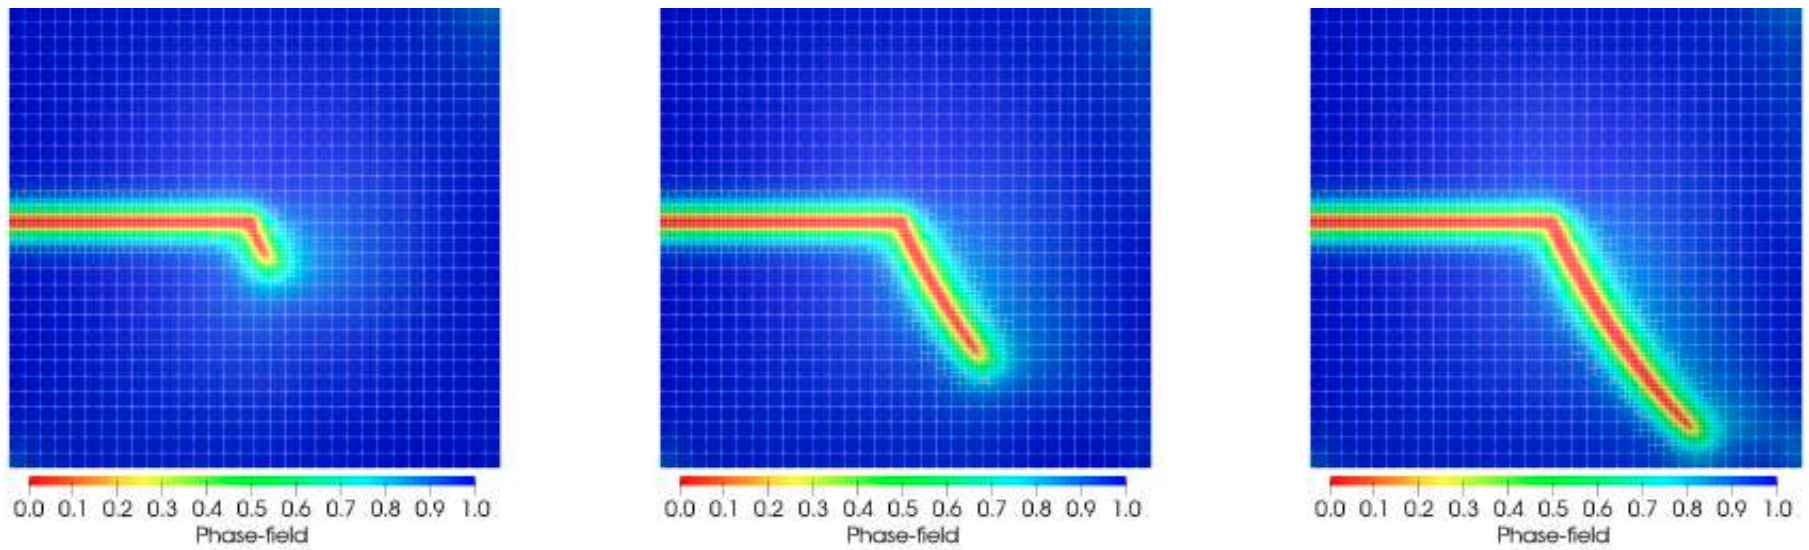
\includegraphics[width=\textwidth]{PhaseField2.png} 
        \caption{Bifurcation d’une fracture}
        \label{fig:PhaseField2}
    \end{subfigure}
    \begin{subfigure}[b]{0.9\textwidth}
        \centering
        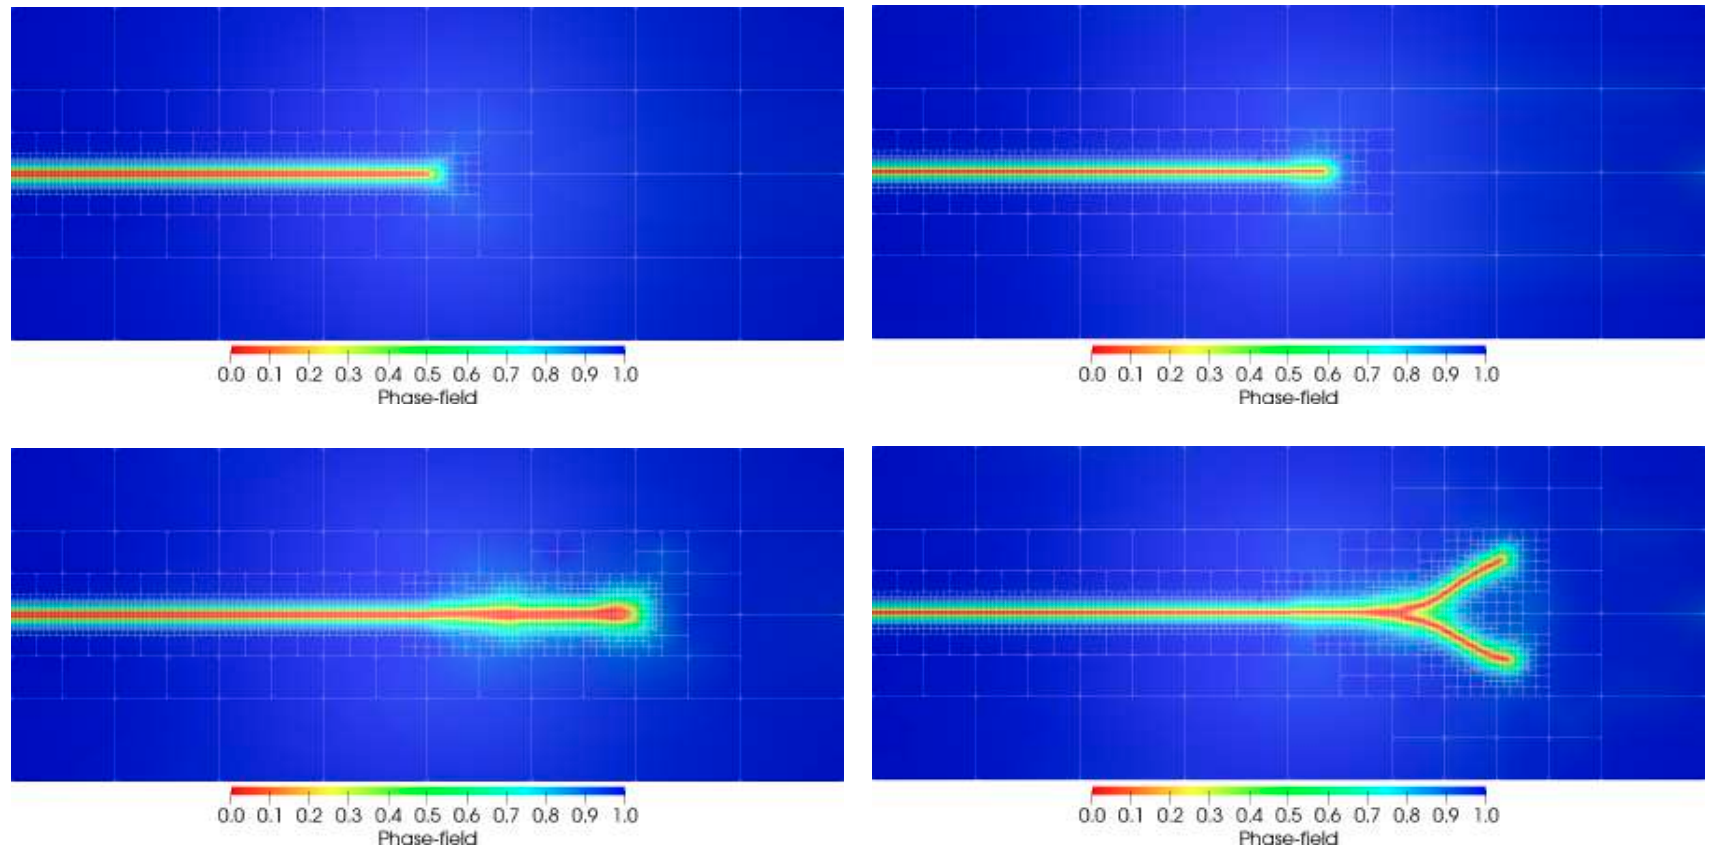
\includegraphics[width=\textwidth]{PhaseField3.png} 
        \caption{Branchement d’une fracture}
        \label{fig:PhaseField3}
    \end{subfigure}
       \caption{Trois résultats numériques obtenus dans \parencite{nagaraja2019phase} à l'aide d'une discrétisation éléments finis ($hp$-FEM) et volumes finis en ne remaillant le domaine que lorsque c'est nécessaire.}
       \label{fig:PhaseField}
\end{figure}


\subsection{Un modèle de fracture variationnel et efficace} 

Le modèle présenté dans la section précédente n'est pas adapté à notre étude. \citeauthor{balasoiu2020halthesis} a donc développé un modèle qui ne nécessite pas de fonctionnelle lissée, comme l'on fait plusieurs modèles de glaciologie (voir \parencite{lu2015plane}), en supposant que les fractures sont des segments. Un résultat d'existence (dans les cas où le floe n'est pas encore fracturé) est prouvé à l'aide de la convergence de Mosco. De plus, \citeauthor{balasoiu2020halthesis} introduit un problème d’évolution quasi-statique en appliquant progressivement la condition de Dirichlet sur une partie du bord du floe. Les fractures obtenues par ce problème d’évolution sont ainsi des lignes brisées. Le résultat d'existence n'a pas été prouvé pour ce dernier cas. Concernant le côté numérique, une méthode \textit{meshless}\footnote{Car l’ensemble discrétisé des fractures admissibles ne dépend pas du maillage utilisé.} est proposée.

Les modifications apportées pour traiter le modèle statique (dans $\Rdeux$) sont décrites ci-bas. Lorsqu'on fixe la fracture $\sigma$, l'énergie élastique prend la forme :
\begin{align*}
\eel (\cdot,\sigma): \, A_{\sigma} &\rightarrow \mathbb{R} \\
u &\mapsto \int_{\Omega \backslash \sigma} Ae(u) : e(u) \diff x \,,
\end{align*}
où $A$ représente le tenseur de Lamé du matériau, i.e.
$$
    \forall e \in M_2(\mathbb{R}), \quad Ae = \lambda \text{ tr}(e)I_2 + 2\mu e \,,
$$ 
où $\lambda$ et $\mu$ sont les coefficients de Lamé du matériau ; et l'ensemble des déplacements admissibles $A_{\sigma}$ est :
$$
A_{\sigma} = \left\{  u \in H^1 (\Omega \backslash \sigma, \mathbb{R}^2) \, \rvert \, u=U_D \text{ sur } \partial \Omega_D \backslash \sigma \text{ et } (u^+ - u^{-}) \cdot \nu \geq 0 \text{ sur } \sigma \right\} \,,
$$
avec $u^{+}$ et $u^{−}$ les restrictions de $u$ aux régions $\Omega^{+}$ et $\Omega^{-}$ respectivement (obtenues par extension de la fracture $\sigma$ de façon à ce qu'elle soit traversante \parencite[p.52]{balasoiu2020halthesis}), dans les directions $\nu$ (normale à la fracture orientée du bord vers le centre de $\Omega$) et $−\nu$. On note la présence d'une condition de type Signorini :
$$
(u^+ - u^{-}) \cdot \nu \geq 0 \text{  sur  } \sigma.
$$
L'énergie totale s'écrit :
\begin{align*}
\etot : \,\bigcup_{\sigma \in \Sigma } A_{\sigma} \times \left\{ \sigma \right\} &\rightarrow \mathbb{R} \\
 u &\mapsto \int_{\Omega \backslash \sigma} Ae(u) : e(u) \diff x + k\mathcal{H}^1(\sigma)\,,
\end{align*}
où $\Sigma$ représentent l'ensemble des segments orientés partant de la frontière donnée par :
$$
\Sigma = \left\{ [a,b] \in \mathbb{R}^2 \, \lvert \, a \in \partial\Omega, b\in \overline{\Omega}, ]a,b[ \in \Omega\right\} \,.
$$
Une solution de notre modèle de fracture fragile est un couple $(u^*, \sigma^*)$ qui vérifie:
$$
\etot(u^*,\sigma^*) = \min_{\sigma \in \Sigma}{\min_{u\in A_{\sigma}}{\etot(u,\sigma)}} \,.
$$
Ensuite, \citeauthor{balasoiu2020halthesis} remarque que la solution n'est pas unique. Il définit donc un problème d'évolution quasi-statique à la manière de \parencite{francfort1998revisiting}, en considérant un problème de chargement monotone : 
$$
U_D(t) = t\, U_D .
$$
On note $\overline{\Sigma}$ l’ensemble des lignes brisées de $\Omega$, sans point d’auto-intersection et qui partent de la frontière. On note également $\text{end}(\sigma)$ la fin d’une ligne brisée $\sigma \in  \overline{\Sigma}$.
On définit maintenant \parencite[p.50]{balasoiu2020halthesis}, pour toute ligne brisée $\sigma \in  \overline{\Sigma}$ l’ensemble des fractures admissibles partant de $\sigma$ :
$$
\Sigma_{\emptyset} = \Sigma \,, \quad \Sigma_{\sigma} = \left\{ \sigma \cup [a,b] \in \mathbb{R}^2 \, \lvert \, a = \text{end}(\sigma), b\in \overline{\Omega}, ]a,b[ \in \Omega\backslash \sigma \right\} \,.
$$
On définit également l'ensemble des déplacements admissibles associées :
$$
A_{t,\sigma} = \left\{  u \in H^1(\Omega \backslash \sigma , \mathbb{R}^2) \, \rvert \, u=tU_D \text{ sur } \partial \Omega_D \backslash \sigma \text{ et } (u^+ - u^{-}) \cdot \nu \geq 0 \text{ sur } \sigma \right\} \,,
$$
pour tout $t \in [0,1]$ et pour toute ligne brisée $\sigma$. De ces définitions, on peut exhiber un problème d'évolution discret, et un problème d'évolution continue en faisant tendre $t$ vers $0$. Le problème d’évolution continue admet des solutions, comme limite de solutions des problèmes d’évolutions discrets \parencite{dal2002model, chambolle2003density}.

Lorsque la fracture est fixée, \citeauthor{balasoiu2020halthesis} prouve l’existence de solutions à notre problème de minimisation, en utilisant la théorie des inégalités variationnelles, l'inégalité de Korn \parencite{ciarlet1988three} et le théorème de Lions-Stampacchia \parencite{lions1967variational}. Pour le cas statique, il montre que le problème a des solutions lorsque l’ouvert n’est pas encore fracturé, ceci en se servant principalement de la convergence de Mosco. Pour le modèle quasi-statique, un résultat d'existence n'a pas été trouvé, et une conjecture pour une ligne brisée qui possède un point d'auto-intersection a été proposée.



\subsection{Étude asymptotique d’un réseau de ressorts régulier} 

Dans ce chapitre, \citeauthor{balasoiu2020halthesis} souhaite approcher l’énergie élastique d’un matériau continu par l’énergie élastique d’un réseau de ressorts, dans un cadre statique, lorsque celui-ci est soumis à un déplacement de son bord. Autrement dit, nous ne nous intéressons pas au mouvement des particules, nous n’étudions que l’état d’équilibre du réseau de ressorts.

Commencions par quelques définitions pour le maillage sur un floe. Pour définir un réseau de ressort $\tau$, on définit l'ensemble de ses points $\tau_0$ disposés en forme de grille: 
$$
\tau_0 = \Omega \cap \mathbb{Z}^2.
$$
De façon similaire, l'ensemble des arêtes se nomme $\tau_1$, et l'ensemble des cellules $\tau_2$. Le réseau $\tau$ est obtenu à partir de $\tau_0$ en traçant les côtés de chaque carré ; à la frontière, on trace les diagonales des carrés incomplets. On note $W (\tau, \Rdeux)$ l’ensemble des fonctions de $\tau_0$ dans $\Rdeux$. On définit également deux triangulations de $\omega$ à partir de $\tau$, en prenant respectivement les diagonales des carrés dans les directions $e_x + e_y$ et $e_x - e_y$. On note ces triangulations $\tilde{\tau}$ et $\hat{\tau}$ respectivement. 
Afin d'éviter les déformations qui envoient deux points voisins sur le même point, on définit l'ensemble des déplacements admissibles :
$$
\wadm(\tau, \Rdeux) =   \left\{ u\in W(\tau, \Rdeux) \mid \forall w \in \tau_2, \forall q_1, q_2 \in \tau_0 \cap \overline{\omega}, q_1 \neq q_2, \quad q_1 + u(q_1) \neq q_2 + u(q_2)  \right\} \,,
$$
Sur chaque arête $\nu \in \tau_1$, on place un ressort de longueur à vide $l_{\nu} = \vert \nu \vert$, et de raideur $k_{\nu}$ (voir \cref{fig:Ressort1}). Si $\varphi \in W (\tau, \Rdeux)$ est une déformation du réseau de ressorts, et $u = \varphi - \identity$ est le déplacement associé, l’énergie élastique de traction de l’assemblage :
\begin{align*}
    R_{\tau}(u) &= R_{\tau}(\varphi - \text{Id}) \\
    &= \sum_{\nu \in \tau_1} \frac{k_{\nu}}{2} \left( \vert \varphi(\nu) \vert - \vert \nu \vert  \right)^2 \,.
\end{align*}
En chaque point du maillage, on ajoute un ressort de torsion, d'angle au repos $\frac{\pi}{2}$, et de raideur $G \vert \nu \vert^2$ (voir \cref{fig:Ressort2}). L’énergie élastique de torsion de l’assemblage vaut :
\begin{align*}
    T_{\tau}(u) &= T_{\tau}(\varphi - \text{Id}) \\
    &= \sum_{c \in \tau_2} \sum_{\substack{\nu_1, \nu_2 \in c\cap\tau_1 \\ \nu_1 \cap \nu_2 \in \tau_0}} \frac{G \vert\nu \vert^2}{4} \left(  \angle(\varphi(e_{\nu_1}),\varphi(e_{\nu_2})) - \frac{\pi}{2}  \right)^2 \,,
\end{align*}
avec $\angle(\cdot,\cdot)$ l'angle entre deux vecteurs du plan. On note enfin :
$$
E_{\tau} = R_{\tau} + T_{\tau} \,,
$$
l'énergie totale du réseau.

\begin{figure}[!ht]
    \centering
    \begin{subfigure}[b]{0.3\textwidth}
        \centering
        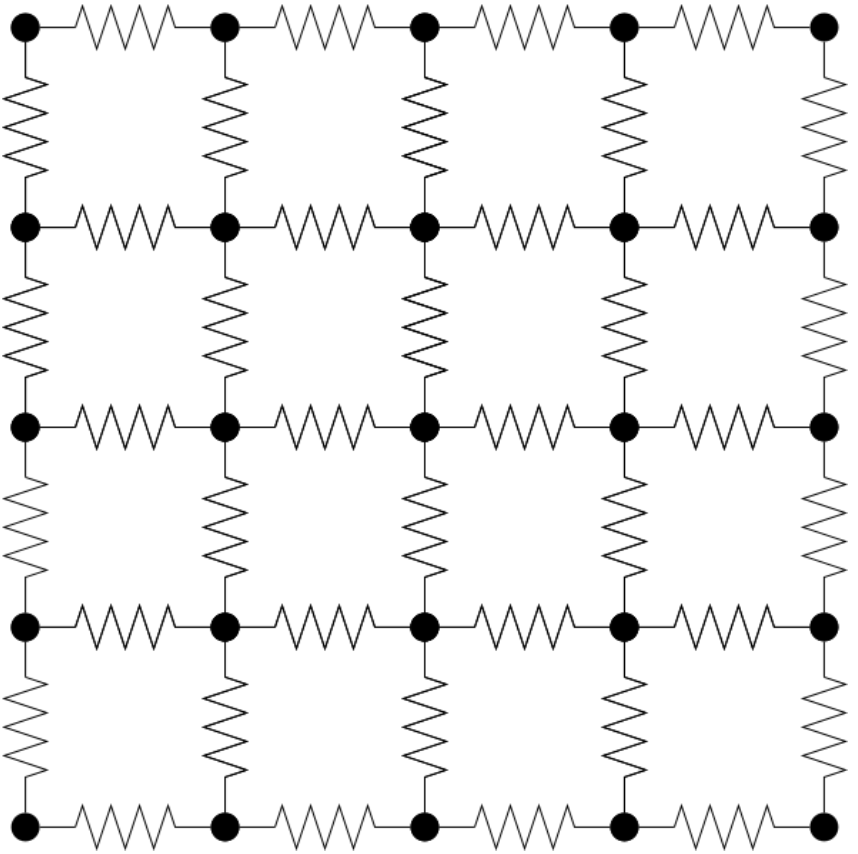
\includegraphics[width=\textwidth]{Ressort1.png} 
        \caption{Réseau de ressorts régulier}
        \label{fig:Ressort1}
    \end{subfigure}
    \hspace*{30pt}
    \begin{subfigure}[b]{0.3\textwidth}
        \centering
        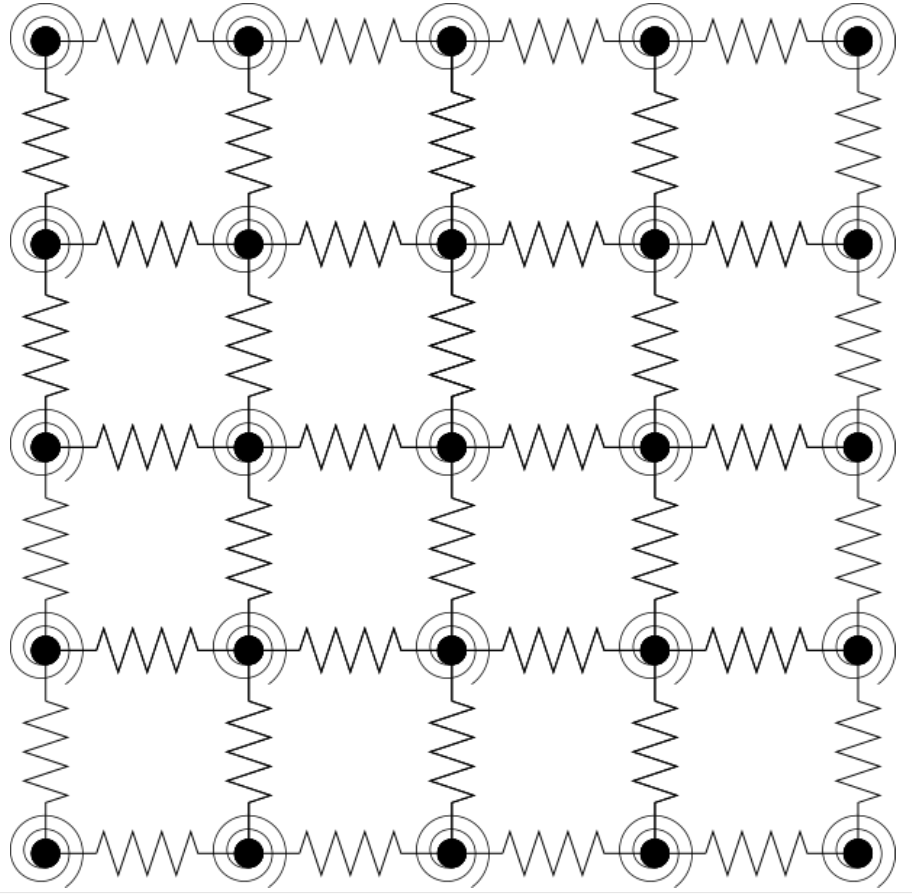
\includegraphics[width=\textwidth]{Ressort2.png} 
        \caption{Réseau de ressorts régulier avec torsion}
        \label{fig:Ressort2}
    \end{subfigure}
       \caption{Réseau de ressort considéré durant cette étude.}
       \label{fig:Reseau}
\end{figure}

Ensuite, \citeauthor{balasoiu2020halthesis} considère la suite $\tau_n$ de réseau défini, comme aux paragraphes précédents par :
$$
\tau_{n,0} = \Omega \cap \frac{1}{n} \mathbb{Z}^2 \,.
$$
On rappelle que $k_1$, $k_2$ représentent les constantes de raideurs des ressorts sur les arrêtes du réseau dans les deux directions de $\Omega$, et $G$ la constante de torsion des ressorts aux n\oe{}uds. Sur le maillage $\tau_n$, après définition des énergies redimensionnées élastiques de traction $R_n$, et de torsion $T_n$, \parencite[p.91]{balasoiu2020halthesis} montre les théorèmes ci-après. 

\begin{theorem}[$\Gamma$-convergence]
    \label{theo:gammaconv}
    La suite d'énergie redimensionnée $(E_n)_{n\in\mathbb{N}}$ $\Gamma$-converge, pour la topologie faible de $H^1(\Omega, \mathbb{R}^2)$, vers la fonctionnelle limite :
    \begin{align*}
        \eel : H^1(\Omega, \mathbb{R}^2) &\rightarrow \mathbb{R} \\
        &u \mapsto \frac{1}{2} \int_{\Omega} C_h e(u):e(u) \diff x \,,
    \end{align*}
    avec $C_h$ le tenseur de rigidité du matériau homogénéisé, qui vérifie, pour un tenseur $M$ d'ordre 2 :
    $$
    C_{h,ijkl}M:M = k_1 M^2_{1,1} + k_2 M^2_{2,2} + 16G(M_{1,2} + M_{2,1})^2 \,,
    $$
    De plus, ce tenseur est celui d’un matériau élastique homogène et isotrope si et seulement si l’on a $k_1 = k_2 = k = 8G$. Dans ce cas, on a :
    $$
    \eel(u) = \frac{1}{2} \int_{\Omega} K_{\lambda, \mu}e(u) : e(u) \diff x \,,
    $$
    avec :
    $\lambda = 0$, et $\mu = \frac{k}{2}$.
\end{theorem}


\begin{theorem}[Équi-coercivité]
    Soit $(\tau_n)_{n\in\mathbb{N}}$ une suite de maillages du plan, et $(u_n) \in \mathbb{N}$ une suite de déplacements admissibles de $H^1(\Omega, \mathbb{R}^2)$, i.e. vérifiant :
    $$
        \forall n \in \mathbb{N}, \quad u_n \in \wadm (\tau_n, \mathbb{R}^2) \,.
    $$
    On suppose de plus que cette suite de déplacement est bornée pour l’énergie :
    $$
    \exists C > 0 , \forall n \in \mathbb{N}, \quad E_{n}(u_n) \leq C \,.
    $$
    Alors la suite $(u_n)_{n \in \mathbb{N}}$ est bornée dans $H^1(\Omega, \mathbb{R}^2)$.
\end{theorem}
\noindent Le \cref{theo:gammaconv} permet de constater que le tenseur de rigidité obtenu, lorsqu’il est isotrope, a un coefficient de Poisson nul\footnote{Cela correspond par exemple à un étirement longitudinal du réseau de ressorts, sans effet (amincissement ou épaississement) sur la section transversale.}. \citeauthor{balasoiu2020halthesis} a donc proposé un calcul formel de la limite simple de la suite d’énergies discrètes dans le cas ou le réseau de ressorts serait stochastique et de loi isotrope. En particulier, il trouve dans ce cas un coefficient de Poisson fixe de $1/4$.


% %%------------------------------------------------------------------------------





\subsection{Un processus stochastique de maillages isotropes} 

\textit{Le résumé du chapitre \parencite[p.136]{balasoiu2020halthesis} est ici très succinct. Ce chapitre fait appel à des outils fins de probabilité conditionnelle et de processus stochastiques, telles que \textbf{mesure et formules de Campbell}, \textbf{distribution de Palm}, etc. }

Dans ce chapitre, \citeauthor{balasoiu2020halthesis} a construit un processus stochastique de maillage, qui à chaque tirage associe un maillage de Delaunay. Il commence par donner plusieurs formules de calcul, les deux formules de Campbell ainsi que la formule de Slivnyak-Mecke, qui permettent de calculer l’espérance d’une variable aléatoire qui s’écrit comme la somme d’une fonction en chaque point du maillage. Ces formules se montrerons très utiles pour le calcul de l’énergie élastique d’un réseau de ressorts basé sur ce processus de maillage.


\noindent La notion de processus ponctuel est un outil qui peut permettre de construire un ensemble de points dénombrable, sans point d'accumulation. \citeauthor{balasoiu2020halthesis} définit un \textbf{processus stochastique simple de $\mathbb{R}^d$} comme : une variable aléatoire $\Phi$ d’un espace de probabilités $(\Omega, \mathcal{A}, \mathbb{P})$ dans l’espace $(\mathfrak{N}, \mathcal{N})$. Elle induit une loi de probabilité $\mathbb{P}_\Phi$ sur $(\mathfrak{N}, \mathcal{N})$ : l’espace $(\mathfrak{N}, \mathcal{N}, \mathbb{P}_\Phi)$ est un espace de probabilités. Dans cette définition, nous avons:  
\begin{itemize}
    \item $\mathfrak{N}$ est ensemble des parties localement finies de $\mathbb{R}^d$. Autrement dit, il s'agit de l'ensemble des motifs de points de $\mathbb{R}^d$;
    \item $\mathcal{N}$ est la plus petite tribu (sur $\mathfrak{N}$) qui rende mesurable les applications qui comptent le nombre de points du processus. 
\end{itemize}
Une fois le processus défini, on peut définir sa \textbf{mesure d'intensité} $\Lambda(\cdot)$:
\begin{align*}    
    \Lambda : \mathcal{B}(\mathbb{R}^d) &\rightarrow \overline{\mathbb{R}}^+ \\
    B & \mapsto \mathbb{E}(\Phi(B)) = \mathbb{E}(\text{Card } \Phi \cap B) \,,
\end{align*}
où $\mathbb{E}(F)$ désigne l'espérance de la variable aléatoire $F:\mathfrak{N}\rightarrow \mathbb{R}$.

\noindent La première formule de Campbell permet de relier la moyenne d’une somme sur les points du processus avec l’intensité du processus. En effet, soit $f:\mathbb{R}^d \rightarrow \mathbb{R}$ une fonction mesurable et positive, on a :
$$
\mathbb{E} \left( \sum_{x \in \Phi} f(x) \right) = \int_{\mathbb{R}^d} f(x) \diff \Lambda(x) \,.
$$
Un processus stochastique ponctuel $\Phi$ est dit de Poisson (cf. \cref{fig:poisson}) s'il vérifie les hypothèses suivantes
: 
\begin{enumerate}
    \item $\Phi$ est à éparpillement indépendant, c’est-à-dire que si $(B_i)_{i \in {1,...,k}}$ sont des boréliens deux à deux disjoints ; alors les variables aléatoires $\Phi(B_i)$ sont indépendantes ;
    \item pour tout $B$ borélien, la variable aléatoire $\Phi(B) = \text{Card } (\Phi \cap B)$ suit une loi de Poisson de moyenne $\mu =  \lambda \nu_d(B)$ , c’est-à-dire que :
    \[
    \mathbb{P}(\Phi (B) = m) = \frac{\mu^m}{m!}\exp(-\mu) \,.
    \]
\end{enumerate}

\begin{figure}[!h]
    \centering
    
\includegraphics[width=.4\textwidth]{Poisson.png}\
    \caption{Tirages d’un processus de Poisson d’intensité $10$ sur le carré unité \parencite[p.137]{balasoiu2020halthesis}. En premier, le nombre de point est obtenu par une v.a. suivant une loi de Poisson d'espérence $10$. Ensuite les coordonnés des points sont obtenues par simulation de deux v.a. suivant des lois uniformes \parencite{keeler2018simu}.}
    \label{fig:poisson}
\end{figure}

\citeauthor{balasoiu2020halthesis} ne s'arête pas là. Il définit aussi les notions d'espace Polonais, mesure de comptage, et de convergence faible dièse. Ces notions sont importance vu la nécessité d'associer un point du processus ponctuel à une marque, i.e. un simplexe de $\mathbb{R}^d$ dans notre cas. \citeauthor{balasoiu2020halthesis} introduit la notion de mesure de Campbell, qui permet d'obtenir la seconde formule de Campbell. Ensuite il définit la distribution de Palm, permettant ainsi d'obtenir la très importante formule de Campbell-Mecke:
\[
\mathbb{E} \left( \sum_{x \in \Phi} f(x,\Phi) \right) = \int_{\mathbb{R}^d} \int_{\mathfrak{N}} f(x,\varphi) \diff
\mathbb{P}_x(\varphi) \diff \Lambda(x) \,.
\]
où $f:\mathbb{R}^d \times \mathfrak{N} \rightarrow \mathbb{R}$ est une fonction, mesurable et positive. Lorsque le processus ponctuel $\Phi$ est stationaire d'intensité $\lambda$, on a:
\[
 \int_{\mathfrak{N}} \sum_{x \in \varphi} f(x,\varphi_{ - x}) \diff\mathbb{P}_\Phi(\varphi) = \lambda \int_{\mathbb{R}^d} \int_{\mathfrak{N}} f(x,\varphi) \diff
\mathbb{P}_0(\varphi) \diff \Lambda(x) \,.
\]
où $\mathbb{P}_0$ désigne la distribution de Palm. Le résultat de Slynvyak-Mecke suivant est une généralisation de cette dernière formule, lorsque le processus $\Phi$ est de Poisson, et la fonction $f:(\mathbb{R}^d)^n \times \mathfrak{N} \rightarrow \mathbb{R}$ mesurable positive :
\[
\mathbb{E} \left( \sum_{x_1,\ldots,x_n \in \Phi} f(x_1,\ldots,x_n,\Phi) \right) = \frac{\lambda^n}{n!} \int_{(\mathbb{R}^d)^n} \mathbb{E} \left(f(x_1,\ldots,x_n,\Phi \cup \{ x_1,\ldots,x_n \}) \right) \diff x_1 \ldots \diff x_n \,.
\]

La prochaine étape consiste en la présentation d'un \textbf{théorème ergodique} qui lie la forme globale d’un seul tirage avec la forme moyenne en un point de plusieurs tirages. Ici aussi, \citeauthor{balasoiu2020halthesis} se base sur les travaux de D. J. Daley et D. Vere-Jones \parencite{daley2008introduction}.
\begin{theorem} \label{th:slmk}
    Soit $\Phi$ un processus de Poisson, et $f$ une fonction mesurable et positive qui vérifie :
    $$
    \mathbb{E}\left( \sum_{x\in \Phi} f(\Phi_{-x}) \right) < +\infty \,.
    $$
    On note $B_n$ la boule de $\mathbb{R}^d$, centrée en $0$ et de rayon $n$. On a presque sûrement la formule
    suivante :
    $$
    \lim_{n\rightarrow +\infty} \frac{1}{\Phi(B_n)} \sum_{x_i \in B_n \cap \Phi} f(\Phi_{-x_i}) = \int_{\mathfrak{N}} f(\varphi) \diff{\mathbb{P}_0(x)}  \,. 
    $$
\end{theorem}

Ensuite, \citeauthor{balasoiu2020halthesis} s'attaque aux notions de maillages et pavages, en particulier les \textbf{pavages de Voronoi} (cf. \cref{fig:vorodeloau}). Les maillages construits suivent une loi isotrope. En moyenne sur les tirages, toutes les directions des arêtes sont donc équitablement représentées. Un théorème ergodique permettra de transférer cette isotropie moyenne en isotropie presque sure si l’on dilate le maillage, autrement dit si on le regarde de suffisamment loin. 

\noindent Soit donc $\varphi \in \mathfrak{N}$ un ensemble localement fini de points. On appelle diagramme de Voronoi associé à $\varphi $ le pavage régulier de $\mathbb{R}^d$ par $(C(x))_{x\in \varphi}$, où la cellule $C(x)$ est définie par :
$$
C(x) = \left\{ y \in \mathbb{R}^d \, \big| \text{ dist }(y,x) < \inf_{z\in \varphi\backslash\{x\}}\text{ dist }(y,z) \right\} \,.
$$
\begin{figure}[H]
    \centering
    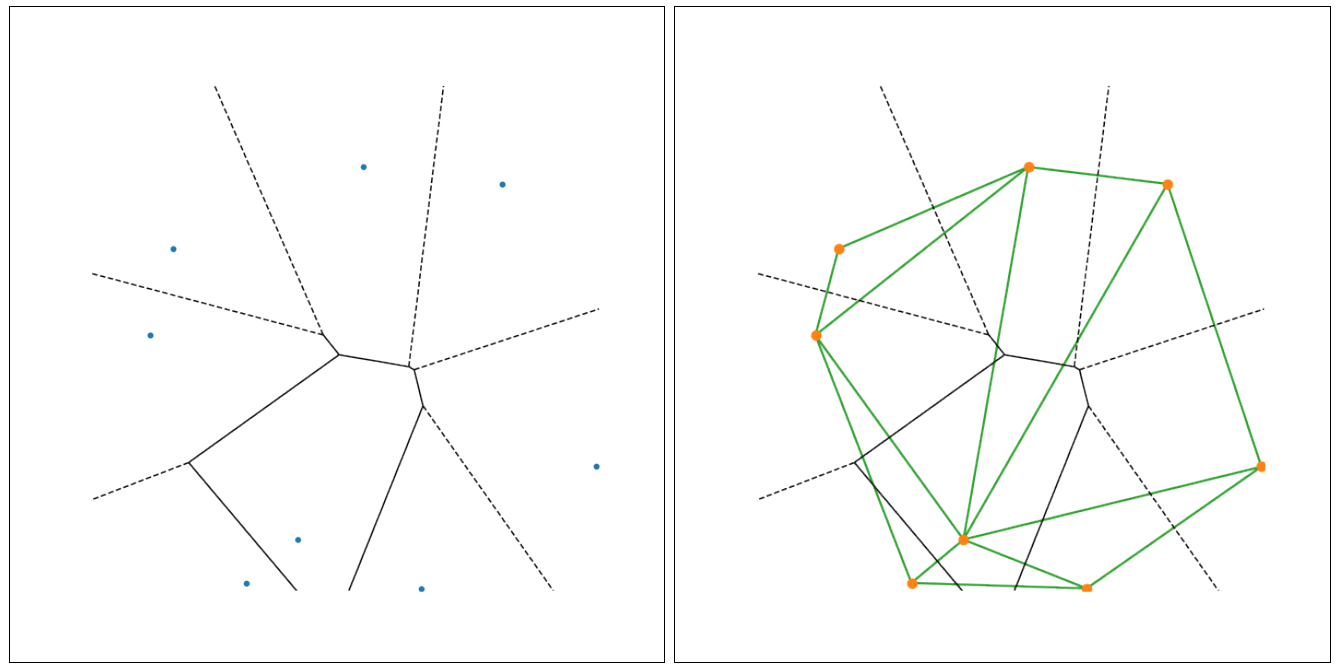
\includegraphics[width=.5\textwidth]{VoronoiDelaunay.png}\
    \caption{Ensemble de points avec les diagrammes de Voronoi (à gauche) et Delaunay (à droite) associés
    \parencite[p.138]{balasoiu2020halthesis}.}
    \label{fig:vorodeloau}
\end{figure}
\noindent En utilisant la formule de Slivnyak-Mecke (cf. \cref{th:slmk}), \citeauthor{balasoiu2020halthesis} montre que si $\Phi$ est un processus de Poisson, alors les points de $\varphi$ sont presque sûrement en \textbf{position générale}\footnote{Voir définition 4.4.5 de la thèse \parencite[p.128]{balasoiu2020halthesis}.}. En corolaire, si $\varphi$ est un ensemble de points en position générale, alors $\varphi$ est l’ensemble des sommets du \textbf{maillage de Delaunay}\footnote{Une triangularisation de Delaunay maximise le plus petit angle de l'ensemble des angles des triangles.} $D_\varphi$ construit sur le pavage de Voronoi $V_\varphi$.


Ce chapitre se termine par la notion de convergence d'une suite de maillages. \citeauthor{balasoiu2020halthesis} montre que, si l’on dilate (cf. \cref{fig:maillage}) le processus de Poisson-Delaunay initial et qu’on en restreint les réalisations à un domaine du plan, nous obtiendrons une suite de processus stochastiques dont les réalisations convergent presque sûrement vers le domaine fixé. Il a également donné un contrôle asymptotique de la taille minimale des mailles obtenues dans cette suite de processus de maillages. Ce contrôle sera utile dans la section suivante, pour calibrer le redimensionnement utilisé pour traduire l’hypothèse des petits déplacements sur le réseau de ressorts. 

\noindent Soit donc $D \subset \mathbb{R}^d$ un domaine, i.e. un ouvert connexe, de l’espace. Soit $\Phi$ un processus ponctuel de l’espace qui suit une loi de Poisson d’intensité $1$. Soit $(\lambda_n )_{n\in N} \subset \mathbb{R}^{+}$ une suite positive, croissante et divergente. On définit, pour tout entier $n \in \mathbb{N}$, le processus ponctuel $\Phi_n$ par :
$$
\Phi_n = \frac{1}{\sqrt[d]{\lambda_n}}\Phi \,.
$$
On note $\tau_n$ (cf. \cref{fig:maillage}) le maillage par simplexe définit presque sûrement comme la triangulation de Delaunay du nuage de points $\Phi_n \cap D$ :
$$\tau_n = \Theta_{\Phi_n \cap D} \,, $$
ce qui permet d'obtenir le théorème suivant :
\begin{theorem} \label{th:lambda}
    Si la suite d’intensités $(\lambda_n)_{n \in \mathbb{N}}$ vérifie :
    $$\exists k \in \mathbb{N}^\ast , \quad n^{1/k} = o(\lambda_n)\,,$$
    alors, presque sûrement, la suite $(\tau_n)_{n \in \mathbb{N}}$ de maillages de $D$ converge uniformément vers $D$.
\end{theorem}
\begin{figure}[H]
    \centering
    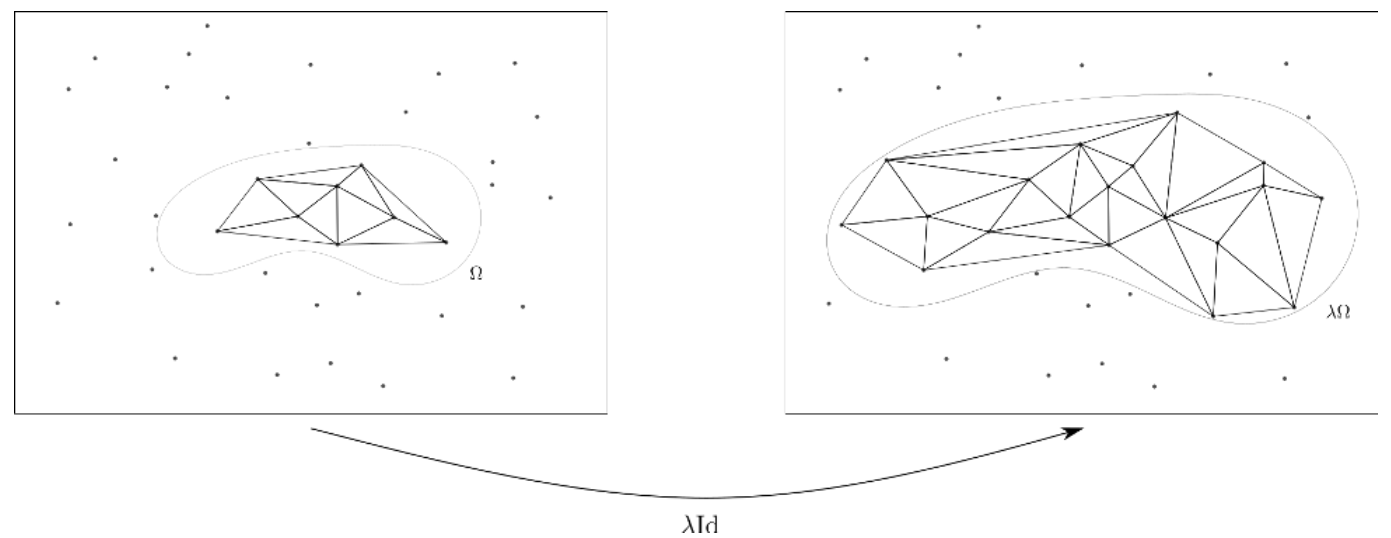
\includegraphics[width=.8\textwidth]{Maillage.png}\
    \caption{Dilatation de l'ouvert $D$ \parencite[p.138]{balasoiu2020halthesis}.}
    \label{fig:maillage}
\end{figure}





\subsection{Étude asymptotique d’un réseau de ressorts isotrope} 

Dans cette partie, \citeauthor{balasoiu2020halthesis} propose un second résultat d’approximation d’un matériau élastique par un réseau de ressorts. Dans la partie précédente, il avait proposé un résultat d’approximation d’un matériau élastique par un réseau régulier, à mailles carrées. Ici, les mailles seront triangulaires. Plus précisément Le réseau de ressorts que nous utiliserons dans ce chapitre est défini dans la section précédente, et repose sur la théorie des processus stochastiques ponctuels.
Nous proposons dans ce chapitre un résultat de $\Gamma$-convergence de l’énergie élastique sur un réseau de ressorts, issu d’un processus stochastique de loi isotrope. 

Présentons le réseau de ressorts utilisé pour approcher l’énergie élastique d’un matériau continu $D$. Il s'agit des mêmes définitions utilisées pour introduire le \cref{th:lambda} ci-haut, cette fois ci \textbf{en dimension $2$}. On suppose que $D \subset \mathbb{R}^2$ est un domaine du plan, i.e. un ouvert du plan, qui est connexe et dont la frontière est lisse. On considère une triangulation quelconque $\tau$ du domaine $D$. On note $W (\tau, \mathbb{R}^2)$ l’espace des éléments finis $P1$ défini sur le maillage $\tau$. On note, comme précédemment, $ \wadm(\tau, \Rdeux)$ l’ensemble des déplacements admissibles :
$$
\wadm(\tau, \Rdeux) =  \left\{ u\in W(\tau, \Rdeux) \, \big| \, \forall w \in \tau_2, \forall q_1, q_2 \in \tau_0 \cap \overline{\omega}, q_1 \neq q_2, \quad q_1 + u(q_1) \neq q_2 + u(q_2)  \right\} \,.
$$
On souhaite construire un réseau de ressorts sur $\tau$ tel que l’énergie totale $E_\tau$ soit équi-coercive. Mais puisque l’on utilisera des triangulations construites sur un processus de Poisson, la coercivité n'est pas assurée. Pour remédier à ce manque de coercivité, on va placer sur $\tau$ deux types de ressorts : des \textbf{ressorts de traction} et des \textbf{ressorts de torsion}. Les constantes de raideur des ressorts de traction et de torsion dépendent des angles du triangle de base des ressorts, et elles tendent vers l’infini si l’angle correspondant tend vers $0$. Les constantes de rigidité des réseaux de ressorts sont supposées constantes. On note, comme aux sections précédents, $R_\tau$ l’énergie du réseau de ressorts de traction, et $T_\tau$ l’énergie du
réseau de ressorts de torsion. On note de plus :
$$ E_\tau = R_\tau + T_\tau \,, $$
l’énergie totale sur le réseau $\tau$. On note également, pour tout triangle $t \in \tau_2$ du maillage, $\nu_1$ , $\nu_2$ et $\nu_3$ ses trois cotés, ainsi que $\theta_1$, $\theta_2$ et $\theta_3$ les trois angles opposés (voir \cref{fig:triangle}).

\begin{figure}[!h]
    \begin{subfigure}{0.45\textwidth}
        \centering
        \frame{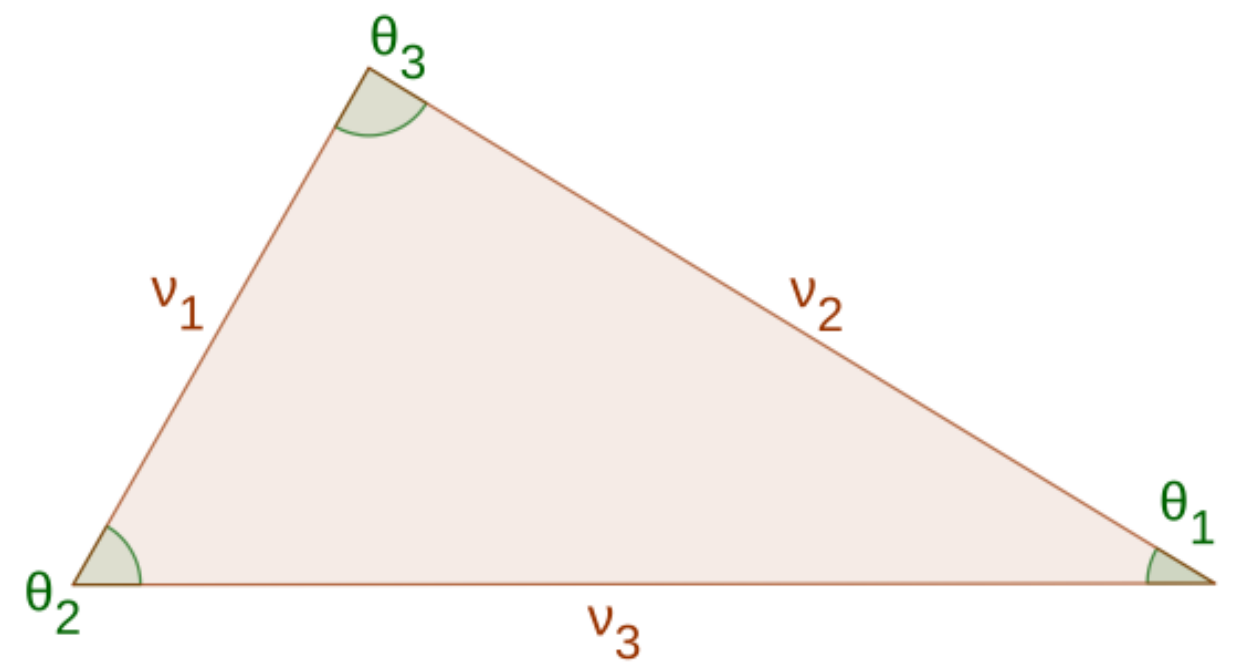
\includegraphics[width=\textwidth]{Triangle.png}}
        \caption{Triangle du maillage \parencite[p.184]{balasoiu2020halthesis}.}
        \label{fig:triangle}
    \end{subfigure}
    % \hfill
    \begin{subfigure}{0.3\textwidth}
        \centering
        \frame{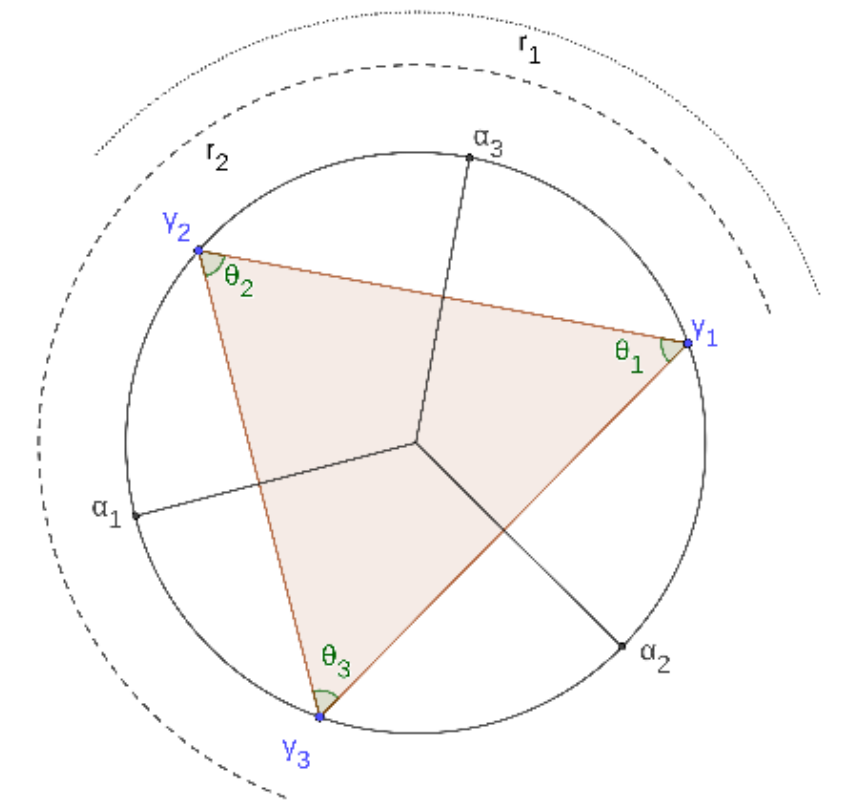
\includegraphics[width=\textwidth]{ChangementVar.png}}
        \caption{Changement de variables dans un triangle \parencite[p.184]{balasoiu2020halthesis}.}
        \label{fig:changement}
    \end{subfigure}
    \caption{Illustration des eléments du maillages, et des coodonnées.}
\end{figure}

\begin{figure}[H]
    \centering
    \frame{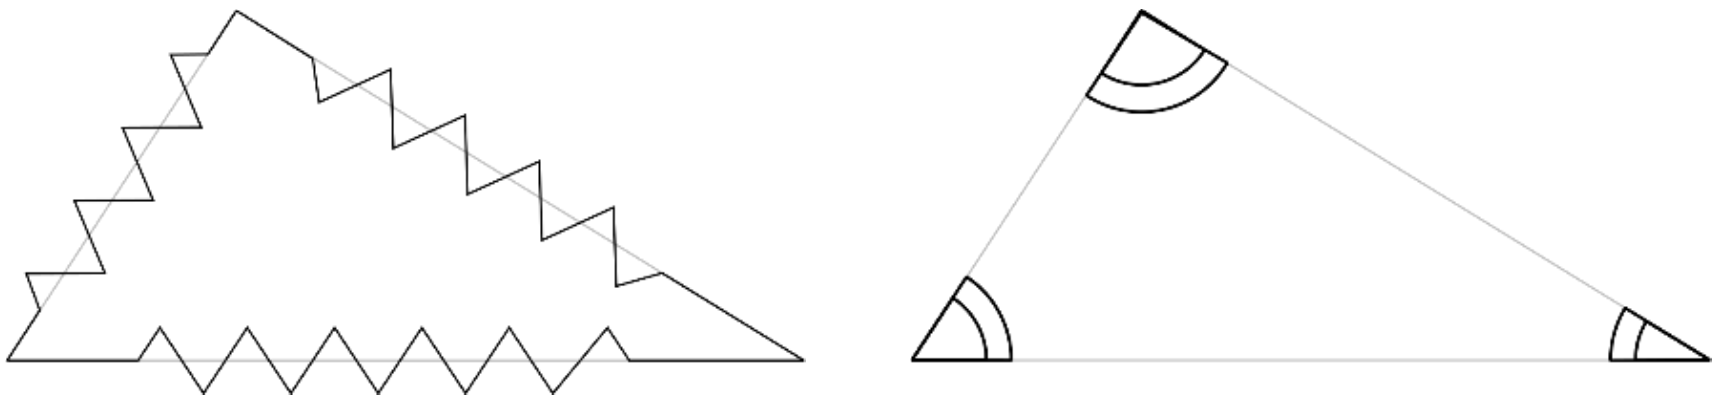
\includegraphics[width=.8\textwidth]{Ressorts.png}}
    \caption{Ressorts de traction (à gauche) et de torsion (à droite) \parencite[p.184]{balasoiu2020halthesis}.}
    \label{fig:ressorts}
\end{figure}

On commence par définir l’énergie élastique du réseau de ressorts de traction $R_\tau$, et on renvoie à la \cref{fig:ressorts}. On note $k > 0$ la constante de rigidité du réseau. On place, sur chaque arête $\nu_i$ de chaque triangle $t$ du maillage, un ressort de traction de longueur à vide $l_i = \vert \nu_i \vert$ et de raideur $k_i$, avec :
$$
\forall i \in \mathbb{Z}/3\mathbb{Z}, \quad k_i = \frac{k}{\sin(\theta_i)} \,.
$$
Si $\varphi \in W (\tau, \Rdeux)$ est une déformation du réseau de ressort, et $u = \varphi -
\identity$ est le déplacement associé, l’énergie élastique discrète de l’assemblage vaut :
$$
R_{\tau}(u) = \sum_{t\in \tau_2} \sum_{i=1}^{3} \frac{k \vert \nu_i \vert^2}{2 \sin(\theta_i)} \left( \Vert \nabla \varphi e_{\nu_i} \Vert - 1 \right)^2 \,.
$$
On définit maintenant l’énergie $T_\tau$, et on renvoie aux \cref{fig:ressorts,fig:changement}.
On note $G > 0$ la constante de rigidité de torsion du réseau. On place, sur chaque angle
$\theta_i$ de chaque triangle $t$ du maillage, un ressort de torsion de raideur $G_i$ :
$$
\forall i \in \mathbb{Z}/3\mathbb{Z}, \quad G_i = \frac{G \vert\nu_{i+1} \vert \, \vert\nu_{i+2}
    \vert}{\sin(\theta_i)} \,.
$$
On définit l’énergie élastique discrète de l’assemblage :
$$
T_\tau (u) = \sum_{t\in \tau_2} \sum_{i=1}^{3} \frac{G \vert\nu_{i+1} \vert \vert\nu_{i+2} \vert}{2\sin(\theta_i)} \left(  \angle(\varphi(\nu_{i+1}), \varphi (\nu_{i+2})) - \angle(\nu_{i+1},\nu_{i+2}) \right)^2 \,,
$$
avec $\angle(\cdot,\cdot)$ l’angle entre deux vecteurs du plan.
Ensuite, on étend les énergies élastiques définies sur les réseaux à $H^1(D, \Rdeux)$, en notant:
\begin{align*}
    R_\tau: H^1(D, \Rdeux) &\rightarrow \Run  && T_\tau:
    H^1(D, \Rdeux )  \rightarrow \Run \\
    u &\mapsto \begin{dcases}
        R_\tau (u) \text{ si } u \in W(\tau,\Rdeux) \,, \\
        +\infty \text{ sinon } \,,
    \end{dcases}
    && \qquad \qquad \quad \,\, \, u \mapsto \begin{dcases}
        T_\tau (u) \text{ si } u \in \wadm(\tau,\Rdeux) \,, \\
        +\infty \text{ sinon } .
    \end{dcases}
\end{align*}
On définit maintenant la suite d’énergies élastiques définies sur la suite des réseaux
$(\tau_n)_{n \in \mathbb{N}}$. On introduit un changement d’échelle des énergies
$(E_{\tau_n})_{n \in \mathbb{N}}$ pour prendre en compte
l’hypothèse des petits déplacements. Soit $(\varepsilon_n)_{n \in \mathbb{N}}$ une suite
positive qui tend vers $0$. On note, pour tout entier $n \in \mathbb{N}$ :
\begin{align*}
    R_\tau: H^1(D, \Rdeux) &\rightarrow \Run  && T_\tau:
    H^1(D, \Rdeux )  \rightarrow \Run \\
    u &\mapsto \varepsilon_n^{-2} R_{\tau_n}(\varepsilon_n u)\,,
    && \qquad \qquad \quad \,\, \, u \mapsto \varepsilon_n^{-2} T_{\tau_n}(\varepsilon_n u)\,,
\end{align*}
et on pose: $$ E_n = R_n + T_n. $$
On donne enfin une version modifiée des suites de fonctionnelles $(E_n)_{n \in \mathbb{N}}$ et $(T_n)
_{n \in \mathbb{N}}$ qui prenne en compte une condition de Dirichlet sur le bord de $D$. Soit donc
$v \in \text{ Lip}(\Rdeux, \Rdeux)$ la donnée du bord. On note :
$$
W_n^v(\tau, \Rdeux) =  \left\{ u\in \wadm(\tau, \Rdeux) \, \big| \, \forall p \in \tau_0, \text{
    dist }(p,\partial D) \leq \lambda_n, \, \, u(p) = v(p)\, \right\}.
$$
On pose ensuite, pour tout entier $n \in \mathbb{N}$ :
\begin{align*}
    R_\tau^v: H^1(D, \Rdeux) &\rightarrow \Run  && T_\tau^v:
    H^1(D, \Rdeux )  \rightarrow \Run \\
    u &\mapsto \begin{dcases}
        R_\tau (u) \text{ si } u \in W_n^v(\tau_n,\Rdeux) \,, \\
        +\infty \text{ sinon } \,,
    \end{dcases}
    && \qquad \qquad \quad \,\, \, u \mapsto \begin{dcases}
        T_\tau (u) \text{ si } u \in W_n^v(\tau_n,\Rdeux) \,, \\
        +\infty \text{ sinon } \,,
    \end{dcases}
\end{align*}
ainsi que $$ E_n^v = R_n^v + T_n^v \,. $$

On énonce à présent les trois théorèmes principaux du chapitre.
\begin{theorem}[Convergence simple]
    On a presque sûrement la propriété suivante. Pour  toute fonction $u \in C^1(D, \Rdeux)$, il
    existe une suite de déplacements discrets $(u_n)_{n \in \mathbb{N}}$ admissibles, i.e. :
    $$\forall n \in \mathbb{N}, \quad u_n \in \wadm (\tau_n, \Rdeux) \,,$$
    et qui vérifie de plus :
    $$\forall u \in  C^1 (D, \Rdeux), \quad E_n(u_n) \underset{n \rightarrow +\infty}
    \longrightarrow E_s(u)\, $$
    avec :
    $$ E_s(u) = \int_{D} K_{\lambda,\mu} e(u):e(u) \diff x \,, $$
    où $K_{\lambda,\mu}$ est le tenseur de Lamé du matériau, qui vérifie :
    $$ \forall e \in M_2(\Run), \quad K_{\lambda,\mu} e: e = \lambda \text{ \upshape tr}(e)^2 + 2 \mu \text{ \upshape tr}(e)^2 \,, $$
    avec $\lambda$ et $\mu$ respectivement les première et deuxième constantes de Lamé, qui valent :
    $$ \lambda = \frac{32 k \vert A \vert}{9 \pi^2} + \frac{3G \vert A \vert}{4}\,, \quad \mu =
    \frac{32 k \vert A \vert}{9 \pi^2} - \frac{3G \vert A \vert}{4}. $$
\end{theorem}

\begin{theorem}[$\Gamma$-convergence]
    Supposons que la suite de changements d’échelle $(\varepsilon_n)_{n \in \mathbb{N}}$ vérifie :
    \[ \exists \alpha > 0, \quad \varepsilon_n = o\left(  \frac{1}{\lambda_n n^{1/2 + \alpha}}
    \right) \,. \]
    Alors, la suite de fonctionnelles redimensionnées $(E_n)_{n \in \mathbb{N}}$ $\,
    \Gamma$-converge
    presque sûrement vers la fonctionnelle $E_{\text{\upshape hom}} : L^2(D, \Rdeux) \rightarrow
    \mathbb{R}^+$ définie  par :
    \begin{align*}
        E_{\text{\upshape hom}}(u)  =
        \begin{dcases}
                          \int_{D} K_{\lambda_h,\mu_h} e(u):e(u) \diff x &\quad \text{      \upshape si } u \in H^1(D,
                          \Rdeux) \,, \\
                          + \infty &\quad  \text{      \upshape sinon }\,,
        \end{dcases}
    \end{align*}
    où $K_{\lambda,\mu}$ est le tenseur de Lamé du matériau, qui vérifie :
    \[\forall e \in M_2(\Run), \quad K_{\lambda_h,\mu_h} e: e = \lambda_h \text{ \upshape tr}(e)^2 + 2 \mu_h \text{ \upshape tr}(e)^2 \,. \]
    De plus, pour toute donnée au bord $v$ dans $\text{  \upshape Lip}(\Rdeux, \Rdeux)$, la suite de
    fonctionnelles $(E^v_n)_{n \in \mathbb{N}}$ $\, \Gamma$-converge presque sûrement vers la
    fonctionnelle  $E^v_{\hom} : L^2(D, \Rdeux) \rightarrow \mathbb{R}^+ $ définie par :
    \begin{align*}
        E^v_{\text{\upshape hom}}(u)  =  \begin{dcases}
                          \int_D K_{\lambda_h,\mu_h} e(u):e(u) \diff x &\quad \text{  \upshape si } u - v \in
                          H^1(D,
                          \Rdeux) \,, \\
                          + \infty &\quad \text{  \upshape sinon }\,.
        \end{dcases}
    \end{align*}
\end{theorem}

\begin{theorem}[Équi-coercivité]
    Soit $(E_n)_{n \in \mathbb{N}}$ une suite de maillages du plan et $(u_n)_{n \in \mathbb{N}}$
    une suite de déplacements admissibles de $H^1(\Omega, \Rdeux)$, i.e. vérifiant :
    $$\forall n \in \mathbb{N}, u_n \in \wadm (\tau_n, \mathbb{R}^2) \,.$$
    On suppose de plus que cette suite de déplacements est bornée pour l’énergie :
    $$ \exists C > 0\,, \forall n \in \mathbb{N}, \quad E_n(u_n) \leq C \,. $$
    Alors la suite $(u_n)_{n \in \mathbb{N}}$ est bornée dans $H^1(\Omega, \Rdeux)$.
\end{theorem}





\subsection{Résultat de quasi-staticité à grande raideur} 
\label{subsubsec:chap6dimitri}


Ce dernier chapitre propose un résultat de quasi-staticité d’un réseau de ressorts percuté par un objet ponctuel lorsque la raideur du système et sa masse totale tendent vers l’infini. Lors de la collision de floes de glaces, la vitesse relative des floes (de l’ordre de grandeur de la dizaine de centimètres par seconde, voir \parencite{rampal2009arctic}) est bien inférieure à la vitesse de propagation des ondes élastiques dans la glace (de l’ordre de grandeur de $1800$ mètres par seconde pour les ondes de cisaillement, voir \parencite{marsan2019characterizing}). \citeauthor{balasoiu2020halthesis} montre que, lors de la percussion d’un réseau masse-ressort par un objet solide, les effets dynamiques disparaissent lorsque la raideur des ressorts tend vers l’infini. Autrement dit, nous montrons que le réseau limite, de raideur infinie, est à chaque instant dans un état d’équilibre. Plus précisément, nous observerons que le système différentiel qui modélise la percussion s’écrit comme le couplage de deux sous-systèmes. Le premier, dit \textbf{système intérieur} (SI), est à évolution rapide et modélise la propagation des ondes élastiques dans le système masse-ressort. Le second, dit \textbf{système extérieur} (SE), est à évolution lente et modélise la pénétration de l’objet solide dans le système masse-ressorts.

On étudie le phénomène de percussion d’un système masse-ressort de $n + 1$ particules, chacune de masse $m$, par un objet ponctuel $P$ de masse $M$. Le système masse-ressort utilisé est de constante de raideur $k>0$, et de constante de viscosité $\mu>0$. Soit $\tau \in \mathcal{T} (\Rdeux)$ une triangulation compacte et connexe du plan. En chaque n\oe{}ud $q \in \tau_0$, on place une masse ponctuelle $m$. Sur chaque arête $\omega \in \tau_1$ de $\tau$, on place en parallèle (voir \cref{fig:masseressort}) :
\begin{enumerate}
    \item un ressort de longueur à l’équilibre $L_0$ et de raideur $k$,\
    \item un dissipateur visqueux, de viscosité $\mu$.
\end{enumerate}
\begin{figure}[!h]
    \centering
    \frame{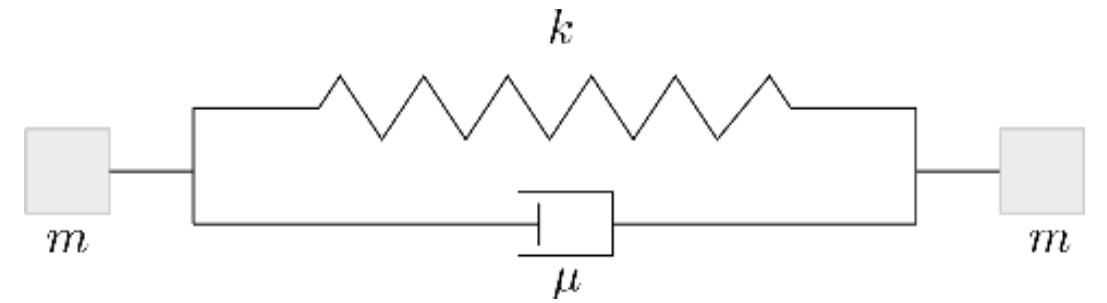
\includegraphics[width=0.5\textwidth]{MasseRessort.png}}
    \caption{Système élémentaire masse-ressort utilisé.}
    \label{fig:masseressort}
\end{figure}
On suppose qu’à l’instant $t = 0$, le système masse-ressorts est à l’équilibre, et qu’il est percuté par la masse ponctuelle $P$ au point $q_0 \in \partial\tau_0$. On note $v_0$ la vitesse du point $P$ lors de la collision. On suppose également que le système $\{q_0, P\}$ \textbf{devient inséparable}, de masse $m + M$.
Sur le maillage $\tau$ , on note $\tau_0$ l’ensemble des n\oe{}uds du système. On a donc :
$$\tau_0 = \{\bvec q_0, . . . , \bvec q_n \} \,,$$ où les $\bvec q_i$ sont les coordonnées des masses. On rappelle que le système est à l’équilibre au temps $t = 0$. On note $a, b \in \mathcal{M}_{2,n+1} (\Run)$ les vecteurs de positions et vitesses initiales définis
par :
$$
\begin{cases}
    a = (\bvec q_0(0), \ldots, \bvec q_n(0)) \,, \\
    b = (\bvec v_0,0,\ldots,0) \,.
\end{cases}
$$
On note de plus $C \in \mathcal{M}_{n+1}(\Run)$ la matrice de connectivité :
$$
∀0 \leq i < j \leq n + 1, C_{i,j} = C_{j,i} =
\begin{cases}
    1 \text{ si } q_i \in \mathcal{V}(\bvec q_j) \,, \\
    0 \text{ sinon },
\end{cases}
$$
où $\mathcal{V}(q)$ désigne l’ensemble des voisins de la particule $q \in \tau_0$. On note encore $L_{ij} \in \mathcal{M}_{n+1} (\Run)$ la matrice des longueurs à l’équilibre dont l’expression est déduite de $\tau_0$; et $\bvec{u}_{ij}$ le vecteur unitaire (s'il existe) dans la direction de l'arête entre $\bvec q_i$ et $\bvec q_j$. On obtient le système différentiel suivant en appliquant l'équation d'Euler-Newton sur les moments linéaires, et en exprimant la force de frottement du dispositif visqueux en fonction de $\dot q$ :
\begin{align} \tag{$E$} \label{eq:e}
\begin{dcases}
    \bvec{\ddot{q}}_0 = \sum_{j=0}^{n}C_{0j} \left[  \frac{k}{M+m} \left( \Vert \bvec{q}_j - \bvec{q}_0 \Vert - L_{0j} \right) \bvec{u}_{0j} -\frac{\mu}{M+m} \left\langle \bvec{\dot{q}}_j - \bvec{\dot{q}}_0\,, \bvec{u}_{0j}  \right\rangle  \bvec{u}_{0j}  \right] \,, &\qquad \text{(SE)} \\
    \bvec{\ddot{q}}_i = \sum_{j=0}^{n}C_{ij} \left[  \frac{k}{m} \left( \Vert \bvec{q}_j - \bvec{q}_i \Vert - L_{ij} \right) \bvec{u}_{ij} -\frac{\mu}{m} \left\langle \bvec{\dot{q}}_j - \bvec{\dot{q}}_i\,, \bvec{u}_{ij}  \right\rangle  \bvec{u}_{ij}  \right]  \quad \forall 1 \leq i \leq n \,. &\qquad \text{(SI)}
\end{dcases}
\end{align}
D'un point de vue énergétique, on a la loi de conservation de l'énergie suivante:
\begin{align*}
    \eel(t) + E_{\text{c}}(t) + E_{\text{r}}(t) = E_0 \,,
\end{align*}
où $\eel(t), \,, E_{\text{c}}$, et $E_{\text{r}}$ désignent respectivement l'énergie élastique du système, l'énergie cinétique, et l'énergie dissipée par les frottements visqueux \parencite[p.188]{balasoiu2020halthesis}. $E_0$ désigne l'énergie initiale du système donnée par :
$$
E_0 = \frac{1}{2}(M+m)\Vert \bvec{v}_0 \Vert^2 \,.
$$
Sous ces hypothèses et ces définitions, \citeauthor{balasoiu2020halthesis} obtient le théorème d'existence globale ci=après.
\begin{theorem}[Existence d'une solution globale] \label{th:solglob}
    On suppose que les conditions initiales adjointes au système d'\cref{eq:e} vérifient la condition énergétique :
    $$
    E_0 < \frac{k}{4} \left( \inf_{\omega \in \tau_1} \vert \omega \vert \right)^2 \,.
    $$
    Alors, le problème de Cauchy est bien posé\footnote{Le système est bien posé si deux particules voisines restent à une distance $c > 0$ l’une de l’autre.} et ses solutions sont globales.
\end{theorem}

Ensuite, afin d'obtenir un système à grande raideur et de supprimer les perturbations liées à la propagation des ondes élastiques, \citeauthor{balasoiu2020halthesis} introduit une dépendance en $\varepsilon$ des constantes physiques du système : $k_\varepsilon$ , $M_\varepsilon$ et $\mu_\varepsilon$. En posant :
$$
k_\varepsilon = \frac{k}{\varepsilon} \,, \quad M_\varepsilon = \frac{M}{\varepsilon^2} , \quad \mu_\varepsilon = \frac{\mu}{\varepsilon} \,,
$$
le système masse-ressort se réécrit :
\begin{align} \tag{$E_{\varepsilon}$} \label{eq:eeps}
\begin{dcases}
    \bvec{\ddot{q}}_0 = \sum_{j=0}^{n}C_{0j} \left[  \frac{k}{M+\varepsilon^2 m} \left( \Vert \bvec{q}_j - \bvec{q}_0 \Vert - L_{0j} \right) \bvec{u}_{0j} - \varepsilon\frac{\mu}{M+\varepsilon^2 m} \left\langle \bvec{\dot{q}}_j - \bvec{\dot{q}}_0\,, \bvec{u}_{0j}  \right\rangle  \bvec{u}_{0j}  \right] \,, \\
    \varepsilon^2 \bvec{\ddot{q}}_i = \sum_{j=0}^{n}C_{ij} \left[  \frac{k}{m} \left( \Vert \bvec{q}_j - \bvec{q}_i \Vert - L_{ij} \right) \bvec{u}_{ij} - \varepsilon \frac{\mu}{m} \left\langle \bvec{\dot{q}}_j - \bvec{\dot{q}}_i\,, \bvec{u}_{ij}  \right\rangle  \bvec{u}_{ij}  \right]  \quad \forall 1 \leq i \leq n \,. 
\end{dcases}
\end{align}
On écrit également le système limite :
\begin{align} \tag{$E_{lim}$} \label{eq:elim}
\begin{dcases}
    \bvec{\ddot{q}}_0 = \sum_{j=0}^{n}C_{0j}  \frac{k}{M} \left( \Vert \bvec{q}_j - \bvec{q}_0 \Vert - L_{0j} \right) \bvec{u}_{0j} \,, \\
    \bvec{0} = \sum_{j=0}^{n}C_{ij} \frac{k}{m} \left( \Vert \bvec{q}_j - \bvec{q}_i \Vert - L_{ij} \right) \bvec{u}_{ij} \, \quad \forall 1 \leq i \leq n \,.
\end{dcases}
\end{align}
Ce problème est un problème de perturbation singulière, pour lequel \citeauthor{balasoiu2020halthesis} prouve le théorème de limite quasi-statique ci-bas (en se servant principalement du théorème classique de A.N.Tikhonov \parencite{tikhonov1952systems,hoppensteadt1966singular}).
\begin{theorem}[Limite quasi-statique]
    Les solutions $ \bvec q_\varepsilon$ et $\bvec q$ respectivement des systèmes perturbé \cref{eq:eeps} et limite \cref{eq:elim} munis des conditions initales\footnote{Des conditions initiales satisfaisant le \cref{th:solglob}.} existent, sont uniques et globales.
    De plus, on a :
    $$
    \lim_{\varepsilon \rightarrow 0} \bvec q_{\varepsilon}(t) = \bvec q(t) \,, \quad \forall t \in \mathbb{R}^+ \,.
    $$
\end{theorem}

Du point de vue numérique, les simulations ont permis de comprendre l’influence des différents paramètres physiques présents (masse des deux objets, raideur des ressorts, vitesse d’impact etc.). De plus, le code Python et HTML/CSS développé fournira une bonne base pour analyser la localisation des vecteurs propres du système dynamique et identifier ceux qui agissent sur un déplacement du bord. Présentons le principal résultat numérique utilisé. À $\varepsilon > 0$ fixé, on note $(\lambda_i (\varepsilon))_{i \in \{0,...,4n+3\}}$ les valeurs propres de l’opérateur associé à la linéarisation du système \cref{eq:eeps} autour de sa position d’équilibre, et on les ordonne ainsi:
$$
0 \geq \mathfrak{R}(\lambda_8(\varepsilon)) \geq \mathfrak{R}(\lambda_9(\varepsilon)) \geq \ldots \geq \mathfrak{R}(\lambda_{4n+3}(\varepsilon)) \,.
$$
Nous définissons le saut spectral $\nu_{\varepsilon}$ associé au système (\ref{eq:eeps}) de la manière suivante :
$$
\nu_{\varepsilon} = \frac{\mathfrak{R}(\lambda_{12}(\varepsilon))}{\mathfrak{R}(\lambda_{11}(\varepsilon))} \,.
$$
Ce saut représente l’écart entre les quatre premières valeurs propres non nulles du système, qui correspondent au système lent (SE), et la première valeur propre du système rapide (SI). Après avoir tracé le saut spectral $\nu_{\epsilon}$ pour différentes triangulations $\tau$ (cf. \cref{fig:res3} pour un exemple), \citeauthor{balasoiu2020halthesis} constate qu'il s'agit de droites dont les pentes ne dépendent ni du tirage, ni de l’intensité du processus de Poisson-Delaunay. Il propose donc l’expression suivante pour $\nu_{\varepsilon}$ :
$$
\ln(\nu_{\varepsilon}) = a_0(\tau) + \alpha \ln(\varepsilon) \,,
$$
avec $a_0 (\tau)$ une quantité qui dépend du maillage $\tau$, et $\alpha$ une constante universelle, indépendante de $\tau$ et $\varepsilon$ numériquement estimée à la valeur :
$$\alpha = −2 \pm 10^{−3} \,.$$
La \cref{fig:res2} ci-dessous a été obtenue, pour un processus de Poisson-Delaunay d’intensité $500 000$, l’histogramme de la valeur de $a_0$ associée sur $1 000$ tirages.
\begin{figure}[!h]
    \centering
    \begin{subfigure}{0.29\textwidth}
        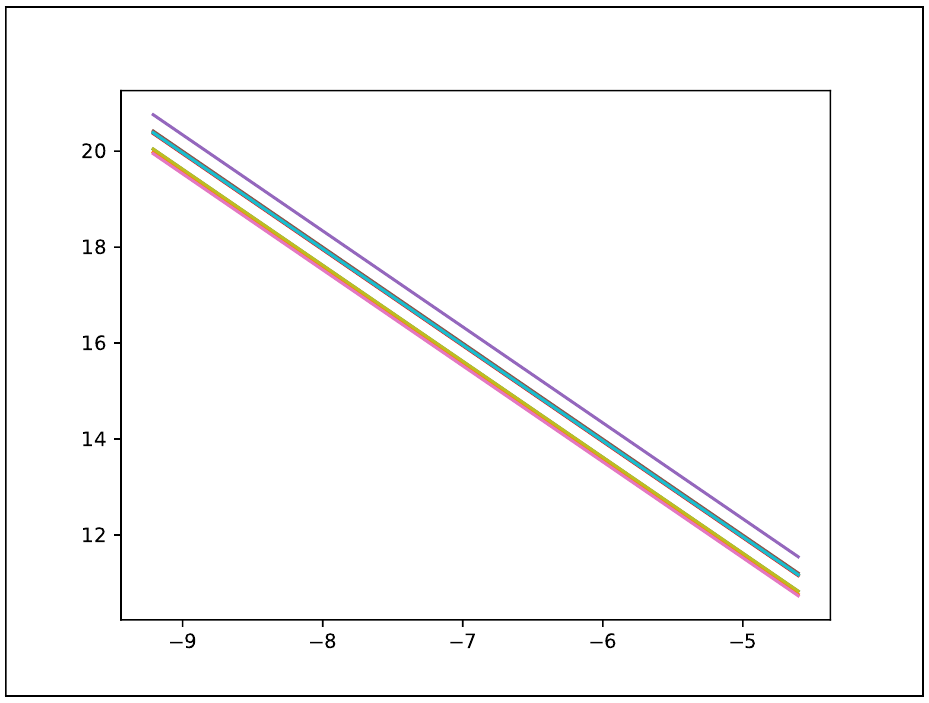
\includegraphics[width=\textwidth]{Res3.png}
        \caption{}
%        \caption{Saut spectral en fonction de la perturbation, en échelle log-log, sur dix tirages d’un processus de Poisson-Delaunay d’intensité $1000$.}
        \label{fig:res3}
    \end{subfigure}
    \begin{subfigure}{0.3\textwidth}
        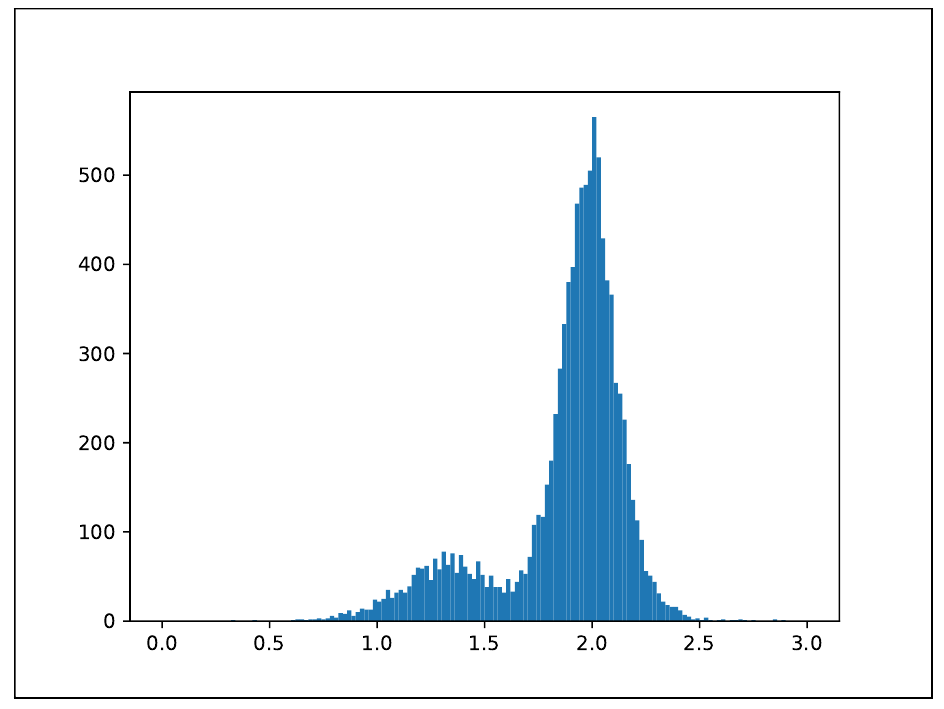
\includegraphics[width=\textwidth]{Res1.png}
        \caption{}
%        \caption{Histogrammes du paramètre $a_0$, sur $10 000$ tirages d’un processus de Poisson-Delaunay d’intensité $2500$.}
    \end{subfigure}
    \begin{subfigure}{0.3\textwidth}
        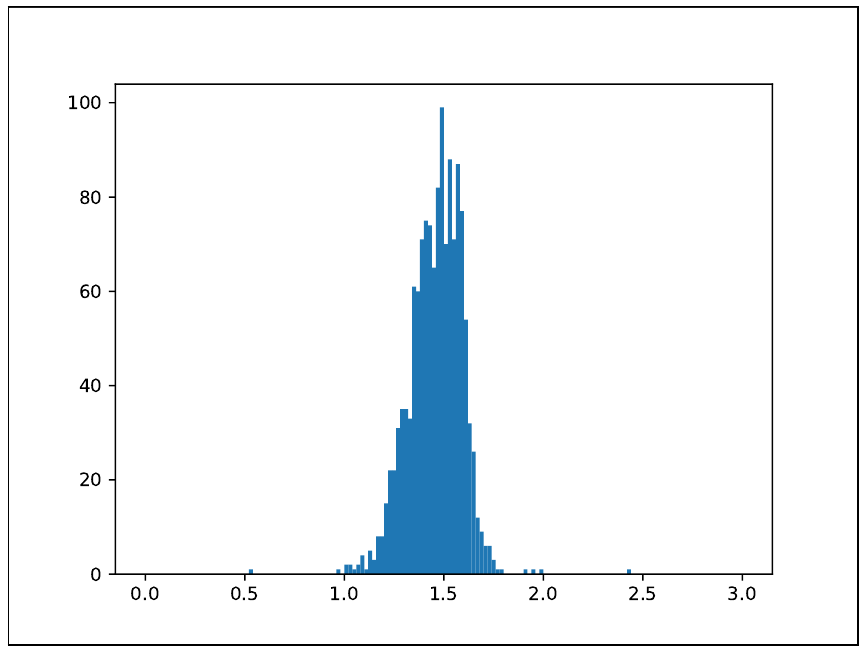
\includegraphics[width=\textwidth]{Res2.png}
        \caption{}
%        \caption{Histogramme du paramètre $a_0$ sur $1 000$ tirages d’un processus de Poisson-Delaunay d’intensité $500 000$}
        \label{fig:res2}
    \end{subfigure}
    % \decoRule
    \caption{Principaux résultats numériques obtenus \parencite[p.199]{balasoiu2020halthesis}. \textbf{(a)}: saut spectral en fonction de la perturbation, en échelle log-log, sur dix tirages d’un processus de Poisson-Delaunay d’intensité $1000$. \textbf{(b)}: histogrammes du paramètre $a_0$, sur $10 000$ tirages d’un processus de Poisson-Delaunay d’intensité $2500$. \textbf{(c)}: histogramme du paramètre $a_0$ sur $1 000$ tirages d’un processus de Poisson-Delaunay d’intensité $500 000$.}
\end{figure}
\noindent Ces résultats semblent indiquer, à grande échelle au moins, que $a_0(\tau)$ prend ses valeurs entre $0.9$ et $2.5$. Nous observons également l’émergence de deux pics pour certaines intensités. Il semblerait que le pic de valeur moyenne la plus faible gagne en fréquence de représentation, jusqu'à concentrer la quasi-totalité des cas pour l’intensité de $500 000$.




\subsection{Discussion et questions ouvertes}

Plusieurs hypothèses sont faites dans la thèse pour limiter la complexité du modèle. Ces simplifications sont à l'origine de simplifications que nous précisions ci bas :
\begin{enumerate}
    \item Le modèle suppose que les floes sont d’épaisseur négligeable devant leur extension horizontale ; autrement dit, les déformations du floe de glace peuvent être étudiées en deux dimensions.
    \item Le modèle restreint l’ensemble des fractures admissibles à celui des segments de droites \parencite[chp.2]{balasoiu2020halthesis}.
    \item Au chapitre 6 \parencite[p.187]{balasoiu2020halthesis}, il serait également intéressant d’intégrer, comme dans les chapitres 3, 4, et 5, des ressorts de torsion en chaque n\oe{}ud du système masse-ressort \parencite[p.187]{balasoiu2020halthesis}.
    \item Au chapitre 5 \citeauthor[p.183]{balasoiu2020halthesis}, \citeauthor{balasoiu2020halthesis} a montré que la suite d’énergies élastiques $\Gamma$-converge vers une énergie limite. De plus, lorsque le redimensionnement est suffisamment rapide, il a montré que la $\Gamma$-limite s’écrit comme l’énergie d’un matériau élastique homogène et isotrope, soumis à l’hypothèse des petits déplacements. Cette énergie dépend donc de deux paramètres, les deux constantes de Lamé du matériau homogénéisé. Il serait intéressant d’adapter l’étude numérique \parencite{ostoja1995linear} pour obtenir une expression des constantes de Lamé homogénéisées dans notre cas.
    \item Il reste, à l’issue de la thèse, d'obtenir une seconde limite spatiale. Cette limite est une limite de couche, qui indiquerait l’expression du déplacement au bord du floe lors de la percussion. Nous pourrions l’obtenir en sélectionnant les vecteurs propres du système dynamique masse-ressorts qui influent sur le comportement d’une couche mince du bord du floe \parencite[p.201]
    {balasoiu2020halthesis}.
    \item Dans une prochaine étude, on pourrait étudier la percussion du système masse-ressort par un objet solide non ponctuel et qui ne serait pas fixé au système étudié. \citeauthor{balasoiu2020halthesis} pense que le cas général peut se déduire du cas étudié au chapitre 6 \parencite[p.187]{balasoiu2020halthesis}. En effet, l’étude de la percussion complète reviendrait à ajouter, dans le système différentiel étudié, un nombre fini de perturbations singulières à des instants distincts. 
\end{enumerate}











%%4----------------------------------------------------------------------------------------

\section{Résumé de l'état de l'art}

En résumé, nous constatons que Rabatel et Balasoiu ont fondamentalement posés les bases du travail que nous allons effectuer durant ce stage. Dans sa thèse, Rabatel s'est focalisé sur l'étude de la dérive des floes de glace dans la mer. Le puissant modèle qu'il a développé a pu être testé et validé sur des floes de glace en bassins, avec de données climatiques provenant d'\textbf{ERAinterim} et \textbf{TOPAZ}. Cependant, il a considéré les floes de glace comme des objets solides ne pouvant se briser, ce qui n'est pas le cas dans la nature. 

C'est pour résoudre le problème de fracture que Balasoiu a considéré, dans sa thèse, les floes de glace comme un assemblage discrets de masses reliés par des ressorts à grandes raideurs et des dispositifs visqueux. Il a dans un premier temps étudié la nucléation et la propagation de la fracture dans un matériau élastique soumis à un chargement quasi-statique \footnote{Balasoiu extraira, dans une seconde partie, une limite temporelle qui montre qu'un réseau limite de raideur infinie est, à chaque instant, dans un état d’équilibre; ce qui justifie l’hypothèse de quasi-staticité du phénomène de percussion.}. Balasoiu s'est ensuite penché sur la percussion d'un matériau élastique. Il a pour ceci considéré le floe comme un réseau de ressorts \footnote{Il justifie cette bonne approximation en exhibant une première limite spatiale.} et a étudié le résultat de la collision entièrement élastique d'un objet ponctuel avec un floe, au niveau d'un des n\oe{}ud de ce dernier. Au terme de son travail, Balasoiu propose d'exhiber une deuxième limite spatiale, celle permettant de dériver de l’équation différentielle du système entier l’expression du déplacement au bord du floe. 

Notre travail va consister en l'étude du phénomène de percussion de plus près. Nous extrairons les déplacements des n\oe{}uds des floes (et sur le bord en particulier) après une collision, et nous étudierons, à travers le modèle de Griffith et sa compétition entre les énergies de déformation et de fracture, dans quelles circonstances la fracture apparait. Nous étudierons tout ceci à l'aide de simulations précises écrites en Python en 1D, et de 2D. 



       %% Environnement économique du stage
% 
% Chapter 3

\chapter{État de l'art} % 3rd chapter title

\label{Chapter3} % For referencing the chapter elsewhere, use \ref{Chapter3} 


% %----------------------------------------------------------------------------------------

% \section{Position du problème}
% \label{sec:position}

% Nous commençons par présenter une modélisation mathématique d'une plaque de glace (appelé floe) sur la mer. Six variables (locales) sont nécessaires pour décrire le floe occupant la région fermée de l'espace $\Omega$ (voir \cref{fig:floe}) :
% \begin{itemize}
%     \item Un ouvert connexe $\omega \in \Rdeux$ décrivant la section longitudinale du floe ;
%     \item Deux fonctions $\hplus, \hmoins \in \mathcal{F}(\omega, \Run)$ décrivant l'épaisseur du floe, telle que $\forall x \in \omega, \hmoins(x) \leq \hplus(x)$ ;
%     \item Le centre de masse du floe $G(w)$ ;
%     \item Deux vecteurs $\eun$ et $\edeux$ formant une base sur $\omega$.
% \end{itemize}

% \begin{figure}[!ht]
%     \centering
%     \begin{subfigure}[b]{0.35\textwidth}
%         \centering
%         % 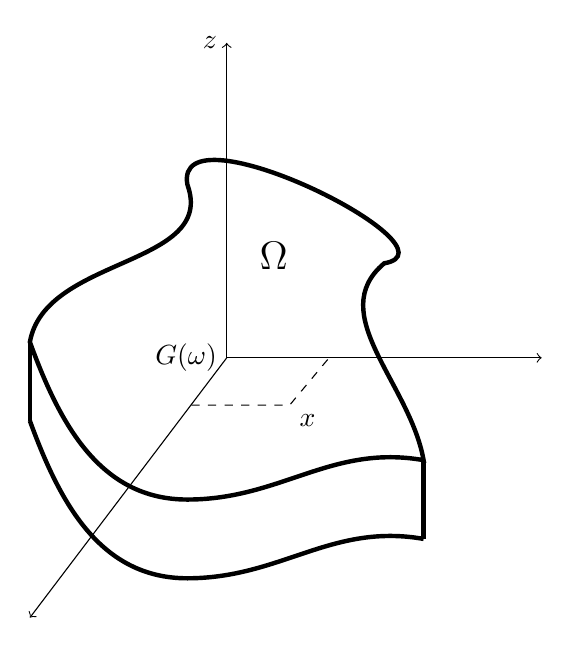
\begin{tikzpicture}
\node[coordinate] (v1) at (-3,3) {};
\node[coordinate] (v2) at (-5,1) {};
\node[coordinate] (v3) at (-3,-1) {};
\node[coordinate] (v4) at (0,-0.5) {};
\node[coordinate] (v5) at (-0.5,2) {};
%\draw  plot[smooth cycle, tension=.7] coordinates {(v5) (v1) (v2) (v3) (v4) (v5)};

\draw [ultra thick] (v1) to [out=290, in=80] (v2) to[out=290, in=180] (v3) to[out=0,in=170] (v4) to[out=100,in=220] (v5) to[out=10,in=100] (v1);

\node[coordinate] (v6) at (-5,0) {};
\node[coordinate] (v7) at (-3,-2) {};
\node[coordinate] (v8) at (0,-1.5) {};

\draw [ultra thick] (v2)--(v6); \draw [ultra thick] (v4)--(v8);
\draw [ultra thick]  (v6) to[out=290, in=180] (v7) to[out=0,in=170] (v8);

\node[coordinate] (v9) at (-2.5,0.8) {};
\node[coordinate] (v10) at (-5.0,-2.5) {};
\node[coordinate] (v11) at (1.5,0.8) {};
\node[coordinate] (v12) at (-2.5,4.8) {};

\draw [->] (v9)--(v10);
\draw [->] (v9)--(v11);
\draw [->] (v9)--(v12);


\node[left] (v9) at (-2.5,0.8) {$G(\omega)$};
\node[left] (v12) at (-2.5,4.8) {$z$};
\node[above left] (v13) at (-1.6,1.8) {\Large $\Omega$};

\node[coordinate] (v14) at (-1.2,0.8) {};
\node[coordinate] (v15) at (-1.7,0.2) {};
\node[coordinate] (v16) at (-2.95,0.2) {};
\draw[dashed] (v16)--(v15)--(v14);

\node[below right] (v15) at (-1.7,0.2) {$x$};

\end{tikzpicture}
%         \includegraphics[width=.8\textwidth]{FloeVue1.tikz} 
%         \caption{Vue d'un floe}
%         \label{fig:floe1}
%     \end{subfigure}
%     % \hfill
%     \begin{subfigure}[b]{0.35\textwidth}
%         \centering
%         % \usetikzlibrary{patterns}

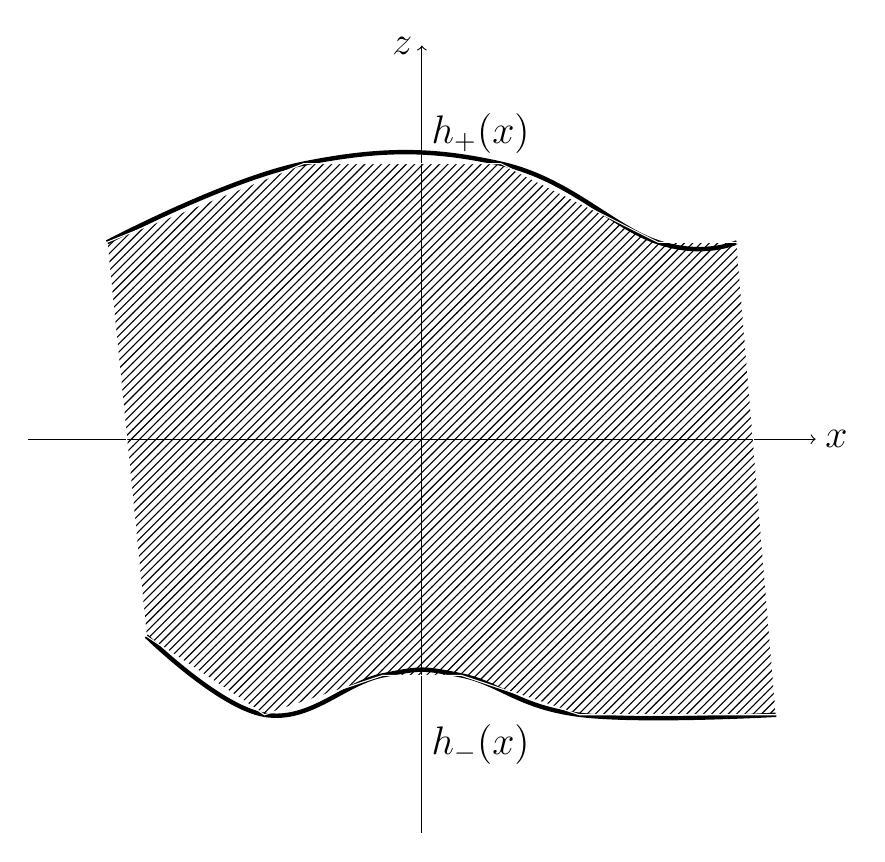
\begin{tikzpicture}

\node[coordinate] (v0) at (0,0) {};
\node[coordinate] (v1) at (-5,0) {};
\node[coordinate] (v2) at (5,0) {};
\node[coordinate] (v3) at (0,-5) {};
\node[coordinate] (v4) at (0,5) {};

\draw [->] (v1)--(v2);
\draw [->] (v3)--(v4);

\node (v5) at (-4,2.5) {};
\node (v6) at (-1.5,3.5) {};
\node (v7) at (1,3.5) {};
\node (v8) at (3,2.5) {};
\node (v9) at (4,2.5) {};
\node (v10) at (-3.5,-2.5) {};
\node (v11) at (-2,-3.5) {};
\node (v12) at (-0.5,-3) {};
\node (v13) at (0.5,-3) {};
\node (v14) at (2,-3.5) {};
\node (v15) at (4.5,-3.5) {};

\draw[ultra thick]  plot[smooth, tension=.7] coordinates {(v5) (v6) (v7) (v8) (v9)};
\draw[ultra thick]  plot[smooth, tension=.7] coordinates {(v10) (v11) (v12) (v13) (v14) (v15)};

\draw [white, pattern=north east lines, xshift=0.5cm,yshift=4.5cm] plot coordinates {(v5) (v6) (v7) (v8) (v9) (v15) (v14) (v13) (v12) (v11) (v10) (v5)};

\node [above right] at (0,3.5) {\Large \bfseries $h_{+}(x)$};
\node [below right] at (0,-3.5) {\Large \bfseries $h_{-}(x)$};
\node [right] at (5,0) {\Large \bfseries $x$};
\node [left] at (0,5) {\Large \bfseries $z$};

\end{tikzpicture} 
%         \includegraphics[width=.8\textwidth]{FloeVue2.tikz} 
%         % \includegraphics[width=2cm]{Figures/FloeVue2.tex}
%         \caption{Coupe transversale}
%         \label{fig:floe2}
%     \end{subfigure}
%        \caption{Illustration de la géométrie d'un floe de glace $\Omega$.}
%        \label{fig:floe}
% \end{figure}

% \noindent On confond le floe au volume qu'il occupe dans l'espace $\Omega$ :
% \[
%     \Omega = \{(x,z) \,|\, x \in \omega \in \Rdeux, \, z \in \,]\hmoins(x), \hplus(x)[ \, \} \,.
% \] 
% Les fonctions $\hmoins$ et $\hplus$ permettent de définir trois quantités (voir \cref{fig:h}) :
% \begin{itemize}
%     \item L'épaisseur moyenne du floe : $\bar{h} =  \sup_{x\in\omega}{\hplus(x)} - \inf_{x\in\omega}{\hmoins(x)}$ ;
%     \item La plus forte épaisseur : $\bar{h}^* = \sup_{x\in\omega}{ \vert \hplus(x) - \hmoins(x) \vert}$ ;
%     \item La plus faible épaisseur : $\underline{h}^* = \inf_{x\in\omega}{ \vert \hplus(x) - \hmoins(x) \vert}$. 
% \end{itemize}

% \begin{figure}[!ht]
%     \centering
%     % \begin{tikzpicture}
	\begin{pgfonlayer}{nodelayer}
		\node [style=none] (0) at (0, 0) {};
		\node [style=none] (1) at (0, 5) {};
		\node [style=none] (2) at (0, -5) {};
		\node [style=none] (3) at (10, 0) {};
		\node [style=none] (4) at (-10, 0) {};
		\node [style=none] (5) at (-9.25, 2.5) {};
		\node [style=none] (6) at (-3.5, 1.5) {};
		\node [style=none] (7) at (3.25, 1.25) {};
		\node [style=none] (8) at (8.75, 4.75) {};
		\node [style=none] (9) at (-9, -6.75) {};
		\node [style=none] (10) at (-5, -4) {};
		\node [style=none] (11) at (2.5, -1.75) {};
		\node [style=none] (12) at (8.75, -1.25) {};
	\end{pgfonlayer}
	\begin{pgfonlayer}{edgelayer}
		\draw [->] (1.center) to (2.center);
		\draw [->] (4.center) to (3.center);
		\draw [bend right=15, looseness=0.75] (5.center) to (6.center);
		\draw [in=-165, out=0, looseness=1.25] (6.center) to (7.center);
		\draw [in=-135, out=15, looseness=1.25] (7.center) to (8.center);
		\draw [in=-165, out=45] (9.center) to (10.center);
		\draw [in=195, out=0, looseness=0.50] (10.center) to (11.center);
		\draw [in=180, out=15, looseness=0.75] (11.center) to (12.center);
	\end{pgfonlayer}
\end{tikzpicture}

%     \includegraphics[width=.6\textwidth]{h.tikz}
%     \caption{Différentes épaisseurs décrivant un floe de glace. Pour l'instant, afin d'obtenir un floe relativement plat (i.e $\bar{h}$ faible), $\hmoins$ sera pris identiquement nul, et $\hplus$ constant.}
%     \label{fig:h}
% \end{figure}

% \noindent Les vecteurs $\eun$ et $\edeux$ sont liés à $\omega$, et pointent vers un point fixe du bord $\partial \omega$ du floe c-à-d :
% \[
%     \exists \sigma_i \in \partial \omega \, | \, e_i(\omega) = \frac{\sigma_i - G(\omega)}{\Vert \sigma_i - G(\omega) \Vert}, \text{ pour } i \in \{1,2\} \,,
% \]
% où $\Vert \cdot \Vert$ désigne la norme euclidienne de $\Rdeux$. Notons que $\sigma_1 \neq \sigma_2$, et $\eun \cdot \edeux = 0$ de façon à ce que la base orthonormée $(\eun, \edeux)$ soit directe.

% Un floe $\Omega = (\omega, \eun, \edeux, G(\omega), \hmoins, \hplus)$ se déplace sur la mer\footnote{Pour l'instant, la mer est considérée comme un ouvert dans $\Rdeux$. Plus tard, nous prendrons en compte sont épaisseur lorsque nous la modéliserons par une sphère de $\Rtrois$.} $\mathcal{M} \in \Rdeux$. Au temps $t$ après une translation de vecteur $u(t)$ (et de matrice $\mathsf{T}_{u(t)}$), et une rotation de vecteur $\theta(t)$ (et de matrice $\bmat{R}_{\theta(t)}$), on obtient le floe $\Omega (t)$ défini par :
% \[
%     \Omega (t) = (\omega^\prime, \bvec e^1(\omega^\prime), \bvec e^2(\omega^\prime), G(\omega^\prime), \hmoins, \hplus) \,,
% \]
% avec
% $$ 
% \begin{cases}
%     \omega^\prime = \bmat{T}_{u(t)} \bmat{R}_{\theta(t)} \omega \,, \\
%     \bvec e_1(\omega^\prime) = \bmat{T}_{u(t)} \bmat{R}_{\theta(t)} \bvec e_1(\omega) \,, \\
%     \bvec e_2(\omega^\prime) = \bmat{T}_{u(t)} \bmat{R}_{\theta(t)} \bvec e_2(\omega) \,, \\
%     G(\omega^\prime) = \bmat{T}_{u(t)} \bmat{R}_{\theta(t)} G(\omega) \,.
% \end{cases}
% $$
% C'est cette dernière notation mettant en exergue la dépendance avec le temps que nous utiliserons tout au long de ce rapport.

% % \begin{figure}[!h]
% %     \centering
% %     % \begin{tikzpicture}
	\begin{pgfonlayer}{nodelayer}
		\node [style=none] (0) at (0, 0) {};
		\node [style=none] (1) at (0, 5) {};
		\node [style=none] (2) at (0, -5) {};
		\node [style=none] (3) at (10, 0) {};
		\node [style=none] (4) at (-10, 0) {};
		\node [style=none] (5) at (-9.25, 2.5) {};
		\node [style=none] (6) at (-3.5, 1.5) {};
		\node [style=none] (7) at (3.25, 1.25) {};
		\node [style=none] (8) at (8.75, 4.75) {};
		\node [style=none] (9) at (-9, -6.75) {};
		\node [style=none] (10) at (-5, -4) {};
		\node [style=none] (11) at (2.5, -1.75) {};
		\node [style=none] (12) at (8.75, -1.25) {};
	\end{pgfonlayer}
	\begin{pgfonlayer}{edgelayer}
		\draw [->] (1.center) to (2.center);
		\draw [->] (4.center) to (3.center);
		\draw [bend right=15, looseness=0.75] (5.center) to (6.center);
		\draw [in=-165, out=0, looseness=1.25] (6.center) to (7.center);
		\draw [in=-135, out=15, looseness=1.25] (7.center) to (8.center);
		\draw [in=-165, out=45] (9.center) to (10.center);
		\draw [in=195, out=0, looseness=0.50] (10.center) to (11.center);
		\draw [in=180, out=15, looseness=0.75] (11.center) to (12.center);
	\end{pgfonlayer}
\end{tikzpicture}

% %     \includegraphics[width=.4\textwidth]{FloeMer.tikz}
% %     \caption{Illustration du mouvement d'un floe de glace $F$ dans la mer, après une translation de vecteur $u(t)$ et une rotation d'angle $\theta(t)$, pour obtenir le floe $F_t$. On observe la transformation des propriétés du floe, en partucilier les vecteurs $e_1(\omega)$ et $e_2(\omega)$ qui restent liés au floe.}
% % \end{figure}


% Lors de leur mouvements sur la surface de la mer, les floes se fracturent sous l'effet des vents et des courants océaniques, des phénomènes thermodynamiques, etc. Nous nous intéresserons donc au phénomène de percussion en vue de l'initialisation des fractures dans les floes de glace. Afin de décrire le mouvement des floes de glace sur la mer, nous devons nous munir d'un repère absolu, que nous notons $\mathcal{R}_{abs} = (O, \bvec i, \bvec j, \bvec k)$. Le repère associé au floe $\Omega_i$ sera noté $\mathcal{R}_{\Omega_i} = (O, \bm \eun, \bvec \edeux, \bvec k)$. Dans ce repère absolu, le floe possède 3 degrés de libertés : l'abscisse et l'ordonné de son centre de gravité $G_i(\omega)$, et son orientation donnée par l'angle $\theta_i (t)$ (voir \cref{fig:FloeRepere}). 

% \begin{figure}[!ht]
%     \centering
%     % \begin{tikzpicture}
	\begin{pgfonlayer}{nodelayer}
		\node [style=none] (0) at (0, 0) {};
		\node [style=none] (1) at (0, 5) {};
		\node [style=none] (2) at (0, -5) {};
		\node [style=none] (3) at (10, 0) {};
		\node [style=none] (4) at (-10, 0) {};
		\node [style=none] (5) at (-9.25, 2.5) {};
		\node [style=none] (6) at (-3.5, 1.5) {};
		\node [style=none] (7) at (3.25, 1.25) {};
		\node [style=none] (8) at (8.75, 4.75) {};
		\node [style=none] (9) at (-9, -6.75) {};
		\node [style=none] (10) at (-5, -4) {};
		\node [style=none] (11) at (2.5, -1.75) {};
		\node [style=none] (12) at (8.75, -1.25) {};
	\end{pgfonlayer}
	\begin{pgfonlayer}{edgelayer}
		\draw [->] (1.center) to (2.center);
		\draw [->] (4.center) to (3.center);
		\draw [bend right=15, looseness=0.75] (5.center) to (6.center);
		\draw [in=-165, out=0, looseness=1.25] (6.center) to (7.center);
		\draw [in=-135, out=15, looseness=1.25] (7.center) to (8.center);
		\draw [in=-165, out=45] (9.center) to (10.center);
		\draw [in=195, out=0, looseness=0.50] (10.center) to (11.center);
		\draw [in=180, out=15, looseness=0.75] (11.center) to (12.center);
	\end{pgfonlayer}
\end{tikzpicture}

%     \includegraphics[width=.5\textwidth]{FloeRepere.tikz}
%     \caption{Positionnement d'un floe de glace $\Omega_i$ dans le repère absolu $\mathcal{R}_{abs}$.}
%     \label{fig:FloeRepere}
% \end{figure}


% %----------------------------------------------------------------------------------------

% \section{Résumé de thèse de M. Rabatel}

% Une fois le modèle défini, il nous faut établir les équations décrivant la dynamique du floe, et celle de son environnement. Les travaux de \citeauthor{rabatel2015thesis} (et plus tard ceux de \citeauthor{balasoiu2020thesis}) ont extensivement traité le problème de modélisation dynamique et de simulation d'un assemblage de floe de glace. Nous résumons ici les principales idées de son raisonnement, tout en présentant l'état de l'art dans ce domaine.

% \subsection{Modélisation théorique de la dynamique des glaces de mer}

% \subsubsection{La cinétique du floe}

% L'approche discrète décrite dans \parencite{rabatel2015thesis} utilise les mêmes notations que celles présentées à la \cref{sec:position}. Les obstacles\footnote{Nous faisons allusion aux obstacles au déplacement des floes. Il peut s'agir des iles, des stations offshore, etc.} sont des floes aux mêmes propriétés que les floes de glace, à la seule différence qu'ils ont une masse (volumique) infinie. Dans \parencite{rabatel2015thesis}, l'auteur travaille dans un repère orthonormé direct $\mathcal{R}_{abs} = (O, \bvec i, \bvec j, \bvec k)$ ; cependant, vu que la mer est considérée plane, le mouvement du floe peut être décrit dans le plan $\mathcal{P} = (O, \bvec i, \bvec j)$. Ensuite, \citeauthor{rabatel2015thesis} désigne la vitesse angulaire du floe $\Omega_i$ par 
% $$
% \bvec{\uptheta}_i(t) = \theta_i(t)\bvec{k} = (0,0,\theta_i(t))^T \,.
% $$
% Soit $P$ (de coordonné $x$) un point quelconque de $\P \subset \Rdeux$. Sa vitesse dans le repère $\R_{abs}$ est donnée est donnée par la formule de Varignon :
% $$
% \dot{P}(t) = \dot{G}_i(t) + \bm{\uptheta}_i(t) \wedge \bvec{G_iP} \,,
% $$
% où le symbole $\wedge$ représente le produit vectoriel dans $\Rtrois$. La masse (constante) du floe rigide indéformable est donnée par 
% $$
% M_i = \rho_i \int_{\Omega_i(t)} h_{i, +} (x) \diff x \,.
% $$
% Ensuite, l'auteur défini :
% \begin{itemize}
%     \item la somme des forces par unité de volume qui s'applique au centre de masse du floe $\Omega_i$ : $$\bvec{F}_i = \rho_i \int_{\Omega_i(t)} \bvec{F}(x) \diff x \,,$$
%     \item le moment cinétique\footnote{Il s'agit d'un moment dû à l'accélération du floe ; alors que le moment dynamique est dû aux forces extérieures. Notons que ces deux vecteurs sont portés par $\bvec{k}$, et peuvent donc être remplacé par des scalaires correspondants.} en $G$ : $$L_i = \rho_i \intO{i} \bvec{GP} \wedge \dot{\bvec{P}}(t) \diff x \,,$$
%     \item le moment dynamique en $G$ : $$\mathfrak{M}_i = \intO{i} \bvec{GP} \wedge \bvec{F}(x) \diff x \,.$$
% \end{itemize}
% Sous le formalisme de Newton-Euler, \citeauthor{rabatel2015thesis} montre que chaque floe $\Omega_i$ vérifie :
% $$
% % \begin{align}
%     \begin{cases}
%         M_i \frac{\diff \dot{\bvec{G}}_i(t)}{\diff t} &= \bvec{F}_i \\
%         \mathcal{I}_i \frac{\diff \dot{\theta}_i(t)}{\diff t} &= \mathfrak{M}_i
%     \end{cases} \,,
% % \end{align}
% $$
% où $\mathcal{I}_i$ représente le moment d'inertie du floe $i$. Ce système se réécrit facilement sous la forme 
% \begin{align}    
%     \mathcal{M}_i \frac{\diff W_i(t)}{\diff t} = \mathcal{H}_i(t) \,,
% \end{align}
% avec 
% $$
% \mathcal{M}_i = 
% \begin{pmatrix}
%     M_i & 0 & 0 \\ 0 & M_i & 0 \\ 0 & 0 & \mathcal{I}_i
% \end{pmatrix} \,, \quad
% W_i(t) = 
% \begin{pmatrix}
%     \dot{\bvec{G}}(t) \\ \dot{\theta}_i(t)
% \end{pmatrix} \,,
% \text{ et } \quad \mathcal{H}_i(t) = 
% \begin{pmatrix}
%     \bvec{F}_i(t) \\ \mathfrak{M}_i(t)
% \end{pmatrix} \,.
% $$
% Pour un système $S$ composé de $n$ floes, le problème précédent doit être satisfait pour tous les floes. \parencite[p.18]{rabatel2015thesis} montre que cela revient à résoudre l'équation
% \begin{align} \label{eq:bilan1}
%     \mathcal{M} \frac{\diff W(t)}{\diff t} = \mathcal{H}(t) \,,
% \end{align}
% avec 
% $$
% \mathcal{M} = (\mathcal{M}_i)_{1\leq i \leq n } \,, \quad
% \mathcal{W}(t) = (\mathcal{W}_i(t))_{1\leq i \leq n } \,, \text{ et } \quad
% \mathcal{M}(t) = (\mathcal{M}_i(t))_{1\leq i \leq n }  \,.
% $$
% L'énergie cinétique du floe $\Omega_i$ quant à elle sera donné par :
% $$
% E_i(t) = \frac{1}{2}M_i \dot{G}_i(t)^2 + \frac{1}{2}\mathfrak{I}_i \dot{\theta}_i(t)^2 \,. 
% $$ 


% \subsubsection{L'interaction entre les floes}


% Le domaine de la mécanique du contact s'est grandement développé ces derniers siècles, avec plusieurs scientifiques qui ont tenté de décrire le phénomène de contact entre des corps rigides. Notons que le problème d'interaction entre les floes est un problème de \textbf{dynamique non-régulière} (contrairement au problème de déplacement des floes entre deux collisions qui lui, est un problème de \textbf{dynamique régulière}). Dans \parencite{rabatel2015thesis}, l'auteur considère deux lois de contact afin de décrire les phénomènes qui se produisent de façon précise :
% \begin{itemize}
%     \item Une \textbf{condition unilatérale de Signorini} : afin de décrire la condition de non-interpénétration ; cette condition est portée par la composante normale\footnote{La composante normale permet aussi d'assurer la dissipation de l'énergie à travers \textbf{la loi de Poisson}.} de la force de contact\footnote{La force de contact est la somme d'une friction tangentielle, et d'une réaction normale.} lors de la collision.
%     \item Une \textbf{loi de friction de Coulomb} : afin de modéliser le comportement de friction pendant une collision. Cette condition est portée par la composante tangentielle de la force de contact.
% \end{itemize}

% \noindent Afin de traiter ces problèmes de contact, deux approches principales ont été d'enveloppées par les scientifiques : l'approche non-régulière et l'approche de régularisation des lois de contact. 

% Parmi les pionniers dans l'\textbf{approche de régularisation} pour la résolution de la condition unilatérale de Signorini, nous pouvons citer Hertz ; Nevins et Whitney \parencite{nevins1972force,whitney1977force}, Moore \parencite{moore1988collision}. Ces méthodes se sont largement répandues dans les études liées à la robotique, à la réalité virtuelle ou encore dans les opérations assistées par ordinateur, pour simuler un grand nombre d’objets en contact en petites ou grandes déformations, comme des habits, des cheveux ou encore des organes (voir \parencite{witkin1990fast,volino1995versatile,baraffandrew,raghupathi2004intestinal}). Concernant la seconde, la loi de friction de Coulomb, la discontinuité entre les phases de glissement et non-glissement a été traitée de différentes façons ; en utilisant la notion de coefficient de restitution, ou des modèles masse-ressorts. 
 
% L'\textbf{approche non-régulière} a été développée en utilisant les concepts d'inclusion différentielles ; ceci afin de traiter la condition de Signorini. Moreau \parencite{moreau1985standard}, Aubin \parencite{aubin2012differential} et Monteiro Marques \parencite{monteiro1985chocs}, ont montré des résultats d’existence et d’unicité de solutions du problème sans friction. Puis, des résultats similaires ont été établis pour le contact unique avec friction (voir \parencite{moreau1986dynamique,monteiro1988inclusoes,panagiotopoulos2012inequality,jean1985system,monteiro1994existence}). Cependant, cette notion d'inclusion différentielle est difficile à manipuler ; c'est, d'après \citeauthor{rabatel2015thesis} la raison pour laquelle le problème du contact multiple avec friction reste encore très peu traité. Il a donc fallu attendre les années 80 avec l'essor des méthodes LCP pour donner un nouveau souffle à l'approche non régulière. Nous pouvons citer ici les travaux de Lötstedt qui fournit des preuves d’existence et d’unicité pour le contact avec la friction de Coulomb (voir \parencite{lotstedt1981coulomb,lotstedt1982mechanical,lotstedt1982time}). On cite aussi Klarbring et Pang, pour leur apport sur le plan des méthodes de programmations. \parencite{rabatel2015thesis} a opté pour cette approche car elle facilite la construction des solutions à partir d’algorithmes tels que ceux de Lemke (voir \parencite{lemke1978some}). \citeauthor{rabatel2015thesis} s'inspire aussi des travaux de Baraff \parencite{baraff1993issues}, qui écrit les forces de contact dans les repères locaux aux points de contact. Ces repères sont définis par la normale et la tangente aux points de contact. La condition de complémentarité se résume comme ceci : "\textit{S’il y a contact alors la réaction est strictement positive et l’accélération relative nulle, et s’il n’y a pas contact l’accélération relative est strictement positive et la réaction nulle.}". Cependant, les travaux de Baraff sur l'existence de solutions sont limités par l'approche accélération-force, et le coefficient de friction qui sont utilisés. En utilisant des formulations en vitesse et impulsion, les chercheurs ont réussi à démontrer l’existence de solutions pour toute configuration à contacts multiples avec n’importe quel coefficient de friction.


% Pour traiter le problème de collision entre les floes, les glaciologues retiennent une multitude de modèles principalement intégrés aux milieux continus. Par exemple, dans les articles de Solomon \parencite{solomon1970study}, ceux de Hibler \parencite{hibler1979dynamic} et ceux de Bratchie \parencite{bratchie1984rheology}, la force résultante des interactions est due à une contrainte interne. On note aussi les modèles basés sur théorie des flux de particules. Dans \parencite{shen1986applying,hopkins1985collisional} par exemple, les collisions ne sont pas détectées précisément et les paramètres décrivant la collision sont déterminés par une méthode de Monte Carlo. L'introduction de ces déformations dans les modèles discrets de la banquise a été initié dans les années 90 par Hopkins \parencite{hopkins1996mesoscale}, et récement par Herman et Wilchinsky \parencite{herman2011molecular,wilchinsky2010effect}. Cependant, elles sont basées sur la régularisation des lois de contact. Avant les travaux de \citeauthor{rabatel2015thesis}, il n'existait pas de modèle discret de banquise en utilisant une dynamique du contact non régulière.


% Le modèle décrit par \parencite[p.5892]{rabatel2015dynamics} utilise deux conditions de complémentarité pour déterminer les vitesses des floes après le contact. La première est une condition de Signorini \parencite{signorini1933sopra} pour s'assurer de la non-interpénétration\footnote{Deux floes s'interpénètre si la "distance" entre ces deux floes est négative.} des floes. Pour décrire ces conditions, il faut au préalable écrire le problème de contact entre floes comme un problème implicite, où les inconnus sont les impulsions après le choc\footnote{Contrairement aux lois de contacts explicites (Hertz, Hooke, Coulomb), les lois implicites ne nécessitent pas la connaissance de la nature du contact entre les floes (glissement ou accroche).}. Pour cette deuxième condition de complémentarité, \citeauthor{rabatel2015thesis} se base sur les travaux de Stewart et Trinkle \parencite{stewart1996implicit} afin d'en extraire une condition qui vérifie la loi de friction de Coulomb. Le problème résultant a ensuite été résolu en utilisant des algorithmes de Lemke. 

% \begin{figure}[!ht]
%     \centering
%     % \begin{tikzpicture}
	\begin{pgfonlayer}{nodelayer}
		\node [style=none] (0) at (0, 0) {};
		\node [style=none] (1) at (0, 5) {};
		\node [style=none] (2) at (0, -5) {};
		\node [style=none] (3) at (10, 0) {};
		\node [style=none] (4) at (-10, 0) {};
		\node [style=none] (5) at (-9.25, 2.5) {};
		\node [style=none] (6) at (-3.5, 1.5) {};
		\node [style=none] (7) at (3.25, 1.25) {};
		\node [style=none] (8) at (8.75, 4.75) {};
		\node [style=none] (9) at (-9, -6.75) {};
		\node [style=none] (10) at (-5, -4) {};
		\node [style=none] (11) at (2.5, -1.75) {};
		\node [style=none] (12) at (8.75, -1.25) {};
	\end{pgfonlayer}
	\begin{pgfonlayer}{edgelayer}
		\draw [->] (1.center) to (2.center);
		\draw [->] (4.center) to (3.center);
		\draw [bend right=15, looseness=0.75] (5.center) to (6.center);
		\draw [in=-165, out=0, looseness=1.25] (6.center) to (7.center);
		\draw [in=-135, out=15, looseness=1.25] (7.center) to (8.center);
		\draw [in=-165, out=45] (9.center) to (10.center);
		\draw [in=195, out=0, looseness=0.50] (10.center) to (11.center);
		\draw [in=180, out=15, looseness=0.75] (11.center) to (12.center);
	\end{pgfonlayer}
\end{tikzpicture}

%     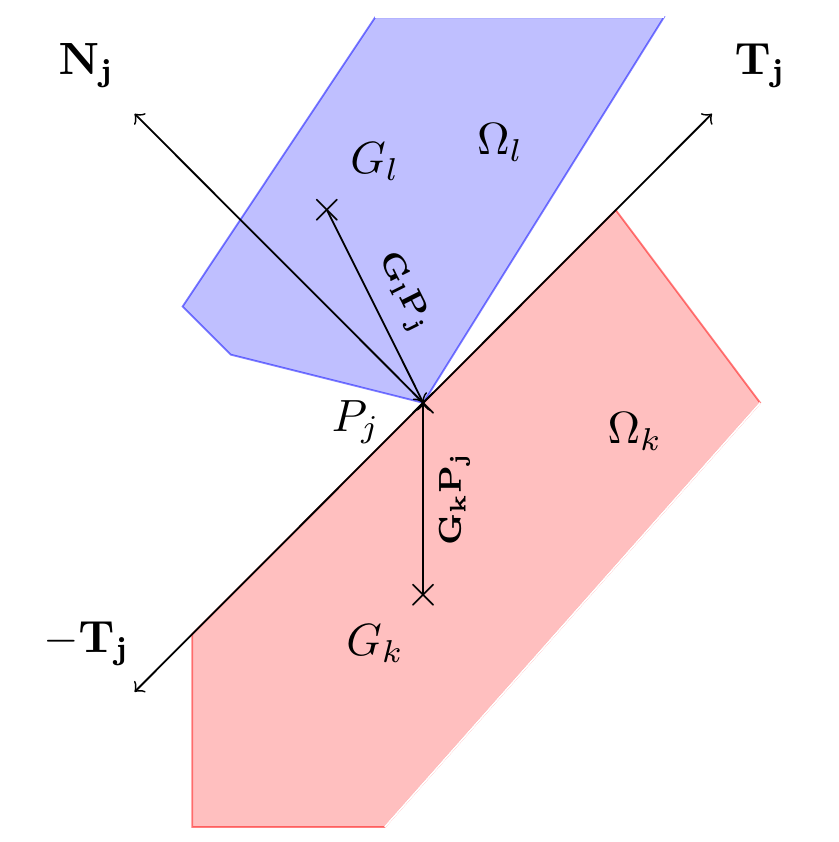
\includegraphics[width=.28\textwidth]{Collision1.png}
%     \caption{Interaction entre deux floes $\Omega_k$ et $\Omega_l$ au point $P_j$ \parencite[p.26]{rabatel2015thesis}.}
%     \label{fig:Collision1}
% \end{figure}

% Soit $P_j$, ($j \in \{1,\ldots,n\}$) un point de contact entre les floes $\Omega_k$ et $\Omega_l$ (voir \cref{fig:Collision1}). Nous notons $\bvec{F}_{kj}(t)$ la force de contact du floe $\Omega_k$ au floe $\Omega_l$ appliquée en $P_j$. Par convention, une matrice de contact $\bmat{M_c}$ est définie telle que son coefficient $c_kj$ vaut :
% \begin{itemize}
%     \item $0\,\,\,\,\,\, $ si le point de contact $P_j$ n’est pas un point de contact du floe $\Omega_k$ ;
%     \item $-1$ si le point de contact $P_j$ est un point de contact entre les floes $\Omega_k$ et $\Omega_l$ avec $k < l$ ;
%     \item $1\,\,\,\,\,\, $ si le point de contact $P_j$ est un point de contact entre les floes $\Omega_k$ et $\Omega_l$ avec $k > l$.
% \end{itemize}
% En notant $E_k$ l’ensemble des points de contact du floe $\Omega_k$ au temps $t$, \parencite[p.26]{rabatel2015thesis} définit la résultante des forces de contact $\bvec{F}^c_k(t)$, au floe $\Omega_k$ comme :
% $$
% \bvec{F}^c_k(t) = \sum_{j \in E_k} c_{jk} \bvec{F}_{kj}(t) \,.
% $$
% En rajoutent ces forces aux forces extérieures lors du bilan des forces à l'\cref{eq:bilan1}, pour un floe $\Omega_k(t)$, on obtient :
% \begin{align} \label{eq:bilan4}
%     \mathcal{M} \frac{\diff W(t)}{\diff t} = \mathcal{H}(t) + \sum_{j \in E_k} \begin{pmatrix}
%         \bvec{F}_{kj}(t) \\ \bvec{G^kP_j} \wedge \bvec{F}_{kj}(t) 
%     \end{pmatrix} \,.
% \end{align}


% \subsubsection{Formulation en problème linéaire de complémentarité}


% Il existe deux principales manières de formuler le problème du contact entre deux solides rigides. L'auteur de \parencite{rabatel2015thesis} opte pour le formalisme vitesse-impulsion, au détriment du formalisme accélération-force. En effet, l’approche en \textbf{vitesse-impulsion} apporte l’avantage de pouvoir exprimer la force de friction de Coulomb directement par rapport à la vitesse. Il n’est pas nécessaire de connaître la nature du contact. Il nous faut donc définir les notions d'impulsion. Sur un intervalle de temps $\delta t^*$, s’il y a un contact entre les floes $\Omega_k$ et $\Omega_l$ au point $P_j$, nous dirons que le floe $\Omega_k$ a subi un choc provenant du floe $\Omega_l$ au point de contact $P_j$ caractérisé par l’impulsion :
% $$
% \bvec{\mathcal{I}}_{kj} = \int_{\delta t^*} c_{kj} \bvec{F}_{kj}(t) \diff t \,.
% $$ 
% \citeauthor{rabatel2015thesis} fait donc apparaître les impulsions dans les équations des moments \cref{eq:bilan1} pour le floe $\Omega_k$ sur l’intervalle temporel $\delta t^*$ :
% $$
% \mathcal{M}_k \int_{\dtstar} \dot{W}_k(t) \diff t = \int_{\dtstar} \mathcal{H}(t) \diff t + \sum_{j \in E_k} \begin{pmatrix}
%     \bvec{\mathcal{I}}_{kj} \\ \bvec{G_kP_j} \wedge \bvec{\mathcal{I}}_{kj} 
% \end{pmatrix} \,.
% $$
% En écrivant $\dtstar = [t^{-}, t^{+}]$, on peut donc introduire les inconnues $\beta$, $\lambda \in (\Rdeux)^m$ pour le problème de contact  
% \begin{align}
%     \mathcal{M} \left( W(t^{+}) - W(t^{-}) \right) = \int_{\dtstar} \mathcal{H}(t) \diff t + \bmat{B}\beta + \bmat{J}\lambda \,,
% \end{align}
% où $\bmat{B}$ et $\bmat{J}$ sont deux matrices de $(\Rtrois)^{n \times m}$telle que
% \begin{align*}
%     \bmat{B} = (d_{kj})_{\substack{1 \leq k \leq n \\ 1 \leq j \leq m}} \,, \quad d_{kj} = \,
%     \begin{cases}
%         0 \in \Rtrois &\text{ si } P_j \text{ n'est pas un point de contact de } \Omega_k \\
%         \begin{pmatrix}
%             c_{kj} \bvec{T}_{j} \\ c_{kj} \bvec{P}_j\bvec{G}_k \wedge \bvec{T}_j 
%         \end{pmatrix} &\text{ si } P_j \text{ est un point de contact de } \Omega_k
%     \end{cases} \,, \\
%     \bmat{J} = (s_{kj})_{\substack{1 \leq k \leq n \\ 1 \leq j \leq m}} \,, \quad s_{kj} = \,
%     \begin{cases}
%         0 \in \Rtrois &\text{ si } P_j \text{ n'est pas un point de contact de } \Omega_k \\
%         \begin{pmatrix}
%             c_{kj} \bvec{N}_{j} \\ c_{kj} \bvec{P}_j\bvec{G}_k \wedge \bvec{N}_j 
%         \end{pmatrix} &\text{ si } P_j \text{ est un point de contact de } \Omega_k
%     \end{cases} \,.
% \end{align*}
% Les matrices $\bmat{B}$ et $\bmat{J}$ sont obtenues par décomposition des forces de contact dans le repère de contact $\mathcal{R}_{\Omega_j} = (P_j, \bvec{T}_j, \bvec{N}_j)$ (voir \cref{fig:Collision1}).

% Comme précédemment mentionné, afin de modéliser la friction dans une collision qui respecte la loi de Coulomb, \parencite{rabatel2015thesis} se base sur les travaux de Stewart et Trinkle \parencite{stewart1996implicit} qui définissent une condition de complémentarité reliant la composante tangentielle $\beta_j$ de l'impulsion appliquée au point $P_j$, la composante normale $\lambda_j$, la vitesse relative tangentielle du point $P_j$ et le coefficient de friction $\mu$. On introduit le vecteur $\tilde{\beta}$ contenant les composantes de l'impulsion tangentielle dans chacune des directions possible de glissement $\bvec{T}_j$ et $-\bvec{T}_j$. Il devient alors possible de formuler le problème de contact (sur tout le système $S$) sans interpénétration par le problème linéaire de complémentarité :
% \begin{align} \label{eq:bilan3}
% \begin{cases} \,\,
%     \begin{pmatrix}
%         0 \\ \bvec{w} \\ \gamma \\ \sigma 
%     \end{pmatrix} =  
%     \begin{pmatrix}
%         \mathcal{M} &  -\bmat{J} & -\bmat{D} & 0 \\
%         \bmat{J}^T & 0 & 0 & 0 \\
%         \bmat{D}^T & 0 & 0 & \bmat{H} \\
%         0 & \mu & -\bmat{H}^T & 0
%     \end{pmatrix} 
%     \begin{pmatrix}
%         W(t^+) \\ \lambda \\ \tilde{\beta} \\ \alpha
%     \end{pmatrix} + 
%     \begin{pmatrix}
%         \int_{\delta t^*} \mathcal{H}(t) \diff t - \mathcal{M} W(t^{-}) \\ 0 \\ 0 \\ 0
%     \end{pmatrix} \\ \quad
%     \begin{pmatrix}
%         \bvec{w} \\ \gamma \\ \sigma
%     \end{pmatrix} \geq 0 \,, \quad
%     \begin{pmatrix}
%         \lambda \\ \tilde{\beta} \\ \alpha
%     \end{pmatrix} \geq 0 \,, \quad
%     \begin{pmatrix}
%         \bvec{w} \\ \gamma \\ \sigma
%     \end{pmatrix} \cdot
%     \begin{pmatrix}
%         \lambda \\ \tilde{\beta} \\ \alpha
%     \end{pmatrix}  
%      = 0 \,,
% \end{cases}
% \end{align}
% avec
% \begin{align*}
%     &\bvec{w} = \bmat{J}^T W(t^+) \,, \quad
%     \bmat{H}^T = (e_{ij})_{\substack{1 \leq i \leq m \\ 1 \leq j \leq 2m}} \,, \quad \tilde{\beta} = (\tilde{\beta}_j)_{1\leq j \leq m} \,, \quad \lambda = (\lambda_j)_{1 \leq j \leq m} \,, \\
%     &\mu \text{ est la matrice diagonale de diagonale} (\mu_1,\dots, \mu_m) \,,\\
%     &e_{ij} = \begin{cases}
%         1 \text{   si } j = 2(i-1) + 1 \text{ ou } j=2(i-1) + 2 \\
%         0 \text{   sinon} 
%     \end{cases} \,,\\
%     &D = (\bvec{B}_1 \vert - \bvec{B}_1 \vert \ldots \vert \bvec{B}_m \vert -\bvec{B}_m) \, \text{   avec } \bvec{B}_j \text{ la colonne } j \text{ de la matrice } \bmat{B} \,.
% \end{align*}
% Le problème consiste alors à trouver les vitesses après contact $W(t^{+})$, à l’aide des composantes inconnues tangentielle et normale des impulsions dans les repères de contact $(\tilde{\beta}\, \gamma)$, elles-mêmes inconnues du système.


% \subsubsection{Consistance énergétique}


% D'après l'auteur de \parencite[p.42]{rabatel2015thesis}, traiter le problème de contact à partir de lois non régulières ne permet pas d’obtenir des solutions satisfaisant à la fois la non-interpénétration, la friction de Coulomb et une consistance énergétique. En se focalisant sur la consistance énergétique, \citeauthor{rabatel2015thesis} a subdivisé le problème en deux : une phase de compression et une phase de décompression suivant la loi de Poisson. La \textbf{phase de compression} modélise la capacité maximale des floes à emmagasiner, par la déformation, une partie ou la totalité de l’énergie cinétique transmise lors du contact. L'impulsion normale $\lambda^c$ calculée durant cette phase (en résolvant le problème de complémentarité (\cref{eq:bilan3})) correspond a un coefficient de restitution $\varepsilon = 0$. Les impulsions obtenues durant cette phase correspondent à celles nécessaire pour éviter la non-interpénétration, et correspondent donc a une énergie cinétique maximale emmagasinée. La \textbf{phase de décompression} correspond à la restitution partielle ou complète de l’énergie cinétique emmagasinée par la déformation des floes. L’impulsion lors de cette phase, notée $\lambda^d$, est déterminée par $\lambda^d = \varepsilon \lambda^c$ (l’hypothèse de Poisson \parencite{glocker1995multiple}). Durant la phase de décompression, \citeauthor{rabatel2015thesis} a donc opté pour la consistance énergétique et la non-interpénétration avec la solution :
% $$
% W^N = (1 + \varepsilon)W^{c} - \varepsilon W(t^{-}) \,,
% $$
% où $W^c$ représente les vitesses des floes après la phase de compression, et $\varepsilon$ le coefficient de restitution pour les contacts considérés inélastiques.

% % \subsubsection{Traitement des conditions aux bords}

% \subsubsection{Le modèle de l'environnement}


% L’environnement est l’ensemble des forces extérieures qui agissent sur les floes hormis les forces de contact qui sont décrites dans la partie précédente. Ces principales forces sont:
% \begin{itemize}
%     \item La force de Coriolis $\bvec{\mathfrak{F}}_c$ donnée pour un floe $\Omega_i(t)$ par:
%     $$
%     \bvec{\mathfrak{F}}_{c,i}(t) = -f\bvec{k} \wedge \dot{\bvec G}_i(t) \,,
%     $$
%     avec $f$ le paramètre de Coriolis et $\bvec{k}$ le vecteur dirigé vers le haut du repère absolu $\mathcal{R}_{abs}$.
%     \item Les forces de trainée associées au vent $\bvec{\tau}_a(t)$ et celle associée à l'océan $\bvec{\tau}_w(t)$: 
%     \begin{align*}
%         \bvec{\tau}_a(t) &= \rho_a C_a \Vert \bvec{U}_a(t) \Vert \bvec{U}_a(t) \,, \\        
%         \bvec{\tau}_w(t,P) &= \rho_w C_w \Vert \bvec{U}_w(t) - \dot{P}(t) \Vert \left(\bvec{U}_w(t) - \dot{P}(t) \right) \,,
%     \end{align*}
%     avec $\rho$ la masse volumique du fluide (l'indice $a$ pour l'air et $w$ pour l'eau) et $C$ un coefficient de traînée sans dimension (voir [HI86]) ; $\bvec{U}_a$, $\bvec{U}_w$, $\dot{P}(t)$ respectivement la vitesse du vent à l'interface glace/fluide, la vitesse du courant oceanique à l'interface glace/fluide, et la vitesse d'un point $P$ du floe. 
% \end{itemize}

% Le modèle de dynamique régulière définit en \cref{eq:bilan1} peut se voire expliciter:
% \begin{align*}
%     \begin{cases}
%             M_i \frac{\diff \dot{\bvec{G}}_i(t)}{\diff{t}} &= M_i \mathfrak{F}_{c,i}(t) + \int_{\Omega_i(t)} \bvec{\tau}_a(t) + \bvec{\tau}_w(t,P) \diff s \,,\\
%             \mathcal{I}_i \frac{\diff \dot{\theta}_i(t)}{\diff t} &= \int_{\Omega_i(t)} \bvec{G}_i\bvec{P} \wedge \left(\bvec{\tau}_a(t) + \bvec{\tau}_w(t,P)\right) \diff s \,.
%     \end{cases}
% \end{align*} 
% L'algorithme décrivant en détail le processus de collision ainsi que la consistance énergétique se trouve à la page 43 du document \parencite{rabatel2015thesis}.


% \subsection{Méthodes numériques et algorithmiques pour la résolution du problème}
 
% \subsubsection{Discrétisation temporelle}

% Pour simuler la dynamique des floes de glace soumis a des forces extérieures et possiblement des collisions, il faut intégrer la dynamique régulière (entre deux collisions), et la dynamique non régulière ; et il existe deux principales méthodes pour la discrétisation en temps dans de tels problèmes. La méthode \textit{\textbf{time-stepping}} (voir \parencite{acary2013projected} pour les schéma de Moreau \parencite{moreau1986dynamique,jean1999non}, et de Schatzman-Paoli \parencite{paoli2002numerical,paoli2002numerical2} par exemple, pour lesquels une convergence a pu être exhibée à partir de la convergence en graphe de Moreau \parencite{moreau1978approximation}) ; comparé aux autres méthodes, la méthode \textit{time-stepping} traite mieux les points d'accumulation \parencite[p.58]{rabatel2015thesis} ; et est plus performante sur des problèmes de multiples contacts. Cependant, \citeauthor{rabatel2015thesis} pour le schéma \textit{\textbf{event-driven}} pour sa précision dans la localisation des collisions et sa facilité de manipulation. En plus, elles permettent d’utiliser des schémas d’intégration existant d’ordre élevé pour des équations différentielles ordinaires. Le seuil de collision choisi est suffisamment grand pour éviter de traiter les collisions une par une. Le schéma utilisé pour intégrer l'équation \cref{eq:bilan1} est un schéma du type Euler explicite, pour sa facilité d’implémentation, sa facilité à prédire la localisation en espace et en temps des futures collisions et enfin, sa capacité à dépasser les problèmes de points d’accumulation. 

% La simulation par la méthode \textit{event-driven} demande la définition d'un pas de temps maximal pour lequel le schéma reste stable. Le pas de temps $\Delta t_max$ sera utilisé si aucune collision n'est détectée entre les instants $t$ et l'instant $t + \Delta t_max$. En se référant au un modèle idéalisé 1D (voir \parencite[p.49]{rabatel2015thesis}), \citeauthor{rabatel2015thesis} distingue deux critères pour la stabilité du schéma numérique au temps $t$ :
% \begin{itemize}
%     \item lorsque la vitesse caractéristique des floes $V_c(t) = N_a \bvec{U}_a(t) + \bvec{U}_w(t)$ est constante sur l'intervalle de simulation $I$, alors pour :  
%     \begin{align} \label{eq:dtmax1}
%         \Delta t \leq \Delta t_{max} = \min{ \left(\frac{\rho}{2 \vert \bvec{U}_a(t) \vert \sqrt{\rho_a C_a \rho_w C_w}} \,, \,\frac{2K_t}{L_t} \right)}
%     \end{align}
%     avec 
%     $$
%     \text{avec } L_t = \rho^{-1} \rho_w C_w \left( N_a^2 \bvec{U}_a^2 + (N_a\bvec{U}_a + 2 \bvec{U}_w)^2 \right) \,, \text{et } K_t = \vert V_c(t) \vert \text{ constant, }
%     $$
%     le schéma est stable c-à-d. $\dot{\bvec{G}} (t + \Delta t) \in [-K_t, K_t] = [-K_{t + \Delta t}, K_{t + \Delta t}]$ ;
%     \item lorsque les variations de $V_c(t)$ entraînent une augmentation de $K_t$ au cours du temps. La propriété de stabilité reste vérifiée car $$\dot{\bvec{G}} (t + \Delta t) \in [-K_t, K_t] \in [-K_{t + \Delta t}, K_{t + \Delta t}] \,;$$
%     \item lorsque les variations de $V_c(t)$ entraînent une diminution stricte de $K_t$ au cours du temps, alors la condition de stabilité dans les deux cas précédents ne peut être vérifiée. \citeauthor{rabatel2015thesis} introduit donc une seconde définition de la stabilité pour traiter ce cas. Il remarque que pour 
%     \begin{align} \label{eq:dtmax2}
%     \Delta t_{max} \leq \begin{cases}
%         \frac{-2x}{\tilde{L}_t^{-}} \text{  si  } x \in  ]-\infty, K_{t+\Delta t}] \\
%         \frac{-2x}{-\tilde{L}_t^{+}} \text{  si  } x \in  ]K_{t+\Delta t}, +\infty]
%     \end{cases}\end{align}
%     avec \begin{align*} \tilde{L}_t^{-} =  \rho^{-1} \rho_w C_w \left[ N_a^2 \bvec{U}_a(t+\Delta t)^2 - (\bvec{U}_w(t + \Delta t) - x)^2 \right] \\ \tilde{L}_t^{+} =  \rho^{-1} \rho_w C_w \left[ N_a^2 \bvec{U}_a(t+\Delta t)^2 + (\bvec{U}_w(t + \Delta t) - x)^2 \right] \,,
%      \end{align*}
%     on a la diminution de la vitesse des floes.
% \end{itemize} 
% En conclusion, pour une vitesse infinitésimale initiale $\dot{G}(0) \in [-K_0, K_0]$, pour tout $t \in I$, et pour tout $\Delta t_{max}$ vérifiant les \cref{eq:dtmax1,eq:dtmax2}, nous avons les vitesses des floes majorées par :
% $$
% \max_{t \in I}{K_t}
% $$
% \citeauthor{rabatel2015thesis} choisi donc de prendre 
% $$
% \Delta t_{max} = \min{ \left( \frac{3}{4} \frac{ -2 \left( \max_{t \in I}{K_t} \right)}{ \max_{t \in I}{\tilde{L}_t^{-}}}, \frac{3}{4} \frac{2 \left( \max_{t \in I}{K_t} \right) }{ \max_{t \in I}{-\tilde{L}_t^{+}}}, \frac{\rho}{2 \left(  \max_{t \in I}{  \vert \bvec{U}_a(t) \vert } \right)  \sqrt{\rho_a C_a \rho_w C_w}} \right)}
% $$
% pour s'assurer que le modèle idéalisé vérifie les critères de stabilité définis. 
% Notons que le procédé global d’intégration de la dynamique pour le modèle se situe à la figure 2.2 du document \parencite[p.60]{rabatel2015thesis}, le schéma est repris à la \cref{fig:Algo1}.

% \begin{figure}[!ht]
%     \centering
%     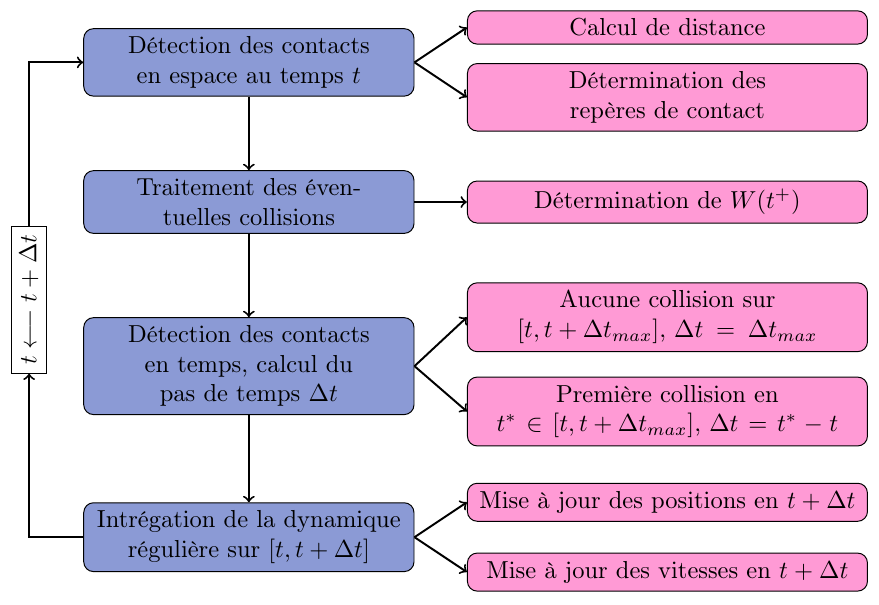
\includegraphics[width=.62\textwidth]{Algo1.png}
%     \caption{Procédé global d’intégration de la dynamique pour notre modèle \parencite[p.60]{rabatel2015thesis}.}
%     \label{fig:Algo1}
% \end{figure}


% \subsubsection{Détection des collisions en espace}

% Des deux méthodes principales utilisées dans la littérature pour la détection des voisins, \citeauthor{rabatel2015thesis} a choisi la méthode de \textbf{hiérarchie de volumes englobants} pour sa facilité de mise en place et pour son efficacité même avec de grands ratios de tailles. L'alternative était la méthode de \textbf{partitionnement de l'espace} qui elle, souffre de plusieurs défauts non surmontables pour le modèle développé. Les méthodes de volumes englobants consistent à englober le contour de l’objet par des volumes à des échelles de plus en plus fines pour améliorer la détection.

% \subsubsection{Détection des contacts en temps}

% Il s'agit ici de trouver le pas de temps optimal c’est-à-dire un pas de temps $\Delta t$ pour lequel la configuration des floes ne contenant pas d’interpénétrations sur l’intervalle de temps $[t, t + \Delta t]$ et, pour tout $\varepsilon > 0$, contient au moins une interpénétration sur l’intervalle de temps $[t + \Delta t, t + \Delta t + \varepsilon]$ \parencite[p.87]{rabatel2015thesis}.
% Lorsque le critère de collision n’est pas vérifié, \citeauthor{rabatel2015thesis} montre qu'il suffit de prendre 
% $$
% \Delta t_{i,j} = -\frac{-\delta_{i,j(t)} - tol_3}{\bvec{A}_{ij}(t) \cdot \left( \dot{G}_i(t) - \dot{G}_j(t) \right)} \,,
% $$
% avec 
% $$
% \bvec{A}_{i,j}(t) = \frac{C_{0,i}(t) - C_{0,i}(t)}{d\left(C_{0,i}(t), C_{0,i}(t) \right)} \,, \text{ et  } \quad tol_3 = \frac{\xi}{20} \,.
% $$
% Lorsque le critère de collision est vérifié, il faut plutôt prendre 
% $$
% \Delta t_{i,j} = \frac{\min{\left( \eta_i, \eta_j \right) - tol_3}}{\Gamma(t)} \,,
% $$
% avec 
% $$
% \Gamma(t) = \max{\left( \Vert \dot{Q}_i^{i,j}(t) \Vert \,, \, \Vert \dot{Q}_j^{j,i}(t) \Vert  \right)} \,,
% $$
% où $\dot{Q}_i^{i,j}$ représente la distance parcourue par un point de $\Omega_i (t)$ relativement à $\Omega_j (t)$.

% Une fois ce $\Delta t_{i,j}$ assurant la non-interpénétration trouvé, on peut donc choisir 
% $$
% \Delta t = \min{\left( \Delta t_{max} \,, \min_{ \substack{ (i,j) \in \left\{ 1,\ldots,n \right\}^2 \\ i \neq j}}{\Delta t_{i,j}} \right)} \,.
% $$
% Le lecteur est renvoyé au document \parencite[p.91]{rabatel2015thesis} pour plus de détails sur la détection des contacts en temps.

% \subsubsection{Construction des repères de contacts}

% La construction d'un repère de contact n'est effectuée que lorsque le contact entre deux floes $\Omega_k$ et $\Omega_l$ est \textbf{linéique} \parencite[p.79]{rabatel2015thesis}, ou \textbf{ponctuel} et le vecteur porté par les points en contacts appartient au cône normal de $P$. La normale $\bvec{N}$ est alors déterminée comme le vecteur unité dirigé par $\bvec{PQ}$. Si $Q$ n’est pas unique, on se retrouve dans la situation où il peut exister plusieurs repères de contact pour un point de contact. Dans les autres cas, le repère de contact associé au point $P$ n’est pas construit et $P$ n’est pas considéré dans le traitement des contacts \parencite[p.80]{rabatel2015thesis}. L'algorithme de détection des points de contacts afin de construire les repère de contact est explicité dans le document \parencite[p.76]{rabatel2015thesis}. 


% \subsubsection{Simulation des événements collisions}

% Une fois les voisins détectés et les repères de contact construits, on peut passer à la prochaine étape qui consiste en la simulation des évènements de collisions. Ici, plusieurs choix s'offrent à nous : les méthodes dites de \textbf{régularisations}, les méthodes dites \textbf{itératives}, et les méthodes dites \textbf{de pivots} \parencite[p.82]{rabatel2015thesis}. La première catégorie est adaptée aux modèles régularisants, ce qui n'est le cas de notre modèle. La deuxième par contre a extensivement été utilisée dans la littérature ; on peut citer Moreau \parencite{moreau1988unilateral,moreau1999numerical,jean1999non}, Aitken \parencite{aitken1950iv}. Malheureusement, dès que la matrice $A$ du problème de complémentarité à résoudre n'est plus symétrique, ce deuxième groupe de techniques ne s'avère pas efficace. \citeauthor{rabatel2015thesis} choisi donc l'algorithme de Lemke pour lequel il existe des preuves de convergence lorsque la matrice $A$ est co-positive. Bien qu'il soit performant, il faut néanmoins noter que l’algorithme de Lemke étant une technique globale, c’est-à-dire traitant les contacts simultanément, il ne garantit pas une bonne propagation du contact \parencite[p.82]{rabatel2015thesis}.

% \subsubsection{Optimisations}

% La première optimisation apporté est celle sur les distances de collision : deux floes sont en contact si la distance entre eux n'est pas nulle, mais supérieure à un seul appelée \textbf{distance de collision}.

% La deuxième concerne la condition de non-interpénétration \parencite[p.85]{rabatel2015thesis}. En cas de congestion, il est difficile que les floes décollent après contact. En exigeant que $\bmat{J}^T W(t^+) > 0$ après collision, on risque ne pas avoir de solution pour le problème linéaire de complémentarité associé. \citeauthor{rabatel2015thesis} relaxe donc la condition de Signorini en définissant un réel $c$, et l'ensemble des vitesses admissibles devient donc :
% $$
% V_c = \left\{ w \in \mathbb{R}^{3n} \, | \, \bmat{J}^T w \geq c \right\} \,.
% $$
% Une troisième optimisation concernant la définition de la \textbf{notion d'erreur} et de \textbf{tolérance} a été implémentée. La quatrième consiste en la résolution d'un LCP en trois tentatives (avec trois algorithmes de Lemke différents) même si cela augmente les coups de calculs \parencite[p.86]{rabatel2015thesis}. Si cette optimisation ne s'avère pas suffisance, une dernière optimisation consiste en la modification aléatoire de certains coefficients de la matrice $A$, la permutation des lignes afin d'éviter des zéros sur la diagonale, ou encore l'utilisation de la notion de \textbf{contact actif}.


% \subsection{Validations et exploitations du modèle}

% Les résultats ont été validés à travers plusieurs expériences. Nous citons des exemples classique tels que la \textbf{boîte glissante}, le \textbf{berceau de Newton}, le \textbf{canon de Newton}, la \textbf{balle rebondissante}, etc. Le modèle a ensuite été validé sur des scénarios simples de dérive libre soumise à des courants océanique et atmosphérique et des scénarios simples de collision. En effet, il a été vérifié que le comportement d’un objet simulé est cohérent avec le comportement théorique et avec les observations. Les principes physiques suivants ont ainsi pu être testé par \citeauthor{rabatel2015thesis} :
% \begin{itemize}
%     \item la conservation de la symétrie d’une configuration ;
%     \item la satisfaction du modèle de Coulomb ;
%     \item le traitement d’un point d’accumulation ;
%     \item la cohérence temporelle ou la propagation des ondes de choc ;
%     \item la conservation de l’énergie cinétique.
% \end{itemize} 
% Des telles exploitations telles que la dérive dans un canal étroit, pour des floes en bassins a été étudié (voir \cref{fig:Derive,fig:DeriveSol}). Aussi, la dérive soumise à un vent et un courant variable avec des vitesses du vent provenant de \textbf{ERAinterim}, à partir du modèle glace de mer et océan \textbf{TOPAZ} a été étudiée.

% \begin{figure}[!ht]
%     \centering
%     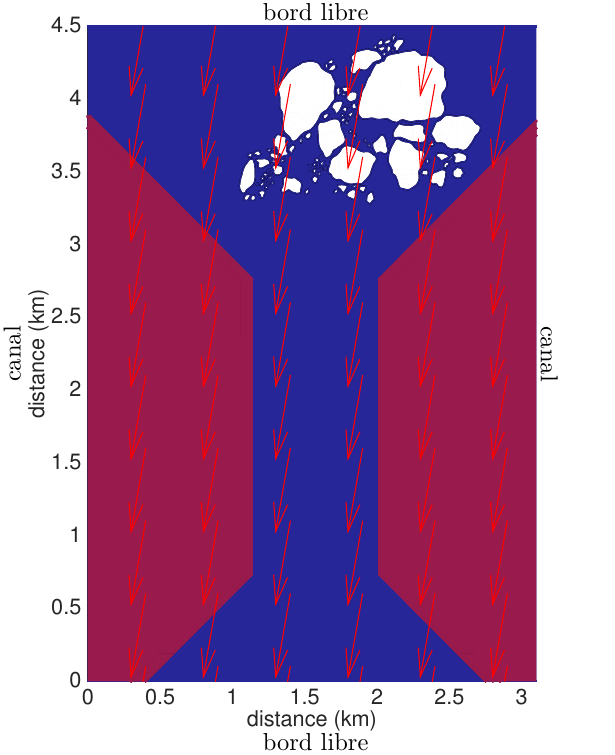
\includegraphics[width=.28\textwidth]{Derive.png}
%     \caption{Configuration à l’instant initial pour le scénario de dérive dans un canal étroit \parencite[p.124]{rabatel2015thesis}.}
%     \label{fig:Derive}
% \end{figure}

% \begin{figure}[!ht]
%     \centering
%     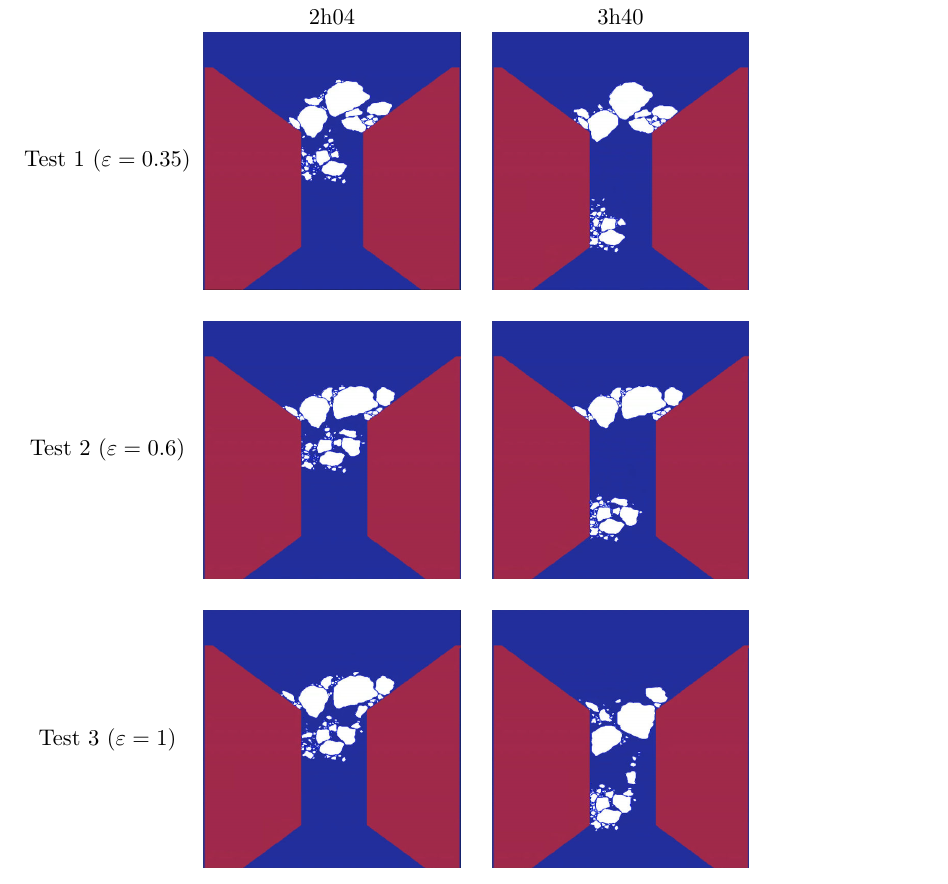
\includegraphics[width=.68\textwidth]{DeriveSol.png}
%     \caption{Quelques résultats obtenus à deux heures différentes de la configuration des floes pour différentes valeurs du coefficient de restitution $\varepsilon$ \parencite[p.126]{rabatel2015thesis}.}
%     \label{fig:DeriveSol}
% \end{figure}

% \subsection{Discussion}
% Bien que les travaux de \citeauthor{rabatel2015thesis} ont été testés et validés sur plusieurs configurations différentes, il reste néanmoins des points qui ne sont pas traités, et qui ont très clairement été soulignés dans la thèse \parencite{rabatel2015thesis} :
% \begin{enumerate}
%     \item Le modèle ne gère pas la rhéologie\footnote{La rhéologie est l'étude de la déformation et de l'écoulement de la matière sous l'effet d'une contrainte appliquée.} de la glace : les floes sont des solides purement rigides (ils ne se déforment pas) et la dissipation d’énergie cinétique durant la collision est décrite en utilisant un coefficient purement empirique collision.  
%     \item La loi de contact utilisée pour le glissement (voir \parencite{stewart1996implicit}), bien que très riche, ne prends pas en compte toutes les vitesses possibles de déplacement. La construction d’une loi qui donnerait accès à la région entière, demanderait de prendre en compte un grand nombre de phénomènes intrinsèques aux contacts. Leur compréhension et leur rôle à chacun est difficile à déterminer. 
%     \item Les coefficients de friction et de restitution utilisées sont limitants. En réalité, il n’est pas possible de prendre en compte ou d'interpréter mathématiquement certains effets lors du contact ; par exemple, avec la dispersion de l'énergie (voir \parencite{nguyen2014multiple}). Cette dispersion est la conséquence de certains effets vibratoires à travers une chaîne de contact. Seuls les effets de dissipation dus aux phénomènes locaux comme l’endommagement, la viscosité ou la plasticité sont pris en compte à travers l’utilisation des coefficients de restitution et de friction.
%     \item Les vitesses obtenues après la phase de décompression afin d'assurer la dissipation de l'énergie cinétique possèdent une faiblesse : elles ne sont solutions que sous certaines conditions, comme le fait que les chocs soient frontaux et qu’il n’y ait pas d’apport des forces extérieures autres que les forces de contact durant la collision \parencite[p.41]{rabatel2015thesis}.
% \end{enumerate}

% %----------------------------------------------------------------------------------------



%----------------------------------------------------------------------------------------

\section{Résumé de thèse de D. Balasoiu}

Les travaux de D. Balasoiu concernent la modélisation et la simulation du comportement mécanique de floes de glace \parencite{balasoiu2020thesis}. Il s'agit d'une amélioration des travaux de M. Rabatel, S. Labbé, et J. Weiss \parencite{rabatel2015thesis,rabatel2015dynamics} prenant en compte la fracture des floes. Précisément, ce travail se focalise sur l’initiation de la fracture, ainsi que la prédiction du chemin que la fracture emprunte. Jusqu’à présent, les floes étaient considérés comme des corps rigides ; dans sa thèse, \citeauthor{balasoiu2020thesis} les considère comme des corps élastiques. Son travail est divisé en deux parties. Il commence par proposer un modèle efficace pour la fracture fragile d’un floe de glace, lorsque celui-ci est soumis à un déplacement de son bord (i.e. à une condition au bord de type Dirichlet). Puis, dans un second temps, il cherche à obtenir l’expression du déplacement au bord d’un floe qui percute un autre floe ou une structure solide.

\subsection{Théorie de la fracture : état de l’art} 
 
La théorie de fracture la plus répandue de nos jours est due à A.A. Griffith. Dans ses travaux[Gri21], in invalide les résultats que C. Inglis [Ing13] qui ne tenaient pas en compte la taille de la fracture ; il présente donc la croissance d'une faille comme une compétition d'énergie entre l'énergie élastique\footnote{Énergie relâchée lorsqu’un défaut subit un accroissement. Cette énergie diminue durant la fracture.} et l'énergie de surface\footnote{Énergie nécessaire à la création des deux nouvelles surfaces – les bords de la fissure. Cette énergie augmente avec l'accroissement de la fracture.}. 

Le critère de Griffith est un critère thermodynamique qui stipule que la fracture progresse si et seulement si cela permet au matériau d’atteindre un état de moindre énergie. En effet, sur un matériau élastique $\Omega$ dont la frontière est subdivisée en deux zones $\partial \Omega_D$, et $\partial \Omega_N$, on pose \parencite[p.31]{balasoiu2020thesis} :
\begin{align*}
    E_{el} &= \int_{\Omega} W (x, e(u)) \diff x     \\
    \mathcal{P}(t,\sigma(t)) &= \int_{\Omega \backslash \sigma(t) } W (x, \nabla\varphi (t, \sigma(t))) \diff x - \mathcal{F}(t,\sigma(t)) \\
    \mathcal{F}(t,\sigma(t)) &= \int_{\Omega} f_v (x)\cdot \varphi \diff x + \int_{\partial\Omega_N} f_s (x) \cdot \varphi \diff x
\end{align*}
où 
\begin{itemize}
    \item $E_{el}$ est l'énergie élastique du matériau sans faille.
    \item $\sigma(t)$ représente la fracture au temps $t$, supposée à l'équilibre.
    \item $\mathcal{P}$ l’énergie potentielle du matériau qui possède une fracture de taille $\sigma(t)$ au temps $t$.
    \item $e(u)$ est le tenseur de Green-St Venant, qui représente la déformation locale du matériau.
    \item $\varphi = \identity + u$ représente le déplacement du matériau supposé suffisamment régulier.
    \item $W$ est la densité d’énergie du matériau élastique, supposé hyper-élastique.
    \item $f_s$ est la contrainte surfacique appliquée sur le bord $\partial \Omega_N$.
    \item $f_v$ est le champ de force volumique appliquée sur $\Omega$.
\end{itemize}
D'après le critère de Griffith \parencite[p.32]{balasoiu2020thesis}, la fonction $\sigma(t)$ doit vérifier :
\begin{enumerate}
    \item $\dfrac{\diff \sigma(t)}{\diff t} \geq 0$ ;
    \item $-\dfrac{\diff \mathcal{P}}{\diff \sigma} (t,\sigma(t)) \leq k$ ;
    \item $\dfrac{\diff \sigma(t)}{\diff t} > 0 \Rightarrow -\dfrac{\diff \mathcal{P}}{\diff \sigma} (t,\sigma(t)) = k$.
\end{enumerate}

\begin{figure}[!ht]
    \centering
    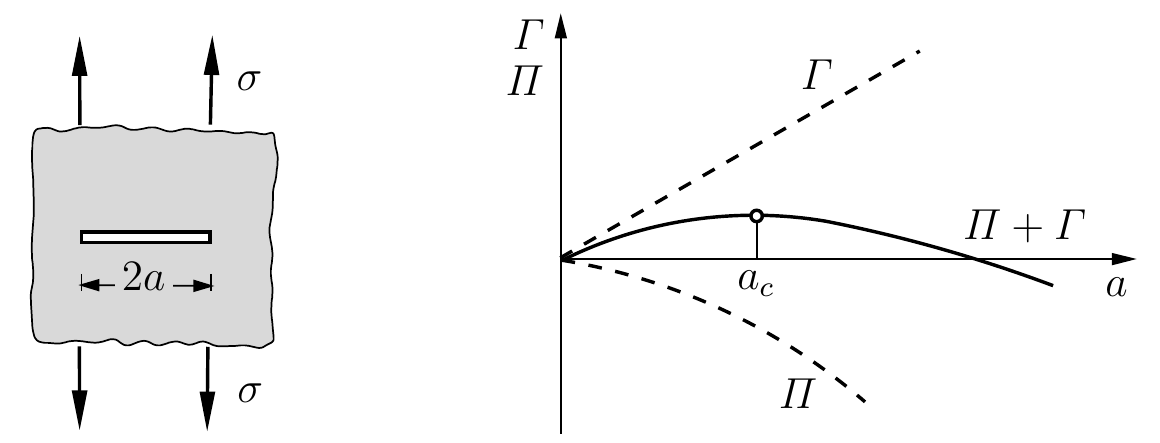
\includegraphics[width=.8\textwidth]{Griffith.png}
    \caption{Illustration du critère de Griffith \parencite{gross2017fracture}. ($\Pi$ et $\Gamma$ représentent les énergies potentielles et de fracture respectivement. \textit{Cette figure est à refaire manuellement !})}
    \label{fig:Griffith}
\end{figure}
Une illustration de ce critère peut être observée à la \cref{fig:Griffith}. Comme mentionné plus haut, ce modèle souffre de problèmes de nucléation et de prédiction de la fracture. Pour contourner le problème de nucléation, les mécaniciens considèrent que tout matériau possède des microfissures, et ce sont ces dernières qui sont à l'origine des fissures observables à l'\oe{}il. Quant au problème du chemin emprunté par la fracture, A. Chambolle, G. Francfort et J.-J. Marigo [CFM09] montrent que les critères d'Irwin [Irw57] sont invalides car, ils impliquent que, dans un matériau homogène et isotrope, le chemin de la fracture ne peut être courbé.

Le modèle proposé par Francfort et Marigo [FM98], suit un résultat théorique dû à De Giorgi, M. Carriero et A. Leaci [DCL89], qui prouvent le théorème d’existence d'un minimum pour la fonctionnelle de Mumford-Shah qui intervient dans la détection des contours d’une image. Présentons les données géométriques du problème \parencite[p.35]{balasoiu2020thesis}. Soit $\Omega \subset \mathbb{R}^N$ un ouvert connexe, dont la frontière $\partial \Omega$ est suffisamment lisse. On partitionne sa frontière :
$$
\partial \Omega = \partial \Omega_D \cup  \partial \Omega_N \,,
$$
où $\partial \Omega_D$ et $\partial \Omega_N$ sont les bords où l’on applique respectivement des conditions de Dirichlet et de Neumann. Sur la partie Dirichlet, on applique un déplacement du bord noté $U_D$, tandis que l’on laisse libre la partie de Neumann. On suppose également que le matériau est soumis à un champ de force volumique $f_v$. On suppose que $\Omega$ est un matériau hyper-élastique, dont la densité d’énergie est notée $W$. Ainsi, lorsque le matériau $\Omega$ subit (sans fracture) une déformation $\varphi = u + \identity$ suffisamment lisse, son énergie élastique vaut :
$$
\eel(u) = \int_{\Omega} W(x,e(u)) \diff x \,,
$$
où l’on a noté $u$ le champ de déplacement du matériau, et $e(u)$ son gradient symétrisé. On notera l’énergie élastique du matériau qui présente une fracture $\sigma$ :
$$
\eel(u,\sigma) = \inf_{u\in V_{U_D, \sigma}}{\int_{\Omega \backslash \sigma} W(x,e(u)) \diff x} \,,
$$
où l’on a défini l’espace fonctionnel $V_{U_D,\sigma}$ ,σ par :
$$
V_{U_D,\sigma} = \left\{ u \in H^1(\Omega \backslash \sigma, \mathbb{R}^N) \, \rvert \, u = U_D \text{ sur } \partial \Omega_D \right\} \,.
$$
Francfort et Marigo proposent l’énergie de fracture suivante sur $\partial \Omega_D$ :
$$
\efrac(\sigma) = \int_{\sigma} k(x) \diff \mathcal{H}^{N-1} \,,
$$
où le champ scalaire $k(x)$ traduit la rigidité du matériau, et est supposée strictement positive sur tout le matériau ; $\mathcal{H}^{N-1}$ représente la mesure de Haussdorf de dimension $N-1$, qui peut être comprise comme la longueur du contour pour $N=2$.

Ainsi, l’énergie totale du matériau vaut :
\begin{align*}
\etot(u,\sigma) &= \eel(u,\sigma) + \efrac(\sigma) \\
&= \int_{\Omega \backslash \sigma} W(x,e(u)) \diff x + \int_{\sigma} k(x) \diff \mathcal{H}^{N-1} \,,
\end{align*}
où $\sigma$ est une union dénombrable d'ensembles rectifiables. Ainsi donc, une solution du problème de fracture est un minimum de la fonctionnelle $\etot$. Signalons que \citeauthor{balasoiu2020thesis} montre, dans le cas d'un mouvement antiplan\footnote{Un mouvement \textbf{antiplan} est mouvement pour lequel le champ de déplacement $u$ est porté par un vecteur constant.}, que le modèle est quasiment identique au modèle de De Giorgi, M. Carriero et A. Leaci, pour lequel un théorème d'existence a pu être exhibé.

La méthode numérique employée est la méthode à champ de phases. Elle repose sur la notion de $\Gamma$-convergence, en particulier sur le résultat de \textbf{convergence des minimums}. On remplace l'inconnue $\sigma$ par une suite de fonctions lisses $v_\varepsilon$ [AT90]. Par exemple, dans le cas du traitement d'image, pour la fonctionnelle de Mumford-Shah dont se sont inspiré Bourdin, Francfort et Marigo, on constate d'après Ambrosio et Tortorelli [AT90] que la suite de fonctionnelle
$$
G_{\varepsilon}() = \int_{\Omega} \left( \vert u-g \vert^2 + (v^2 + \eta_{\varepsilon}) \vert \nabla u \vert^2 + \varepsilon \vert \nabla v \vert^2 + \frac{(v-1)^2}{4\varepsilon} \right) \diff x \,,
$$
$\Gamma$-converge vers la fonctionnelle limite 
$$
G_f = \int_{\Omega} \vert u-g \vert^2 + \vert \nabla u \vert^2 \diff x + \mathcal{H}^{N-1}(S_u) \,,
$$
où $g:\Omega \mapsto [0,1]$ est la fonction de contraste de l’image, et $\mathcal{H}^{N-1}(S_u)$ est la restriction de la mesure de Hausdorff à l’ensemble des sauts de $u$, noté $S_u$, qui est un ensemble mesurable et composé d’une union dénombrable d’ensembles rectifiables \parencite[pp.33-35]{balasoiu2020thesis}.

Plusieurs études numériques reposant sur ce résultat de $\Gamma$-convergence sont disponibles dans la littérature. On cite par exemple ici les résultats obtenus dans [Nag+19] à la \cref{fig:PhaseField}.

\begin{figure}[!ht]
    \centering
    \begin{subfigure}[b]{0.9\textwidth}
        \centering
        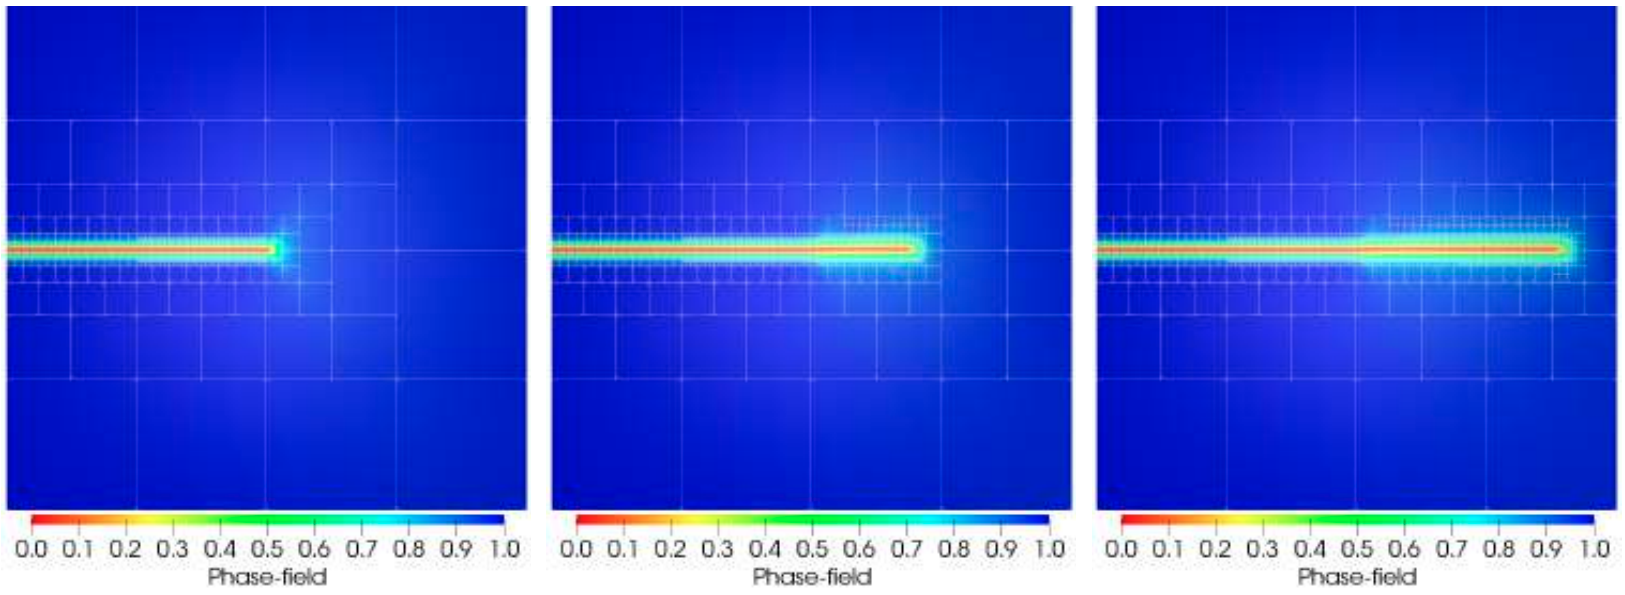
\includegraphics[width=\textwidth]{PhaseField1.png} 
        \caption{Croissance d’une fracture}
        \label{fig:PhaseField1}
    \end{subfigure}
    \begin{subfigure}[b]{0.9\textwidth}
        \centering
        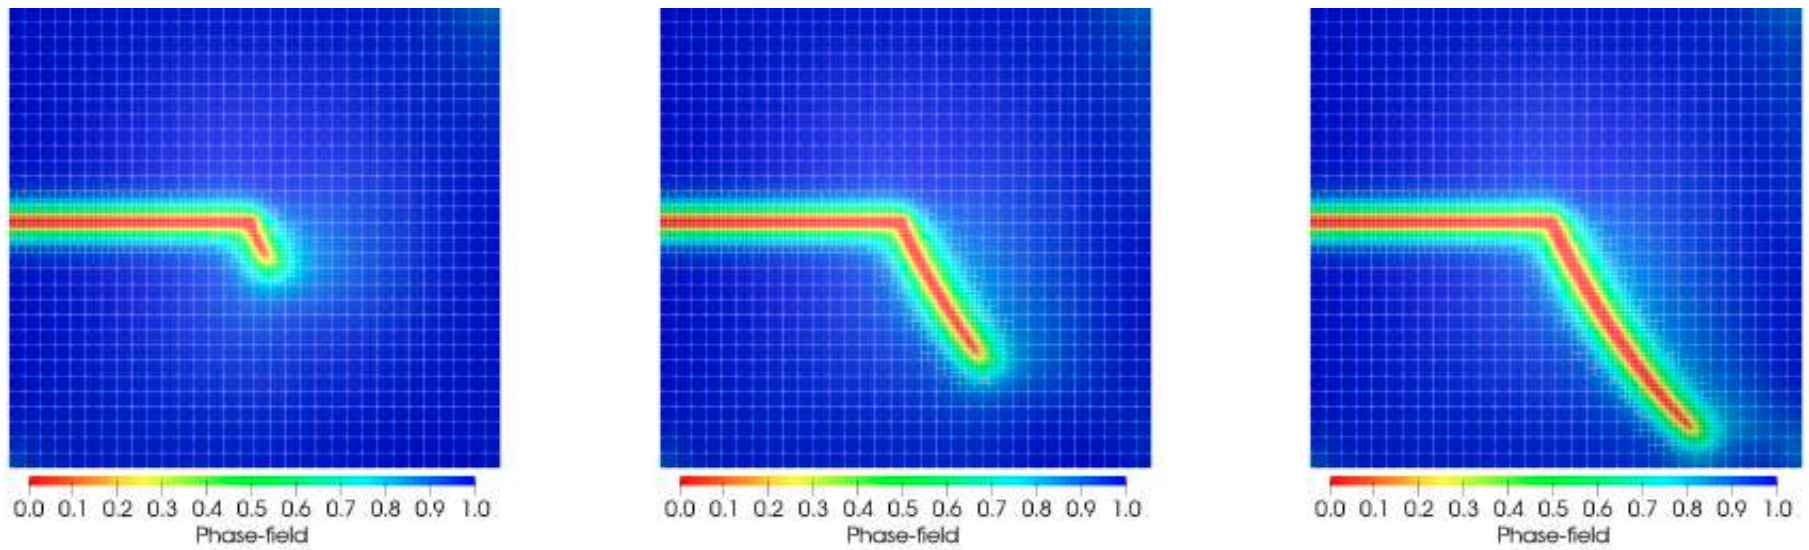
\includegraphics[width=\textwidth]{PhaseField2.png} 
        \caption{Bifurcation d’une fracture}
        \label{fig:PhaseField2}
    \end{subfigure}
    \begin{subfigure}[b]{0.9\textwidth}
        \centering
        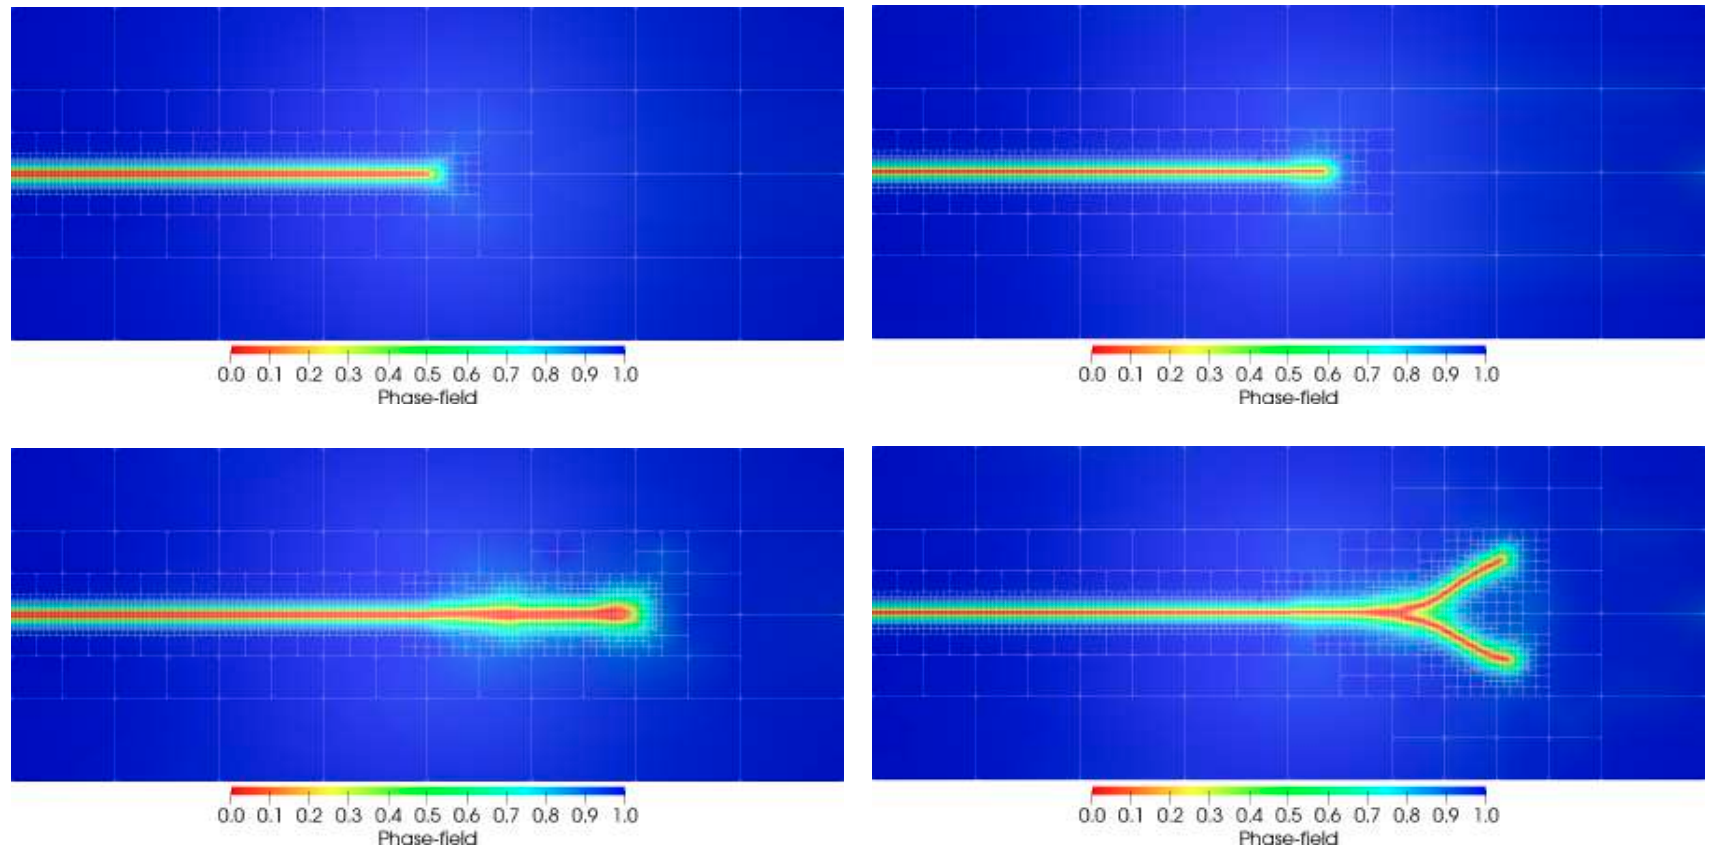
\includegraphics[width=\textwidth]{PhaseField3.png} 
        \caption{Branchement d’une fracture}
        \label{fig:PhaseField3}
    \end{subfigure}
       \caption{Trois résultats numériques obtenus dans [Nag+19] à l'aide d'une discrétisation éléments finis (hp-FEM) et volumes finis en ne remaillant le domaine que lorsque c'est nécessaire.}
       \label{fig:PhaseField}
\end{figure}


\subsection{Un modèle de fracture variationnel et efficace} 

Le modèle présenté dans la section précédente n'est pas adapté à notre étude. \citeauthor{balasoiu2020thesis} a donc développé un modèle qui ne nécessite pas de fonctionnelle lissée, comme l'on fait plusieurs modèles de glaciologie (voir [LLL15]), en supposant que les fractures sont des segments. Un résultat d'existence (dans les cas où le floe n'est pas encore fracturé) est prouvé à l'aide de la convergence de Mosco. De plus, \citeauthor{balasoiu2020thesis} introduit un problème d’évolution quasi-statique en appliquant progressivement la condition de Dirichlet sur une partie du bord du floe. Les fractures obtenues par ce problème d’évolution sont ainsi des lignes brisées. Le résultat d'existence n'a pas été prouvé pour ce cas. Concernant le côté numérique, une méthode \textit{meshless}\footnote{Car l’ensemble discrétisé des fractures admissibles ne dépend pas du maillage utilisé.} est proposée.

Les modifications apportées pour traiter le modèle statique (dans $\Rdeux$) sont décrites ci-bas. Lorsqu'on fixe la fracture $\sigma$, l'énergie élastique prend la forme :
\begin{align*}
\eel (\cdot,\sigma): \, A_{\sigma} &\rightarrow \mathbb{R} \\
u &\mapsto \int_{\Omega \backslash \sigma} Ae(u) : e(u) \diff x \,,
\end{align*}
où $A$ représente le tenseur de Lamé du matériau, i.e.
$$
    \forall e \in M_2{\mathbb{R}}, \quad Ae = \lambda \text{ tr }(e)I_2 + 2\mu e \,,
$$ 
où $\lambda$ et $\mu$ sont les coefficients de Lamé du matériau ; et l'ensemble des déplacements admissibles $A_{\sigma}$ est :
$$
A_{\sigma} = \left\{  u \in H^1(\Omega \backslash \sigma \, \mathbb{R}^2) \, \rvert \, u=U_D \text{ sur } \partial \Omega_D \backslash \sigma \text{ et } (u^+ - u^{-}) \cdot \nu \text{ sur } \sigma \right\} \,,
$$
avec $u^{+}$ et $u^{−}$ les restrictions de $u$ aux régions $\Omega^{+}$ et $\Omega^{-}$ respectivement (obtenues par extension de la fracture $\sigma$ de façon à ce qu'elle soit traversante \parencite[p.50]{balasoiu2020thesis}). $\nu$ (normale à la fracture orientée du bord vers le centre de $\Omega$) et $−\nu$. On note la présence d'une condition de type Signorini :
$$
(u^+ - u^{-}) \cdot \nu \geq 0 \text{  sur  } \sigma
$$
L'énergie totale s'écrit
\begin{align*}
\etot : \,\bigcup_{\sigma \in \Sigma } A_{\sigma} \times \left\{ \sigma \right\} &\rightarrow \mathbb{R} \\
 u &\mapsto \int_{\Omega \backslash \sigma} Ae(u) : e(u) \diff x + k\mathcal{H}^1(\sigma)\,,
\end{align*}
où $\Sigma$ représenté l'ensemble les segments orientés partant de la frontière donnée par 
$$
\Sigma = \left\{ [a,b] \in \mathbb{R}^2 \, \lvert \, a \in \partial\Omega, b\in \overline{\Omega}, ]a,b[ \in \Omega\right\} \,.
$$
Une solution de notre modèle de fracture fragile est un couple $(u, \sigma)$ qui vérifie
$$
\etot(u,\sigma) = \min_{\sigma \in \Sigma}{\min_{u\in A_{\sigma}}{\etot(u,\sigma)}} \,.
$$
Ensuite, \citeauthor{balasoiu2020thesis} remarque que la solution n'est pas unique. Il définit donc un problème de d'évolution quasi-statique à la manière de [FM98], en considérant un problème de chargement monotone : 
$$
U_D(t) = tU_D \,.
$$
On note $\overline{\Sigma}$ l’ensemble des lignes brisées de $\Omega$, sans point d’auto-intersection et qui partent de la frontière. On note également $\text{end}(\sigma)$ la fin d’une ligne brisée $\sigma \in  \overline{\Sigma}$.
On définit maintenant \parencite[p.48]{balasoiu2020thesis}, pour toute ligne brisée $\sigma \in  \overline{\Sigma}$ l’ensemble des fractures admissibles partant de $\sigma$ :
$$
\Sigma_{\emptyset} = \Sigma \,, \quad \Sigma_{\sigma} = \left\{ \sigma \cup [a,b] \in \mathbb{R}^2 \, \lvert \, a = \text{end}(\sigma), b\in \overline{\Omega}, ]a,b[ \in \Omega\backslash \sigma \right\} \,.
$$
On définit également l'ensemble des déplacements admissibles associées :
$$
A_{t,\sigma} = \left\{  u \in H^1(\Omega \backslash \sigma \, \mathbb{R}^2) \, \rvert \, u=tU_D \text{ sur } \partial \Omega_D \backslash \sigma \text{ et } (u^+ - u^{-}) \cdot \nu \text{ sur } \sigma \right\} \,,
$$
pour tout $t \in [0,1]$ et pour toute ligne brisée $\sigma$. De ces définitions, on peut en exhiber un problème d'évolution discret, et un problème d'évolution continue en faisant tendre $t$ vers $0$. Le problème d’évolution continue admet des solutions, comme limite de solutions des problèmes d’évolutions discrets [MT02 ; Cha03].

Lorsque la fracture est fixée, \citeauthor{balasoiu2020thesis} prouve l’existence de solutions à notre problème de minimisation, en utilisant la théorie des inégalités variationnelles, l'inégalité de Korn [Cia94], le théorème de Lions-Stampacchia [LS67]. Pour le cas statique, il montre que le problème statique a des solutions lorsque l’ouvert n’est pas encore fracturé, ceci en se servant principalement de la convergence de Mosco. Pour le modèle quasi-statique, un résultat d'existence n'a pas été trouvé, et une conjecture pour une ligne brisée qui possède un point d'auto-intersection a été proposée.



\subsection{Étude asymptotique d’un réseau de ressorts régulier} 

Dans ce chapitre, \citeauthor{balasoiu2020halthesis} souhaite approcher l’énergie élastique d’un matériau continu par l’énergie élastique d’un réseau de ressorts, dans un cadre statique, lorsque celui-ci est soumis à un déplacement de son bord. Autrement dit, nous ne nous intéressons pas au mouvement des particules, nous n’étudions que l’état d’équilibre du réseau de ressorts.

Commencions par quelques définitions pour le maillage sur un floe. Pour définir un réseau de ressort $\tau$, on définit l'ensemble de ses points $\tau_0$ disposées en forme de grille. 
$$
\tau_0 = \Omega \cap \mathbb{Z}^2
$$
De façon similaire, l'ensemble des arrêtes se nomme $\tau_1$, et l'ensemble des cellules $\tau_2$. Le réseau $\tau$ est obtenu à partir de $\tau_0$ en traçant les côtés de chaque carré ; à la frontière, on trace les diagonales des carrés incomplets. On note $W (\tau, \Rdeux)$ l’ensemble des fonctions de $\tau_0$ dans $\Rdeux$. On définit également deux triangulations de $\omega$ à partir de $τ$, en prenant respectivement les diagonales des carrés dans les directions $e_x + e_y$ et $e_x − e_y$. On note ces triangulations $\tilde{\tau}$ et $\hat{\tau}$ respectivement. 

Afin d'éviter les déformations qui envoient deux points voisins sur le même point, on définit avec l'ensemble des déplacements admissibles 
$$
\wadm(\tau, \Rdeux) =   \left\{ u\in W(\tau, \Rdeux) \mid \forall w \in \tau_2, \forall q_1, q_2 \in \tau_0 \cap \overline{\omega}, q_1 \neq q_2, \quad q_1 + u(q_1) \neq q_2 + u(q_2)  \right\} \,,
$$
Sur chaque arête $\nu ∈ \tau_1$, on place un ressort de longueur à vide $l_{\nu} = \vert \nu \vert$, et de raideur $k_{\nu}$ (voir \cref{fig:Ressort1}). Si $\varphi \in W (\tau, \Rdeux)$ est une déformation du réseau de ressorts, et $u = \varphi − \identity$ est le déplacement associé, l’énergie élastique de traction de l’assemblage
\begin{align*}
    R_{\tau}(u) &= R_{\tau}(\varphi - \text{Id}) \\
    &= \sum_{\nu \in \tau_1} \frac{k_{\nu}}{2} \left( \vert \varphi(\nu) \vert - \vert \nu \vert  \right)^2
\end{align*}
En chaque point du maillage, on ajoute un ressort de torsion, d'angle de repos $\frac{\pi}{2}$, et de raideur $G \vert \nu \vert^2$ (voir \cref{fig:Ressort2}). L’énergie élastique de torsion de l’assemblage vaut
\begin{align*}
    T_{\tau}(u) &= T_{\tau}(\varphi - \text{Id}) \\
    &= \sum_{c \in \tau_2} \sum_{\substack{\nu_1, \nu_2 \in c\cap\tau_1 \\ \nu_1 \cap \nu_2 \in \tau_0}} \frac{G \vert\nu \vert^2}{4} \left(  \angle(\varphi(e_{\nu_1}),\varphi(e_{\nu_2})) - \frac{\pi}{2}  \right)^2 \,,
\end{align*}
avec $\angle(\cdot,\cdot)$ l'angle entre deux vecteurs du plan. On note enfin
$$
E_{\tau} = R_{\tau} + T_{\tau}
$$
l'énergie totale du réseau.

\begin{figure}[!ht]
    \centering
    \begin{subfigure}[b]{0.3\textwidth}
        \centering
        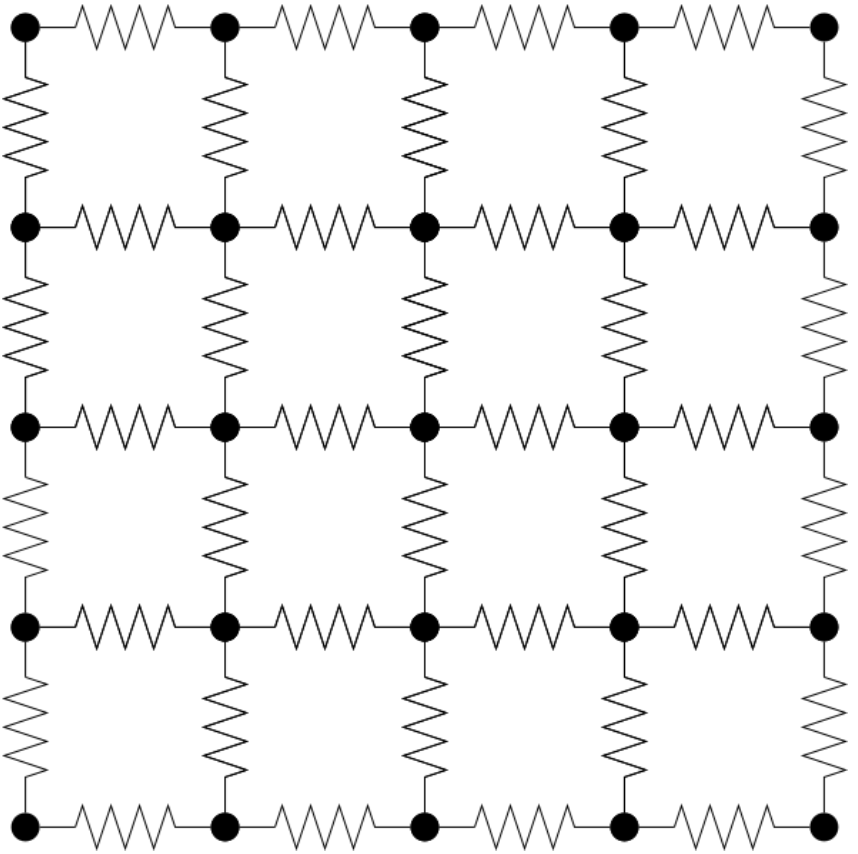
\includegraphics[width=\textwidth]{Ressort1.png} 
        \caption{Réseau de ressorts régulier}
        \label{fig:Ressort1}
    \end{subfigure}
    \hspace*{30pt}
    \begin{subfigure}[b]{0.3\textwidth}
        \centering
        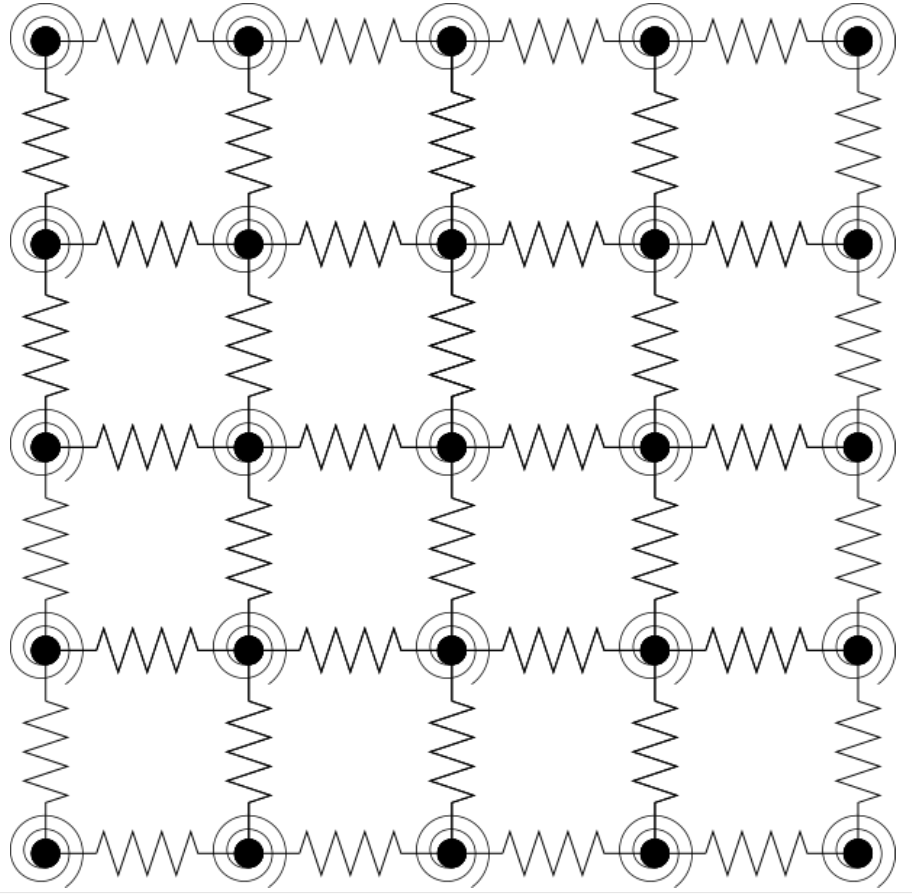
\includegraphics[width=\textwidth]{Ressort2.png} 
        \caption{Réseau de ressorts régulier avec torsion}
        \label{fig:Ressort2}
    \end{subfigure}
       \caption{Réseau de ressort considéré durant cette étude.}
       \label{fig:Reseau}
\end{figure}

Ensuite, \citeauthor{balasoiu2020halthesis} considère la suite $\tau_n$ de réseau défini, comme aux paragraphes précédents par 
$$
\tau_{n,0} = \Omega \cap \frac{1}{n} \mathbb{Z}^2 \,.
$$
On rappelle que $k_1$, $k_2$ représentent les constantes de raideurs des ressorts sur les arrêtes du réseau dans les deux directions de $\Omega$, et $G$ la constante de torsion des ressorts aux n\oe{}uds. Sur le maillage $\tau_n$, après définition des énergies redimensionnées élastiques de traction $R_n$, et de torsion $T_n$, \parencite[p.91]{balasoiu2020halthesis} montre les théorèmes suivants. 

\begin{theorem}[$\Gamma$-convergence]
    \label{theo:gammaconv}
    La suite d'énergie redimensionnée $(E_n)_{n\in\mathbb{N}}$ $\Gamma$-converge, pour la topologie faible de $H^1(\Omega, \mathbb{R}^2)$, vers la fonctionnelle limite :
    \begin{align*}
        \eel : H^1(\Omega, \mathbb{R}^2) &\rightarrow \mathbb{R} \\
        &u \mapsto \frac{1}{2} \int_{\Omega} C_h e(u):e(u) \diff x \,,
    \end{align*}
    avec $C_h$ le tenseur de rigidité du matériau homogénéisé, qui vérifie :
    $$
    C_{h,ijkl}M:M = k_1 M^2_{1,1} + k_2 M^2_{2,2} + 16G(M_{1,2} + M_{2,1})^2 \,,
    $$
    De plus, ce tenseur est celui d’un matériau élastique homogène et isotrope si et seulement si l’on a $k_1 = k_2 = k = 8G$. Dans ce cas, on a :
    $$
    \eel(u) = \frac{1}{2} \int_{\Omega} K_{\lambda, \mu}e(u) : e(u) \diff x \,,
    $$
    avec :
    $\lambda = 0$, et $\mu = \frac{k}{2}$.
\end{theorem}


\begin{theorem}[Équi-coercivité]
    Soit $(\tau_n)_{n\in\mathbb{N}}$ une suite de maillages du plan, et $(u_n) \in \mathbb{N}$ une suite de déplacements admissibles de $H^1(\Omega, \mathbb{R}^2)$, i.e. vérifiant :
    $$
        \forall n \in \mathbb{N}, \quad u_n \in \wadm (\tau_n, \mathbb{R}^2) \,.
    $$
    On suppose de plus que cette suite de déplacement est bornée pour l’énergie :
    $$
    \exists C > 0 , \forall n \in \mathbb{N}, \quad E_{n}(u_n) \leq C \,.
    $$
    Alors la suite $(u_n)_{n \in \mathbb{N}}$ est bornée dans $H^1(\Omega, \mathbb{R}^2)$.
\end{theorem}

Le \cref{theo:gammaconv} permet de constater que le tenseur de rigidité obtenu, lorsqu’il est isotrope, a un coefficient de Poisson nul\footnote{Cela correspond par exemple à un étirement longitudinal du réseau de ressorts, sans effet (amincissement ou épaississement) sur la section transversale.}. \citeauthor{balasoiu2020halthesis} a donc proposé un calcul formel de la limite simple de la suite d’énergies discrètes dans le cas ou le réseau de ressorts serait stochastique, de loi isotrope. En particulier, il trouve dans ce cas un coefficient de Poisson fixe de $1/4$.




\subsection{Un processus stochastique de maillages isotropes} 

\textit{Le résumé du chapitre écrit dans \parencite[p.136]{balasoiu2020halthesis} est le suivant. Ce chpitre fait appel à des outils fin de probabilé conditionnelle et de processus stochastiques, telles que \textbf{mesure et formules de Campbell}, \textbf{distribution de Palm}, etc. }

Dans ce chapitre, \citeauthor{balasoiu2020halthesis} a construit un processus stochastique de maillage, qui à chaque tirage associe un maillage de Delaunay. il a également donné plusieurs formules de calcul, les deux formules de Campbell ainsi que la formule de Slivnyak-Mecke, qui permettent de calculer l’espérance d’une variable aléatoire qui s’écrit comme la somme d’une fonction en chaque point du maillage. Ces formules nous se montrerons très utiles pour le calcul de
l’énergie élastique d’un réseau de ressorts basé sur ce processus de maillage.

Les maillages construits suivent une loi isotrope. En moyenne sur les tirages, toutes les directions des arrêtes sont donc équitablement représentées. Un théorème ergodique permet de transférer cette isotropie moyenne en isotropie presque sure si l’on dilate le maillage, autrement dit si on le regarde de suffisamment loin.

\citeauthor{balasoiu2020halthesis} montre aussi que, si l’on dilate le processus de Poisson-Delaunay initial et qu’on en restreint les réalisations à un domaine du plan, nous obtenons une suite de processus stochastiques dont les réalisations convergent presque sûrement vers le domaine fixé. Nous avons également donné un contrôle asymptotique de la taille minimale des mailles
obtenues dans cette suite de processus de maillages. Ce contrôle nous sera utile dans le chapitre suivant, pour calibrer le redimensionnement utilisé pour traduire l’hypothèse des petits déplacements sur le réseau de ressorts.



\textit{SIMULATION D'UN PROCESSUS DE POISSON: https://hpaulkeeler.com/poisson-point-process-simulation/}


La notions de processus poinctuel est un outil qui peut permettre de construire un ensemble de points dénombrable, sans point d'accumulation. \citeauthor{balasoiu2020halthesis} définit un \textbf{processus stochastique simple de $\mathbb{R}^d$} comme : une variable aléatoire $\Phi$ d’un espace de probabilités $(\Omega, \mathcal{A}, \mathbb{P})$ dans l’espace $(\mathfrak{N}, \mathcal{N})$. Elle induit une loi de probabilité $\mathbb{P}_\Phi$ sur $(\mathfrak{N}, \mathcal{N})$ : l’espace $(\mathfrak{N}, \mathcal{N}, \mathbb{P}_\Phi)$ est un espace de probabilités. Dans cette définition, nous avons:
\begin{itemize}
    \item $\mathfrak{N}$ est ensemble des parties localement finies de $\mathbb{R}^d$. Autrement dit, il s'agit de l'ensemble des motifs de points de $\mathbb{R}^d$;
    \item $\mathcal{N}$ est la plus petite tribu (sur $\mathfrak{N}$) qui rende mesurable les applications qui comptent le nombre de points du processus. 
\end{itemize}


\textit{Ci-dessous, QUELQUES EXMAPLES DE PROCESSUS STOHASTIQUES.}
 


\subsection{Étude asymptotique d’un réseau de ressorts isotrope} 

\textit{IMAGE D'UN RESSORT TRIANGULAIRE fig 5.1} \\
\textit{REECRIRE LE RESUME, ET LES DEUX THEOREMES QUI SONT MONTRÉS DANS CE CHAPITRE}



\subsection{Résultat de quasi-staticité à grande raideur} 

Ce chapitre propose un résultat de quasi-staticité d’un réseau de ressorts percuté par un objet ponctuel lorsque la raideur du système et sa masse totale tendent vers l’infini. Lors de la collision de floes de glaces, la vitesse relative des floes (de l’ordre de grandeur de la dizaine de centimètres par seconde, voir [RWMB09]) est bien inférieure à la vitesse de propagation des ondes élastiques dans la glace (de l’ordre de grandeur de 1800 mètres par seconde pour les ondes de cisaillement, voir [Mar+19]). \citeauthor{balasoiu2020halthesis} montrons que, lors de la percussion d’un réseau masse-ressort par un objet solide, les effets dynamiques disparaissent lorsque la raideur des ressorts tend vers l’infini. Autrement dit, nous montrons que le réseau limite, de raideur infinie, est à chaque instant dans un état d’équilibre. Plus précisément, nous observerons que le système différentiel qui modélise la percussion s’écrit comme le couplage de deux sous-systèmes. Le premier, dit \textbf{système intérieur} (SI), est à évolution rapide et modélise la propagation des ondes élastiques dans le système masse-ressort. Le second, dit \textbf{système extérieur} (SE), est à évolution lente et modélise la pénétration de l’objet solide dans le système masse-ressorts.

On étudie le phénomène de percussion d’un système masse-ressort de n + 1 particules, chacune de masse $m$, par un objet ponctuel $P$ de masse $M$. Le système masse-ressort utilisé est de constante de raideur $k>0$, et de constante de viscosité $\mu>0$. Soit $\tau \in \mathcal{T} (\Rdeux)$ une triangulation compacte et connexe du plan. En chaque noeud $q \in \tau_0$, on place une masse ponctuelle $m$ (voir \cref{fig:masseressort}). Sur chaque arrête $\omega \in \tau_1$ de $\tau$, on place en parallèle :
\begin{enumerate}
    \item un ressort de longueur à l’équilibre $\omega$ et de raideur $k$,\
    \item un dissipateur visqueux, de viscosité $\mu$.
\end{enumerate}
\begin{figure}[!h]
    \centering
    \frame{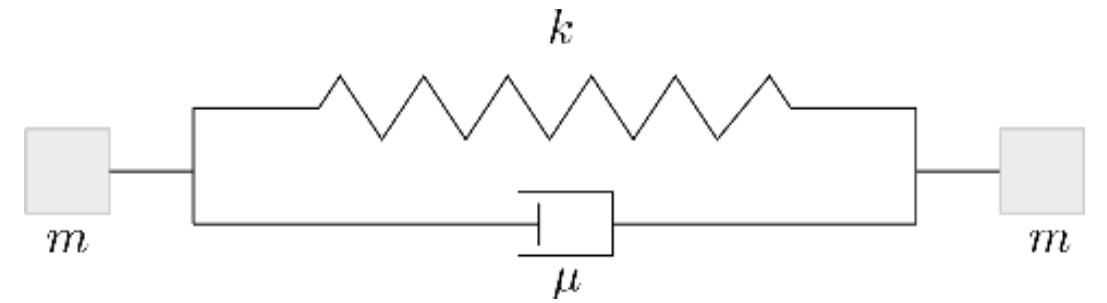
\includegraphics[width=0.5\textwidth]{MasseRessort.png}}
    \caption{Système élémentaire masse-ressort utilisé.}
    \label{fig:masseressort}
\end{figure}
On suppose qu’à l’instant $t = 0$, le système masse-ressorts est à l’équilibre, et qu’il est percuté par la masse ponctuelle $P$ au point $q_0 \in \partial\tau_0$. On note $v_0$ la vitesse du point $P$ lors
de la collision. On suppose également que le système $\{q0, P\}$ \textbf{devient inséparable}, de masse $m + M$.
Sur le maillage $\tau$ , on note $\tau_0$ l’ensemble des noeuds du système. On a donc :
$$\tau_0 = \{q_0, . . . , q_n \} \,,$$
où les $q_i$ sont les coordonnées des masses. On rappelle que le système est à l’équilibre au temps $t = 0$. On note $a, b \in \mathcal{M}_{2,n+1} (\Run)$ les vecteurs de positions et vitesses initiales définis
par :
$$
\begin{cases}
    a = (q_0(0), \ldots, q_n(0)) \,, \\
    b = (v_0,0,\ldots,0) \,.
\end{cases}
$$
On note de plus $C \in \mathcal{M}_{n+1}(\Run)$ la matrice de connectivité :
$$
∀0 \leq i < j \leq n + 1, C_{i,j} = C_{j,i} =
\begin{cases}
    1 si q_i \in \mathcal{V}(q_j) \,,
    0 sinon,
\end{cases}
$$
où $\mathcal{V}(q)$ désigne l’ensemble des voisins de la particule $q \in \tau_0$. On note encore $L_{ij} \in \mathcal{M}_{n+1} (\Run)$ la matrice de longueurs à l’équilibre dont l’expression est déduite de $τ_0$; et $u_{ij}$ le vecteur unitaire (s'il existe) dans la direction de l'arete entre $q_i$ et $q_j$. On obtient le système différentiel suivant en appliquant l'équation d'Euler-Newton sur les moments linéaires, et en exprimant la force de frotement du dispositif visqueux en fonction de $\dot q$ :
\begin{align} \tag{$E$} \label{eq:e}
\begin{dcases}
    \bvec{\ddot{q}}_0 = \sum_{j=0}^{n}C_{0j} \left[  \frac{k}{M+m} \left( \Vert \bvec{q}_j - \bvec{q}_0 \Vert - L_{0j} \right) \bvec{u}_{0j} -\frac{\mu}{M+m} \left\langle \bvec{\dot{q}}_j - \bvec{\dot{q}}_0\,, \bvec{u}_{0j}  \right\rangle  \bvec{u}_{0j}  \right] \,, &\qquad \text{(SE)} \\
    \bvec{\ddot{q}}_i = \sum_{j=0}^{n}C_{ij} \left[  \frac{k}{m} \left( \Vert \bvec{q}_j - \bvec{q}_i \Vert - L_{ij} \right) \bvec{u}_{ij} -\frac{\mu}{m} \left\langle \bvec{\dot{q}}_j - \bvec{\dot{q}}_i\,, \bvec{u}_{ij}  \right\rangle  \bvec{u}_{ij}  \right] \,, \quad \forall 1 \leq i \leq n \,. &\qquad \text{(SI)}
\end{dcases}
\end{align}

D'un point de vue énergétique, on a loi de conservation de l'énergie suivante:
\begin{align*}
    \eel(t) + E_{\text{c}}(t) + E_{\text{r}}(t) = E_0
\end{align*}
où $\eel(t), E_{\text{c}}$, et $E_{\text{r}}$ désignent respectivement l'énergie élastique du système, l'énergie cinétique, et l'énergie disipée par les frotement visqueux \parencite[p.188]{balasoiu2020halthesis}. $E_0$ désigne l'énergie intiale du système donnée par 
$$
E_0 = \frac{1}{2}(M+m)\Vert \bvec{v}_0 \Vert^2 \,.
$$
Sous ces hypothèses et ces définitions, \citeauthor{balasoiu2020halthesis} obtient le théorème d'existence globale suivant.
\begin{theorem}[Existence d'une solution globale] \label{th:solglob}
    On suppose que les conditions initiales adjointes au système \cref{eq:e} vérifient la condition énergétique :
    $$
    E_0 < \frac{k}{4} \left( \inf_{\omega \in \tau_1} \vert \omega \vert \right)^2 \,.
    $$
    Alors, le problème de Cauchy est bien posé\footnote{Le système est bien posé si deux particules voisines restent à une distance $c > 0$ l’une de l’autre.} et ses solutions sont globales.
\end{theorem}

Ensuite, afin d'obtenir un système a grande raideur et de supprimer la perturbations liées à la propagation des ondes élastiques, \citeauthor{balasoiu2020halthesis} introduit une dépendance en $\varepsilon$ des constantes physiques du système : $k_\varepsilon$ , $M_\varepsilon$ et $\mu_\varepsilon$. En posant 
$$
k_\varepsilon = \frac{k}{\varepsilon} \,, \quad M_\varepsilon = \frac{M}{\varepsilon^2} \, \quad \mu_\varepsilon = \frac{\mu}{\varepsilon} \,,
$$
le système masse-ressort se réecrit :
\begin{align} \tag{$E_{\varepsilon}$} \label{eq:eeps}
\begin{dcases}
    \bvec{\ddot{q}}_0 = \sum_{j=0}^{n}C_{0j} \left[  \frac{k}{M+\varepsilon^2 m} \left( \Vert \bvec{q}_j - \bvec{q}_0 \Vert - L_{0j} \right) \bvec{u}_{0j} - \varepsilon\frac{\mu}{M+\varepsilon^2 m} \left\langle \bvec{\dot{q}}_j - \bvec{\dot{q}}_0\,, \bvec{u}_{0j}  \right\rangle  \bvec{u}_{0j}  \right] \,, \\
    \varepsilon^2 \bvec{\ddot{q}}_i = \sum_{j=0}^{n}C_{ij} \left[  \frac{k}{m} \left( \Vert \bvec{q}_j - \bvec{q}_i \Vert - L_{ij} \right) \bvec{u}_{ij} - \varepsilon \frac{\mu}{m} \left\langle \bvec{\dot{q}}_j - \bvec{\dot{q}}_i\,, \bvec{u}_{ij}  \right\rangle  \bvec{u}_{ij}  \right] \,, \quad \forall 1 \leq i \leq n \,. 
\end{dcases}
\end{align}
On écrit également le système limite :
\begin{align} \tag{$E_{lim}$} \label{eq:elim}
\begin{dcases}
    \bvec{\ddot{q}}_0 = \sum_{j=0}^{n}C_{0j}  \frac{k}{M} \left( \Vert \bvec{q}_j - \bvec{q}_0 \Vert - L_{0j} \right) \bvec{u}_{0j}  \\
    \bvec{0} = \sum_{j=0}^{n}C_{ij} \frac{k}{m} \left( \Vert \bvec{q}_j - \bvec{q}_i \Vert - L_{ij} \right) \bvec{u}_{ij} \,, \quad \forall 1 \leq i \leq n \,.
\end{dcases}
\end{align}
Ce problème est un problème de perturbation singulière, pour lequel \citeauthor{balasoiu2020halthesis} prouve le théorème de limite quasi-statique ci-bas (en se servant principalement du théorème classique de A.N.Tikhonov [Tik52 ; Hop66]).
\begin{theorem}[Limite quasi-statique]
    Les solutions $ \bvec q_\varepsilon$ et $\bvec q$ respectivement des systèmes perturbé \cref{eq:eeps} et limite \cref{eq:elim} munis des conditions initales\footnote{Des conditions initiales satisfaisant le \cref{th:solglob}.} existent, sont uniques, et globales.
    De plus, on a :
    $$
    \lim_{\varepsilon \rightarrow 0} \bvec q_{\varepsilon}(t) = \bvec q(t) \,, \quad \forall t \in \mathbb{R}^+ \,.
    $$
\end{theorem}

Du point de vue numérique, les simulations ont permis de comprendre l’influence des différents paramètres physiques présents (masse des deux objets, raideur des ressorts, vitesse d’impact ...). De plus, le code Python et HTML/CSS developpé fournira une bonne base pour analyser la localisation des vecteurs propres du système dynamique et identifier ceux qui agissent sur un déplacement du bord. Le principal résultat numérique utilisé est le suivant. À $\varepsilon > 0$ fixé, on note $(\lambda_i (\varepsilon))i \in \{0,...,4n+3\}$ les valeurs propres de l’opérateur associé à la linéarisation du système \cref{eq:eeps} autour de sa position d’équilibre, et on les ordonne ainsi:
$$
0 \geq \mathfrak{R}(\lambda_8(\varepsilon)) \geq \mathfrak{R}(\lambda_9(\varepsilon)) \geq \ldots \geq \mathfrak{R}(\lambda_{4n+3}(\varepsilon)) \,.
$$
Nous définissons le saut spectral νε associé au système \cref{eq:eeps} de la manière suivante :
$$
\nu_{\varepsilon} = \frac{\mathfrak{R}(\lambda_{12}(\varepsilon))}{\mathfrak{R}(\lambda_{11}(\varepsilon))} \,.
$$
Ce saut représente l’écart entre les quatre premières valeurs propres non nulles du système, qui correspondent au système lent (SE), et la première valeur propre du système rapide (SI). Après avoir tracé le saut spectral $\nu_{\epsilon}$ pour différentes triangulations $\tau$ (cf. \cref{fig:res3} pour un exemple), \citeauthor{balasoiu2020halthesis} constate qu'il s'agit de droites dont la pentes ne dépendent ni du tirage, ni de l’intensité du processus de Poisson-Delaunay. Il propose donc l’expression suivante pour $\nu_{\varepsilon}$ :
$$
\ln(\nu_{\varepsilon}) = a_0(\tau) + \alpha \ln(\varepsilon) \,,
$$
avec $a_0 (\tau)$ une quantité qui dépend du maillage $\tau$, et $\alpha$ une constante universelle, indépen-
dante de $\tau$ et $\varepsilon$ numériquement estimée à la valeur :
$$\alpha = −2 \pm 10^{−3} \,.$$
La figure 6.4 ci-dessous ont été obtenue, pour un processus de Poisson-Delaunay d’intensité $500 000$, l’histogramme de la valeur de $a_0$ associée sur $1 000$ tirages (cf.\cref{fig:res2}).
\begin{figure}[H]
    \centering
    \begin{subfigure}{0.29\textwidth}
        \includegraphics[width=\textwidth]{Res3.png}
        \caption{Saut spectral en fonction de la perturbation, en échelle log-log, sur dix tirages d’un processus de Poisson-Delaunay d’intensité $1000$.}
        \label{fig:res3}
    \end{subfigure}
    \begin{subfigure}{0.3\textwidth}
        \includegraphics[width=\textwidth]{Res1.png}
        \caption{Histogrammes du paramètre $a_0$, sur $10 000$ tirages d’un processus de Poisson-Delaunay d’intensité $2500$.}
    \end{subfigure}
    \begin{subfigure}{0.3\textwidth}
        \includegraphics[width=\textwidth]{Res2.png}
        \caption{Histogramme du paramètre $a_0$ sur $1 000$ tirages d’un processus de Poisson-Delaunay d’intensité $500 000$}
        \label{fig:res2}
    \end{subfigure}
    % \decoRule
    \caption{Principaux résultats numériques obtenus \parencite[p.199]{balasoiu2020halthesis}.}
\end{figure}
\noindent Ces résultats semblent indiquer, à grande échelle au moins, que $a_0(\tau)$ prend ses valeurs entre $0.9$ et $2.5$. Nous observons également l’émergence de deux pics pour certaines
intensités. Il semblerait que le pic de valeur moyenne la plus faible gagne en fréquence de représentation, jusqu’à concentrer la quasi-totalité des cas pour l’intensité de $500 000$.












\subsection{Discussion}

Plusieurs hypothèses sont faites dans la thèse :
\begin{enumerate}
    \item Le modèle suppose que les floes sont d’épaisseur négligeable devant leur extension horizontale ; autrement dit, les déformations du floe de glace peuvent être étudiées en deux dimensions.
    \item Le modèle restreint l’ensemble des fractures admissibles à celui des segments de droites.
\end{enumerate}       %% État de l'art
% Chapter 4

\chapter{Travaux et apports} % 4th chapter title

\label{Chapter4} % For referencing the chapter elsewhere, use \ref{Chapter4} 


%----------------------------------------------------------------------------------------


\section{Les missions du poste}

\begin{itemize}
    \item L'état de l'art de la partie précédente fait partie des missions.
    \item Modélisation
    \item Simulation
\end{itemize}

Nous souhaitons étudier le comportement mécanique d'un floe après collision avec un autre floe. Les étapes de travail envisagées sont les suivantes:
\begin{enumerate}
    \item Ecire les systèmes differentiels pour les deux floes juste après le choc: pour l' instant on peut considérer que l'un des floes est immobile (celà revient au même si l'on exprimes les vitesses dans un repère lié à ce floe).
    \item On exprime l'EDO vérifiée par les solutions, c'est à dire $q$ pour le premier floes, et $p$ pour le second.
    \item On pourra ensuite simuler ces EDP limites et trouver les valeurs de $p$ et $q$. Autrement dit, on connait la position de chaque point du réseau au temps final.
    \item Si on connait $p$ et/ou $q$, on connait la condition de Dirichlet sur le floe concerné, et on peut ainsi exprimer le déplacement et la possible fracture du floe. 
\end{enumerate}




\section{Présentation des résultats obtenus}



\subsection{Modélisation générale du contact entre deux floes de glace}

Les floes de glace $\Omega_k$ et $\Omega_l$ sont modélisés par des systèmes masse-ressort (à grande raideur). Pour l'instant, nous considérons une moélisation simplifiée qui assimile un floe à un système de (trois) masses reliés par des ressorts (de constante de raideur $k$), et par des dispositifs visqueux de constante $\mu$.
Nous désignerons par $n+1$ le nombre total de noeuds du floe $\Omega_k$, chaque noeud ayant pour masse $m$. De facon similaire, on définit les constantes $k'$, $\mu'$, $n'+1$, $m'+1$ pour le floe $\Omega_l$. Les positions des noeds de $\Omega_k$ seront noté $(q_i)_{0\leq i\leq n}$, tandis que ceux de $\Omega_l$ seront notés $(p_i)_{0 \leq i\leq n'}$ (voir \cref{fig:contactmanuel}). 

\begin{figure}[!h]
    \centering
    \includegraphics[width=0.3\textwidth, angle=-90]{ContactManuel.jpg}
    \caption{Contact entre deux floes aux points $p_0 = q_0$.}
    \label{fig:contactmanuel}
\end{figure}

\noindent On définit la matrice de contact $C$...(voir these Dimitri), et $L_{0j}$.. et $u_{0j}$ ..

\noindent Comme présenté dans les travaux \parencite[p.186]{balasoiu2020halthesis}, le système différentiel qui modélise la percussion s’écrit comme le couplage de deux sous-systèmes. Le premier, dit système intérieur (SI), est à évolution rapide et modélise la propagation des ondes élastiques dans le système masse-ressort. Ici, nous dérivons facilement et réutilisont le SI comme présenté par \citeauthor{balasoiu2020halthesis}. Le second, dit système extérieur (SE), est à évolution lente et modélise la pénétration de l’objet solide dans le système masse-ressorts. Pour dériver le SE sur le floe $\Omega_k$, nous écrivons l'équation de Newton-Euler linéaire\footnote{La rotation du point matériel $q_0$ n'est pas prise en compte ici, d'où l'abscence de l'équation de Newton-Euler angulaire.} au point de contact $q_0$:
\begin{align}  \label{eq:SE}
m \ddot{\bvec{q}}_0 = \bvec{F}_0 + \bvec{F}^c_0 \,,
\end{align}
où 
\begin{align}  \label{eq:F0}
    \bvec{F}_0 = \sum_{j=0}^{n}C_{0j} \left[  \underbrace{k \left( \Vert \bvec{q}_j - \bvec{q}_0 \Vert - L_{0j} \right) \bvec{u}_{0j}}_{\text{Force de rappel}} - \underbrace{\mu \left\langle \bvec{\dot{q}}_j - \bvec{\dot{q}}_0\,, \bvec{u}_{0j}  \right\rangle  \bvec{u}_{0j}}_{\text{Force de dissipation}}  \right] \,,
\end{align}
représente la somme des forces de reaction et de disssipation exercées par le ressort et le dispositif visqueux sur le noeud $q_0$ ; et $\bvec{F}^c_0(t)$ la force de contact durant la collison entre les deux particules. En supposnat qu'il existe un repère de contact $\mathcal{R}^c = \{ q_0, \bvec{n}, \bvec{t} \}$ associé au floe $\Omega_k$ (voir \cref{fig:contactmanuel}), on peut écrire, pour $(\lambda, \beta) \in \Rdeux$ :
\begin{align}  \label{eq:F0c}
    \bvec{F}_0^c = \lambda \bvec{n} + \beta \bvec{t} \,.
\end{align}
Le système intérieur (SE) s'obtient facilement en combinant les équations \cref{eq:SE,eq:F0,eq:F0c}. Le système intérieur (SI) s'obtient lui (pour les autres noeuds du réseau) en y supprimant la force de contact. On obtient au final:
\begin{align} \tag{$E$} \label{eq:e}
\begin{dcases}
    m \ddot{\bvec{q}}_0 = \bvec{F}_0 + \bvec{F}^c_0  \,, &\qquad \text{(SE)} \\
    m \ddot{\bvec{q}}_i = \bvec{F}_i   \,, \quad \quad \quad \forall 1 \leq i \leq n \,. &\qquad \text{(SI)}
\end{dcases}
\end{align}
En ce qui concerne le floe $\Omega_l$, nous procédons de facons similaire et appliqons la 3ème loi de Newton (action-réaction) pour obtenir le système:
\begin{align} \tag{$E'$} \label{eq:eprime}
\begin{dcases}
    m' \ddot{\bvec{p}}_0 = \bvec{F}^{'}_0 - \bvec{F}^c_0  \,, &\qquad \text{(SE)} \\
    m' \ddot{\bvec{p}}_i = \bvec{F}^{'}_i   \,, \quad \quad \quad \forall 1 \leq i \leq n' \,, &\qquad \text{(SI)}
\end{dcases}
\end{align}
où $(\bvec{F}^{'}_i)_{0 \leq i \leq n'}$ sont définis de facon similaire à $\bvec{F}_0$ (voir \cref{eq:F0}).

Ensuite, il nous faut introduire des conditions portant sur la conservation de l'énergie, et la condition de non-interpénétration de Signorini\dots



\subsection{Modélisation et simulation 1D}



\subsubsection{Collision parfaitement inélastique avec un floe encastré à l'instant initial}

Nous effectuons ici une modélisation 1D de notre problème. Un floe est modélisé par un système masse-ressort de deux nœuds. Le floe 1 est immobilisé face au mur, et le floe 2 approche à la vitesse $\bvec{v}_0$. On identifie les nœuds $q_0$ et $p_0$ de la section précédente à leur masses respectives $m$ et $m'$ (voir \cref{fig:contact1d}).
\begin{figure}[!h]
    \centering
    \frame{\includegraphics[width=0.8\textwidth]{Percussion1D-Systeme}}
    \caption{Contact 1D parfaitement inélastique entre deux floes. Le floe percuté étant immobile et coincé au mur avant le choc.}
    \label{fig:contact1d}
\end{figure}

\noindent On suppose que durant la dynamique non régulière, les masses $m$ et $m'$ en contact forment une seule masse\footnote{Cette simplification a pour principal avantage de supprimer le traitement de la force de contact entre les deux masses.}
$m+m'$ dont
le déplacement est donné par la variable $x_1(t)$. Le déplacement de la masse $m'$ à l'autre bout du floe percuteur est nommé
$x_2(t)$. La masse $m$ qui est fixée au mur ne sera pas étudiée ici. Nous faisons à présent le bilan des forces qui
s'exercent ces
deux masses.
\begin{figure}[!h]
     \begin{subfigure}[b]{0.4\textwidth}
         \centering
         \frame{\includegraphics[width=\textwidth]{Percussion1D-Masse1}}
         \caption{Sur $m+m'$.}
         \label{fig:bilan11}
     \end{subfigure}
%     \hfill
     \begin{subfigure}[b]{0.3\textwidth}
         \centering
         \frame{\includegraphics[width=\textwidth]{Percussion1D-Masse2}}
         \caption{Sur $m'$.}
         \label{fig:bilan12}
     \end{subfigure}
        \caption{Bilan des forces appliquée sur les noeuds du système. Les valeurs indiquées sont les intensitées
            (positives) des forces durant une phase imaginée de compression des ressorts ($\bvec{v}_0 <0$ et donc
            $x_1 <0$). Pour obtenir l'intesité de la force de rappel du ressort $k'$, on peut imaginer $x_1$ imobile
            (on aura $x_2 < 0$, d'où $x_1 - x_2 > 0$) (voir \parencite{homodeling}).}
        \label{fig:bilan}
\end{figure}

\noindent En orientant convenablement le système (voir \cref{fig:contact1d}), on applique la loi de Newton-Euler linéaire
pour obtenir le système suivant et ses conditions initiales \footnote{J'ai des doutes sur cette condition
initiale. La vitesse initiale de $x_1$ est-elle vraiment nulle?}:
\begin{align}
    \begin{dcases}
    (m+m')\ddot x_1 = -kx_1 - \mu \dot x_1 + k'(x_2 - x_1) + \mu'(\dot x_2 - \dot x_1) \\
        m' \ddot x_2 =  -k'(x_2 - x_1) - \mu'(\dot x_2 - \dot x_1) 
    \end{dcases}
\end{align}
À l'instant initial $t_0$, on a le système suivant
\begin{align} \label{eq:percussion1d}
    \begin{dcases}
    (x_1(t_0), x_2(t_0)) = (0,0) \\
    (\dot x_1(t_0), \dot x_2(t_0)) = (0,-v_0)
    \end{dcases}
\end{align}
En posant $X = (x_1, x_2)^T \in \mathbb{R}^2$, l' \cref{eq:percussion1d} devient
\begin{align}
    \underbrace{\mymat{m+m'}{0}{0}{m'}}_{A} \myvec{\ddot{x}_1}{\ddot{x}_2} = \underbrace{\mymat{-\mu -
    \mu^\prime}{\mu'}{\mu'}{-\mu'}}_{B}
    \myvec{\dot{x}_1}{\dot{x}_2} + \underbrace{\mymat{-k-k'}{k'}{k'}{-k'}}_{C} \myvec{x_1}{x_2} \,.
\end{align}
Puisque $m, m'\neq 0$, la matrice $A$ est inversible et on obtient au final le problème de Cauchy suivant:

\begin{align} \label{eq:percussion1d2}
    \begin{dcases}
        \ddot{X}(t) = B' \dot{X}(t) + C'X(t) \,, \\
        (X(t_0), \dot X (t_0)) = \left( \myvec{0}{0}, \myvec{0}{-v_0} \right) \,,
    \end{dcases}
\end{align}
avec $B' = A^{-1}B$ et $C' = A^{-1}C$.

\noindent Il s'agit la d'un système d'EDO du deuxième ordre à coefficients constants. Transformons le en un système du
premier ordre pour
une
résolution plus aisée. On pose donc $Y= (X, \dot X)^T = (x_1, x_2, \dot{x}_1, \dot{x}_2)^T \in \mathbb{R}^4$ et le
système
\ref{eq:percussion1d2}
devient
\begin{align} \label{eq:systeme1d}
    \begin{dcases}
        \dot{Y}(t)= E Y(t) \\
        Y_0 = Y(t_0) = (0,0,0,-v_0)^T
    \end{dcases}
\end{align}
avec la matrice par blocs \[ E = \mymat{0}{I_2}{C'}{B'} \,, \] où $I_2$ désigne la matrice identité de
$\mathbb{R}^{2\times2}$.

\noindent Avec $t_0= 0$, la solution de ce système d'EDO du premier ordre à coefficients constants est unique et est donnée par
\begin{align}
    Y(t) = \exp(tE)Y_0
\end{align}

La résolution numérique du système passe par le calcul de l'exponentielle de la matrice $E \in  \mathbb{R}^4$ (VOIR figure ci-bas et NOTEBBOK ) \ldots
\begin{figure}[!h]
    \centering
    \includegraphics[width=0.4\textwidth]{SimuPercussion1D.png}
    \caption{Simulation de la percussion 1D entre deux floes avec $m=1$, $m'=1$, $k=16$, $k'=5$, $\mu=6$,
        $\mu'=2$, $v_0=-1.0$, $t_{f}=32$. On observe effectivement le ralentissement du système et une convergence
        vers l'état d'équilibre $Y_{eq}= (0,0,0,0)$.}
    \label{fig:simucontact1d}
\end{figure}

\noindent Pour certaines valeurs (specifiquement de $\mu$ et $\mu'$), on constate que le système converge vers son état d'équilibre attendu $Y_{eq} = (0,0,0,0)$. Il nous reste dans cette section:
\begin{enumerate}
    \item Calculer analytiquement et numériquement tous les état d'équilibres $Y_{eq} \in \ker(E)$; distinguer les états stables des autres.
    \item Calculer analytiquement l'exponentielle de la matrice $E$, et donner l'expression de la solution; déduire la condition sur les parametres pour que le système converge vers l'état d'équilibre voulu.
\end{enumerate} 




\subsubsection{Collision parfaitement inélastique sans présence du mur}

Contrairement au cas étudié dans la section précédente, le mur est supprimé dans cette section. On obtient donc une troisième variable $x_3$ décrivant le comportement du noeud qui était rattaché au mur. La schéma régissant ce système est donnée à la \cref{fig:contact1d2}. Le bilan des forces appliquées aux noeuds est présenté à la \cref{fig:bilan2}.

\begin{figure}[!h]
    \centering
    \frame{\includegraphics[width=0.8\textwidth]{Percussion1D-Systeme-2}}
    \caption{Contact 1D parfaitement inélastique entre deux floes. Le floe percuté étant non immobile (et non coincé au mur) avant le choc. On représnte également les variables $x_1$, $x_2$, et $x_3$ décrivant les movements de chaque noeud.}
    \label{fig:contact1d2}
\end{figure}

\begin{figure}[!h]
    \begin{subfigure}[b]{0.25\textwidth}
        \centering
        \frame{\includegraphics[width=\textwidth]{Percussion1D2-Masse1.png}}
        \caption{Sur $m$.}
        \label{fig:bilan12}
    \end{subfigure}
%     \hfill
    \begin{subfigure}[b]{0.31\textwidth}
        \centering
        \frame{\includegraphics[width=\textwidth]{Percussion1D2-Masse2}}
        \caption{Sur $m+m'$.}
        \label{fig:bilan22}
    \end{subfigure}
%     \hfill
    \begin{subfigure}[b]{0.23\textwidth}
        \centering
        \frame{\includegraphics[width=\textwidth]{Percussion1D2-Masse3}}
        \caption{Sur $m'$.}
        \label{fig:bilan32}
    \end{subfigure}
       \caption{Bilan des forces appliquée sur les noeuds du système. On procède de facon similaire à \cref{fig:bilan} pour obtenir les sens et les intensités de ces forces.}
       \label{fig:bilan2}
\end{figure}

\noindent Comme précédement, nous appliqons les lois de Newton pour obtenir:
\begin{align}
    \begin{dcases}
    m\ddot x_1 = -k(x_1 - x_2) - \mu (\dot x_1 - \dot x_2) \,, \\
    (m+m')\ddot x_2 = k(x_1 - x_2) + \mu (\dot x_1 - \dot x_2) - k'(x_2 - x_3) - \mu'(\dot x_2 - \dot x_3) \,, \\
        m' \ddot x_3 =  k'(x_2 - x_3) + \mu'(\dot x_2 - \dot x_3) \,. 
    \end{dcases}
\end{align}
Sous forme matricielle, on a
\begin{align}
    \underbrace{\mybigmat{m}{0}{0}{0}{m+m'}{0}{0}{0}{m'}}_{A} \mybigvec{\ddot{x}_1}{\ddot{x}_2}{\ddot{x}_3} =  
    \underbrace{\mybigmat{-k}{k}{0}{k}{-k-k'}{k}{0}{k'}{-k'}}_{B} \mybigvec{x_1}{x_2}{x_3} + 
    \underbrace{\mybigmat{-\mu}{\mu}{0}{\mu}{-\mu-\mu'}{\mu'}{0}{\mu'}{-\mu'}}_{C} \mybigvec{\dot{x}_1}{\dot{x}_2}{\dot{x}_3} \,.
\end{align}
Puisque $m, m'\neq 0$, la matrice $A$ est inversible. En posant $X = (x_1, x_2, x_3)^T \in \mathbb{R}^3$, le système d'EDO revient à l' \cref{eq:percussion1d22} suivante:
\begin{align} \label{eq:percussion1d22}
        \ddot{X}(t) = B' X(t) + C'\dot{X}(t) \,, 
\end{align}
où $B' = A^{-1}B$ et $C' = A^{-1}C$. On pose ensuite $Y= (X, \dot X)^T \in \mathbb{R}^6$ et le système \cref{eq:percussion1d22} devient 
\begin{align} \label{eq:systeme1d2}
        \dot{Y}(t)= E Y(t)
\end{align}
avec $$ E = \mymat{0}{I_3}{B'}{C'} \,.$$.


Remarquons qu'en enlevant le mur à gauche du domaine (voir \cref{fig:contact1d}), le système est devenu isolé. Nous pouvons donc appliquer la conservation de la quantité de mouvement pour identifier la vitesse de l'ensemble $m+m'$ après collision et fixation de la masse $m'$ (à vitesse $\bvec{v}_0$) sur la masse $m$ (de vitesse nulle). Pour simplifier les calculs, nous considérons les floes comme des solides rigides. La vitesse de l'ensemble juste après collision est notée $v_f$, et les quantités de mouvement avant et après choc sont notées $P_{\text{avant}}$ et $P_{\text{après}}$. On a:
\begin{align*}
    & \quad P_{\text{avant}} = P_{\text{après}} \\
    \Rightarrow & \quad 2m \bvec{v}_0 + 2m'\bvec{v'}_0 = (2m + 2m') \bvec{v}_f \\
    \Rightarrow & \quad \bvec{v}_f = \frac{m \bvec{v}_0 + m'\bvec{v'}_0}{m+m'}
\end{align*} 

\noindent On introduit ces conditions initiales dans l'\cref{eq:systeme1d2} pour obtenir le système de Cauchy ci-bas. Le résulat de la simulation est présenté à la figure \cref{fig:simucontact1d2}. 
\begin{align} \label{eq:systeme1d3}
    \begin{dcases}
        \dot{Y}(t)= E Y(t) \,, \\
        Y(t_0) = Y_0 = -v_f(0,0,0,1,1,1) \,.        
    \end{dcases}
\end{align}

\begin{figure}[!h]
    \centering
    \includegraphics[width=0.6\textwidth]{SimuPercussion1D2.png}
    \caption{Simulation de la percussion 1D entre deux floes (sans présence du mur) avec $m=1$, $m'=1$, $k=3$, $k'=22$, $\mu=6$, $\mu'=2$, $v_0=-1.8$, $t_{f}=5$. On observe effectivement le ralentissement du système et une convergence vers l'état d'équilibre $Y_{eq}= (0,0,0,0,0,0)$.} 
    \label{fig:simucontact1d2}
\end{figure}






\subsubsection{Collision inélastique avec séparation des masses}

Reprennons le cas du contact 1D et étudions ce qui se passe durant l'intervale de temps $\tdelta = [tmoins, tplus]$ de la collision. Cette fois, pour étudier la dynamique non régulière, nous décidons de séparer les masses $m$ et $m'$ en contact (et ce même durant le contact). Le système résultant est très similaire aux deux cas traités précédemment (\cref{fig:contact1d,fig:contact1d2}), et nous le présentons à la \cref{fig:contact1d3} ci-bas, et son bilan de forces à la \cref{fig:bilan3}.

\begin{figure}[!h]
    \centering
    \frame{\includegraphics[width=0.8\textwidth]{Percussion1D-Systeme-3}}
    \caption{Contact 1D inélastique entre deux floes. Durant le choc, les noeuds $m$ et $m'$ en contact sont étudiés séparement. On représnte les variables $x_1$, $x_2$, $x_3$, et $x_4$ décrivant les movements de chaque noeud.}
    \label{fig:contact1d3}
\end{figure}


\begin{figure}[!h]
    \begin{subfigure}[b]{0.30\textwidth}
        \centering
        \frame{\includegraphics[width=\textwidth]{Percussion1D3-Masse1.png}}
        \caption{Sur $m$ de gauche ($x_1$).}
        \label{fig:bilan13}
    \end{subfigure}
%     \hfill
    \begin{subfigure}[b]{0.35\textwidth}
        \centering
        \frame{\includegraphics[width=\textwidth]{Percussion1D3-Masse2}}
        \caption{Sur $m$ de droite ($x_2$).}
        \label{fig:bilan23}
    \end{subfigure}
%     \hfill
    \begin{subfigure}[b]{0.35\textwidth}
        \centering
        \frame{\includegraphics[width=\textwidth]{Percussion1D3-Masse3}}
        \caption{Sur $m'$ de gauche ($x_3$).}
        \label{fig:bilan33}
    \end{subfigure}
%     \hfill
    \begin{subfigure}[b]{0.30\textwidth}
        \centering
        \frame{\includegraphics[width=\textwidth]{Percussion1D3-Masse4}}
        \caption{Sur $m'$ de droite ($x_4$).}
        \label{fig:bilan43}
    \end{subfigure}
       \caption{Bilan des forces appliquée sur les $4$ noeuds du système. On procède de facon similaire aux \cref{fig:bilan,fig:bilan2} pour obtenir les sens et les intensités de ces forces. $F_c$ représente la force de contact dont l'intensité est inconnue.}
       \label{fig:bilan3}
\end{figure}

\noindent Comme précédement, nous appliqons les lois de Newton pour obtenir:
\begin{align}
    \begin{dcases}
    m\ddot x_1 = -k(x_1 - x_2) - \mu (\dot x_1 - \dot x_2) \,, \\
    m\ddot x_2 = k(x_1 - x_2) + \mu (\dot x_1 - \dot x_2) - F_c \,, \\
    m'\ddot x_3 = - k'(x_3 - x_4) - \mu'(\dot x_3 - \dot x_4) + F_c \,, \\
        m' \ddot x_4 =  k'(x_3 - x_4) + \mu'(\dot x_3 - \dot x_4) \,. 
    \end{dcases}
\end{align}
On additionne membre à membre les équations régissant les mouvements de $x_2$ et $x_3$ pour éliminer la force de contact $F_c$ et obtenir le système:
\begin{align}\label{eq:systeme3test}
    \begin{dcases}
    m\ddot x_1 = -k(x_1 - x_2) - \mu (\dot x_1 - \dot x_2) \,, \\
    m\ddot x_2 + m'\ddot x_3 = k(x_1 - x_2) + \mu (\dot x_1 - \dot x_2) - k'(x_3 - x_4) - \mu'(\dot x_3 - \dot x_4) \,, \\
        m' \ddot x_4 =  k'(x_3 - x_4) + \mu'(\dot x_3 - \dot x_4) \,. 
    \end{dcases}
\end{align}
Remarquons que ce système reviens au même systeme étudié dans la partie précédente en posant $x_2(t) = x_3(t) $ p.p. En effet, durant la phase de contact, les massess $m$ et $m'$ peuvent etrs étudiées comme une unique masse $m+m'$. La grosse diffculté qui ressort de cette modélisation est la définitions de la vitesse initiale de l'ensemble $m+m'$. Celà dit, nous cherchons à trouver les vitessses $\dot x_1(\tplus)$, $\dot x_2(\tplus)$, $\dot x_3(\tplus)$ et $\dot x_4(\tplus)$ immédiatemetn après la collision. De par la ressemblance de ce modèle avec celui de la section précédente (voir \cref{eq:systeme1d2}), nous réutilisons les quantités $\dot x_1$ et $\dot x_4$ données par ce système (l'\cref{eq:systeme1d2} dans lequel $x_2$ et $x_3$ sont confondus). On peut se permertre une telle approximation car $x_1$ et $x_4$ n'interviennent pas directemetn dans la collision. De plus, la quantité $k(x_1 - x_2) + \mu (\dot x_1 - \dot x_2) - k'(x_3 - x_4) - \mu'(\dot x_3 - \dot x_4)$
% \begin{align}
%     I = k(x_1 - x_2) + \mu (\dot x_1 - \dot x_2) - k'(x_3 - x_4) - \mu'(\dot x_3 - \dot x_4)    
% \end{align}
est aussi calculé suivant le modèle \cref{eq:systeme1d2} (voir l'article \parencite{tommasino2020effect} pour une modélisation similaire). Il ne nous reste véritablement que $2$ inconnue dans notre dynamique irrégulière.

\noindent Intégrons la deuxième équation de \ref{eq:systeme3test} entre les instants $\tmoins$ et $\tplus$. On obtient:
\begin{align}    \label{eq:debuteq1}
    \int_{\tmoins}^{\tplus} m\ddot x_2 + m'\ddot x_3 \diff t = \underbrace{\int_{\tmoins}^{\tplus} k(x_1 - x_2) + \mu (\dot x_1 - \dot x_2) - k'(x_3 - x_4) - \mu'(\dot x_3 - \dot x_4) \diff t}_{I} \,.
\end{align}
Afin d'éviter toute confusion, nous notons $v_0 = \dot{x}_2(\tmoins)$ et $v'_0 = \dot{x}_3(\tmoins)$ les vitesses des noeuds en contact avant collision, et $V_0 = \dot{x}_2(\tplus)$ et $V'_0 = \dot{x}_3(\tplus)$ les vitesses après contact. L'équation \cref{eq:debuteq1} devient donc:
\begin{align} \label{eq:crammer1}
    mV_0 + m'V'_0 = I + mv_0 + m'v'_0 \,.
\end{align}
À présent, nous pouvons étudier l'énergie cinétique du système à travers le coefficient de restitution $\varepsilon$ \footnote{Le coefficient de restitution est le même que celui utilisé dans la thèse \parencite{rabatel2015thesis}.}. On suppose (algébriquement) que les noeuds prennent des directions indiquées à la \cref{fig:contact1dapres}. 
\begin{figure}[!h]
    \centering
    \frame{\includegraphics[width=0.6\textwidth]{Percussion1D3-Apres.png}}
    \caption{Situation après contact 1D.}
    \label{fig:contact1dapres}
\end{figure}

\noindent On obtient l'\cref{eq:crammer2}
\begin{align} \label{eq:crammer2}
    - V_0 + V'_0 = \varepsilon (v_0 - v'_0) \,.
\end{align}
Le système de Cramer qui découle des \cref{eq:crammer1,eq:crammer2} permet d'obtenir les expressions:
\begin{align}
    V_0 = \frac{I + (m+\varepsilon m')v_0 + (1-\varepsilon)m'v'_0}{m+m'} \,, \quad V'_0 = \frac{I + (1-\varepsilon)mv_0 + (m'+\varepsilon m)v'_0}{m+m'} \,.
\end{align}




























% \section{Les apports du stage}

%\begin{itemize}
%    \item L' utilisation de TIKZ
%\end{itemize}       %% Travaux et apports
% % Chapter 5

\chapter{Problème 2D et percussion des floes de glace} % 5th chapter title

\label{Chapter5} % For referencing the chapter elsewhere, use \ref{Chapter5} 

%1----------------------------------------------------------------------------------------







\section{Présentation des travaux antérieurs}










% \subsection{Fracture liée un déplacement quasi-statique}

% \subsection{Trajectoire d'un floe percuté}










%2----------------------------------------------------------------------------------------

\section{Dévelopement d'un modèle de percussion}










% \subsection{Déplacement d'un floe isolé}

% Étudions le comportement d'un floe de glace 2D modélisé par un réseau de ressorts (3 ressort, 3 dispositif viseux, et 3 noeuds) (voir \cref{fig:deplacement2d}).
% \begin{figure}[!h]
%     \centering
%     \includegraphics[width=0.3\textwidth]{Deplacement2D-1.png}
%     \caption{Floe de glace 2D modélisé par un réseau de ressorts. Le floe est isolé de toutes forces extérieurs. Tous les neouds du réseau ont la même masse $m$, tous les ressorts on la même raideur $k$, et tous les dispositifs visquens ont le même coefficient $\mu$.}
%     \label{fig:deplacement2d}
% \end{figure}


% \noindent Comme nous l'avons présenté aux \cref{eq:F0,eq:e}, le système de la \cref{fig:deplacement2d} est régit par l' équation:
% \begin{align} \label{eq:eprime2}
%     \forall i \in \mathbb{Z}/3\mathbb{Z}, \quad m \ddot{\bvec{q}}_i = \sum_{j=i+1}^{i+2}C_{ij} \left[  k \left( \Vert \bvec{q}_j - \bvec{q}_i \Vert - L_{ij} \right) \bvec{u}_{ij} - \mu \left\langle \bvec{\dot{q}}_j - \bvec{\dot{q}}_i, \, \bvec{u}_{ij}  \right\rangle  \bvec{u}_{ij}  \right]  , 
% \end{align}
% où $L_{ij}$ représente la longeur au repos du ressort entre les noeuds $i$ et $j$, et $C_{ij}$ indique si les noeuds $i$ et $j$ sont connectés ou non (pour ce modèle 2D simple, $C_{ij} = 1 \, \forall 0 \leq i,j \leq 2$). Le vecteur unitaire $\bvec{u}_{ij}$ vaut:
% $$
% \bvec{u}_{ij} = \frac{\bvec{q}_j - \bvec{q}_i}{\Vert \bvec{q}_j - \bvec{q}_i \Vert}.
% $$


% \paragraph{Simulation par un schéma d'Euler explicite.}

% On discrétise par un schéma de différence finies avec $N+1$ pas de temps, et pour une temps de simulations $T$:
% $$
% \forall i \in \mathbb{Z}/3\mathbb{Z}, \, \forall n \in [\![ 0,N ]\!], \quad  t^n = n\Delta t = n\frac{T}{N}, \quad \bvec{q}_i(t^n) \approx \bvec{q}_i^n.
% $$
% L'\cref{eq:eprime2} devient:
% $$
% m\frac{\bvec{q}_{i}^{n+1}-2\bvec{q}_{i}^{n}+\bvec{q}_{i}^{n-1}}{\Delta t^2} = \sum_{j=i+1}^{i+2}C_{ij}\left[ k \left( \Vert \bvec{q}_j^n - \bvec{q}_i^n \Vert - L_{ij} \right) \bvec{u}_{ij} - \mu \left\langle \frac{\bvec{q}_{j}^{n}-\bvec{q}_{j}^{n-1}}{\Delta t} - \frac{\bvec{q}_{i}^{n}-\bvec{q}_{i}^{n-1}}{\Delta t}, \, \bvec{u}_{ij} \right\rangle  \bvec{u}_{ij}  \right],
% $$
% soit encore:
% \begin{align} \label{eq:systeme2D}
%     \bvec{q}_{i}^{n+1} = 2\bvec{q}_{i}^{n}-\bvec{q}_{i}^{n-1} + \frac{\Delta t^2}{m} \sum_{j=i+1}^{i+2}C_{ij}\left[ k \left( \Vert \bvec{q}_j^n - \bvec{q}_i^n \Vert - L_{ij} \right) \bvec{u}_{ij} - \frac{\mu}{\Delta t} \left\langle \bvec{q}_{j}^{n}-\bvec{q}_{j}^{n-1} - \bvec{q}_{i}^{n}+\bvec{q}_{i}^{n-1}, \, \bvec{u}_{ij} \right\rangle  \bvec{u}_{ij}  \right].
% \end{align}
% La simulation de ce modèle par un schéma d'Euler explicite à pas constant sur un intervalle de temps faible ($T = 4$) est présentée à la \cref{fig:PlotDeplacement2D1Conv}, ainsi que les positions des 2 noeuds au début et à la fin de la simulation. La simulation à la \cref{fig:PlotDeplacement2D1NonConv} permet d'observer le problème avec ce schéma ($T = 10$).


% \begin{figure}[!h]
%     \begin{subfigure}[b]{0.7\textwidth}
%         \centering
%         \includegraphics[width=\textwidth]{PlotDeplacement2D-1-Conv.png}
%         \caption{Simulation des positions des noeuds.}
%         \label{fig:dep}
%     \end{subfigure}
% %     \hfill
%     \begin{subfigure}[b]{0.7\textwidth}
%         \centering
%         \includegraphics[width=\textwidth]{PositionInitFinales.png}
%         \caption{Illustration des positions initiales et finales des neouds.}
%         \label{fig:pos}
%     \end{subfigure}
%     \caption{Simulation du système \ref{eq:systeme2D} par un schéma d'Euler explicite avec $T = 4$. La couleurs rouge repésente le noeud $\bvec{q}_1$, le vert le noeud $\bvec{q}_2$, le blue le $\bvec{q}_3$. Les paramètres utilisés ici sont les suivants: $m=6.2$, $k=23.3$, $\mu=3$; à l'instant initiale, les trois noeuds perturbés avec des vitesses d'intensité respectives $v_1=0.3$, $v_2=0.1$, et $v_3=0.1$. Par rapport à l'axe des abcisses, ces vitesses ont sont orintées respectivement de $\theta_1=180^\circ$, $\theta_2=270^\circ$, et $\theta_3=240^\circ$ (voir \texttt{code/simu2D/Deplacement2D-1.ipynb}).}
%     \label{fig:PlotDeplacement2D1Conv}
% \end{figure}


% \begin{figure}[!h]
%     \centering
%     \includegraphics[width=0.7\textwidth]{PlotDeplacement2D-1-NonConv.png}
%     \caption{Simulation du système \ref{eq:systeme2D} par un schéma d'Euler explicite avec $T = 10$. Cette figure utilise les même paramtètres que la \cref{fig:PlotDeplacement2D1Conv}. On observe ici une divergence totale du système.}
%     \label{fig:PlotDeplacement2D1NonConv}
% \end{figure}

% Les \cref{fig:PlotDeplacement2D1Conv,fig:PlotDeplacement2D1NonConv} permettent de constater que le schéma d'Euler explicite (peu importe son pas de temps), n'est pas adapté à ce problème. Nous étudierons donc d'autres alternatives. 

 
% \paragraph{Simulation à l'aide des fonction de la librarie Scipy.} À travers ses fonction telle que \texttt{odeint} et $\verb|solve_ivp|$, \texttt{Scipy} offre une solution robuste et élégante pour simuler les systèmes d'ODE de la forme $Y' = AY$.


 




% \subsection{Modélisation du contact entre deux floes}

% Les floes de glace $\Omega_k$ et $\Omega_l$ sont modélisés par des systèmes masse-ressort (à grande raideur). Pour l'instant, nous considérons une moélisation simplifiée qui assimile un floe à un système de (trois) masses reliés par des ressorts (de constante de raideur $k$), et par des dispositifs visqueux de constante $\mu$.
% Nous désignerons par $n+1$ le nombre total de noeuds du floe $\Omega_k$, chaque noeud ayant pour masse $m$. De facon similaire, on définit les constantes $k'$, $\mu'$, $n'+1$, $m'+1$ pour le floe $\Omega_l$. Les positions des noeds de $\Omega_k$ seront noté $(q_i)_{0\leq i\leq n}$, tandis que ceux de $\Omega_l$ seront notés $(p_i)_{0 \leq i\leq n'}$ (voir \cref{fig:contactmanuel}). 

% \begin{figure}[!h]
%     \centering
%     \includegraphics[width=0.3\textwidth, angle=-90]{ContactManuel.jpg}
%     \caption{Contact entre deux floes aux points $p_0 = q_0$.}
%     \label{fig:contactmanuel}
% \end{figure}

% \noindent On définit la matrice de contact $C$...(voir these Dimitri), et $L_{0j}$.. et $u_{0j}$ ..

% \noindent Comme présenté dans les travaux \parencite[p.186]{balasoiu2020halthesis}, le système différentiel qui modélise la percussion s’écrit comme le couplage de deux sous-systèmes. Le premier, dit système intérieur (SI), est à évolution rapide et modélise la propagation des ondes élastiques dans le système masse-ressort. Ici, nous dérivons facilement et réutilisont le SI comme présenté par \citeauthor{balasoiu2020halthesis}. Le second, dit système extérieur (SE), est à évolution lente et modélise la pénétration de l’objet solide dans le système masse-ressorts. Pour dériver le SE sur le floe $\Omega_k$, nous écrivons l'équation de Newton-Euler linéaire\footnote{La rotation du point matériel $q_0$ n'est pas prise en compte ici, d'où l'abscence de l'équation de Newton-Euler angulaire.} au point de contact $q_0$:
% \begin{align}  \label{eq:SE}
% m \ddot{\bvec{q}}_0 = \bvec{F}_0 + \bvec{F}^c_0 \,,
% \end{align}
% où 
% \begin{align}  \label{eq:F0}
%     \bvec{F}_0 = \sum_{j=0}^{n}C_{0j} \left[  \underbrace{k \left( \Vert \bvec{q}_j - \bvec{q}_0 \Vert - L_{0j} \right) \bvec{u}_{0j}}_{\text{Force de rappel}} - \underbrace{\mu \left\langle \bvec{\dot{q}}_j - \bvec{\dot{q}}_0\,, \bvec{u}_{0j}  \right\rangle  \bvec{u}_{0j}}_{\text{Force de dissipation}}  \right] \,,
% \end{align}
% représente la somme des forces de reaction et de disssipation exercées par le ressort et le dispositif visqueux sur le noeud $q_0$ ; et $\bvec{F}^c_0(t)$ la force de contact durant la collison entre les deux particules. En supposnat qu'il existe un repère de contact $\mathcal{R}^c = \{ q_0, \bvec{n}, \bvec{t} \}$ associé au floe $\Omega_k$ (voir \cref{fig:contactmanuel}), on peut écrire, pour $(\lambda, \beta) \in \Rdeux$ :
% \begin{align}  \label{eq:F0c}
%     \bvec{F}_0^c = \lambda \bvec{n} + \beta \bvec{t} \,.
% \end{align}
% Le système intérieur (SE) s'obtient facilement en combinant les équations \cref{eq:SE,eq:F0,eq:F0c}. Le système intérieur (SI) s'obtient lui (pour les autres noeuds du réseau) en y supprimant la force de contact. On obtient au final:
% \begin{align} \tag{$E$} \label{eq:e}
% \begin{dcases}
%     m \ddot{\bvec{q}}_0 = \bvec{F}_0 + \bvec{F}^c_0  \,, &\qquad \text{(SE)} \\
%     m \ddot{\bvec{q}}_i = \bvec{F}_i   \,, \quad \quad \quad \forall 1 \leq i \leq n \,. &\qquad \text{(SI)}
% \end{dcases}
% \end{align}
% En ce qui concerne le floe $\Omega_l$, nous procédons de facons similaire et appliqons la 3ème loi de Newton (action-réaction) pour obtenir le système:
% \begin{align} \tag{$E'$} \label{eq:eprime}
% \begin{dcases}
%     m' \ddot{\bvec{p}}_0 = \bvec{F}^{'}_0 - \bvec{F}^c_0  \,, &\qquad \text{(SE)} \\
%     m' \ddot{\bvec{p}}_i = \bvec{F}^{'}_i   \,, \quad \quad \quad \forall 1 \leq i \leq n' \,, &\qquad \text{(SI)}
% \end{dcases}
% \end{align}
% où $(\bvec{F}^{'}_i)_{0 \leq i \leq n'}$ sont définis de facon similaire à $\bvec{F}_0$ (voir \cref{eq:F0}):
% \begin{align}
%     \bvec{F}'_i = \sum_{j=i}^{n'}C_{ij} \left[ k' \left( \Vert \bvec{p}_j - \bvec{p}_i \Vert - L'_{ij} \right) \bvec{u'}_{ij} - \mu' \left\langle \bvec{\dot{p}}_j - \bvec{\dot{p}}_i\,, \bvec{u}'_{ij}  \right\rangle  \bvec{u}'_{ij}  \right] \,.
% \end{align}

% \noindent Ensuite, on additionne membre à membre les équations des systèmes extérieurs (SE) de \cref{eq:e,eq:eprime} pour éliminer la force de contact. On obtient:
% \begin{align}
% m \ddot{\bvec{q}}_0 + m' \ddot{\bvec{p}}_0 = \bvec{F}_0 + \bvec{F}^{'}_0 \,.
% \end{align}
% Remarquons que les positions relatives des noeuds $\bvec{q}_0$ et $\bvec{p}_0$ restent inchangées durant la collision. A l'instant initial, on note donc $\Delta_0 = \bvec{q}_0(0) - \bvec{p}_0(0)$, et $\bvec{\dot q}_0(0) = \bvec{\dot p}_0(0)$ ; idéalement, nous voudrions que:
% \begin{align}
% \forall t \in \mathbb{R}^+ \,, \quad \bvec{q}_0(t) - \bvec{p}_0(t) = \Delta_0\,.
% \end{align}
% Pour satifaire cette condition, nous exhibons $n+n'+2$ équations nécessaire pour que notre problème de percussion soit bien posé. Elles sont :
% \begin{align} \tag{$\mathcal{P}$} \label{eq:problemeP}
% \begin{dcases}
%     (m+m') \ddot{\bvec{q}}_0  = \bvec{F}_0 + \bvec{F}^{'}_0  \,, &\qquad \text{(SE)} \\
%     \ddot{\bvec{p}}_0 = \ddot{\bvec{q}}_0 \,, &\qquad \text{(SE)} \\
%     m \ddot{\bvec{q}}_i = \bvec{F}_i   \,, \quad \quad \quad \forall 1 \leq i \leq n \,. &\qquad \text{(SI)} \\
%     m' \ddot{\bvec{p}}_i = \bvec{F}^{'}_i   \,, \quad \quad \quad \forall 1 \leq i \leq n' \,, &\qquad \text{(SI)}
% \end{dcases}
% \end{align}

% Ensuite, il nous faut introduire des conditions portant sur la conservation de l'énergie, et la condition de non-interpénétration de Signorini\dots







%3----------------------------------------------------------------------------------------

\section{Présentation du code de calcul 1D}







%4----------------------------------------------------------------------------------------

\section{Résumé des résultats obtenus}

       %% Déroulement du stage
% % Chapter 6

\chapter{Conclusion} % 6th chapter title

\label{Chapter6} % For referencing the chapter elsewhere, use \ref{Chapter6} 

%----------------------------------------------------------------------------------------


Pour conclure, j'ai effectué mon stage de fin d'étude au Laboratoire Jacques-Louis Lions sous la supervision du professeur Stéphane Labbé. Durant six mois au sein de ce célèbre laboratoire de mathématiques appliquées, je me suis confronté au problème de la \emph{fracturation des floes de glace} dans un modèle granulaire. J'ai ainsi pu mettre en pratique mes connaissances en calcul scientifique, en analyse numérique, en EDP, en analyse fonctionnelle, et en développement Python (et bien d'autres) acquises durant ma formation de \href{https://www.unistra.fr/etudes/decouvrir-nos-formations/par-facultes-ecoles-instituts/sciences-technologies/ufr-de-mathematique-et-dinformatique/ufr-de-mathematique-et-dinformatique/cursus/ME195?cHash=3aa4f04702a03e944ed933056abe17f2}{CSMI}. 

À travers les objectifs secondaires que nous nous sommes fixés, j'ai pu comprendre le modèle de rupture de Griffith dans les milieux élastiques en assimilant des domaines clés de l'analyse fonctionnelle tels que la $\Gamma$-convergence, la résonance, et la probabilité; j'ai posé les bases du passage micro/macro du modèle élastique et j'ai développé plusieurs modèles de percussion (1D et 2D). J'ai acquis de l'expérience en programmation d’un modèle mathématique par différents schémas numériques, et en suivi de son intégration à un projet de développement logiciel. Sur un plan technique, j'ai maitrisé plusieurs outils informatiques tels que TikZ, Flask, Bokeh, et Symbolab.

Cela dit, il reste plusieurs travaux à effectuer pour conclure ce travail. Nous pouvons par exemple citer l'implémentation de la méthode du champ de phase dans le modèle 1D, l'implémentation de la fracture dans le problème 2D, le passage en dimension supérieure (2.5D ou 3D), l'optimisation du code, des tests de confirmation de l'approximation par réseaux de ressorts à grande raideur, et des tests de validation des modèles en laboratoire.

Fort de cette expérience et de ses enjeux cruciaux pour l'industrie et pour la planète, j'aimerais apporter ma contribution à la science à travers ce projet et d'autres similaires. Le projet \href{https://sasip-climate.github.io/}{SASIP} qui a fait de la compréhension du \emph{réchauffement climatique en zone polaire} sa mission phare est une initiative à soutenir et à répéter.       %% Conclusion

%----------------------------------------------------------------------------------------
%	THESIS CONTENT - APPENDICES
%----------------------------------------------------------------------------------------

% \appendix % Cue to tell LaTeX that the following "chapters" are Appendices

% Include the appendices of the thesis as separate files from the Appendices folder
% Uncomment the lines as you write the Appendices

% 
% Appendix A

\chapter{How to reproduce the results?} % Main appendix title

% 
% Appendix B

\chapter{Le schéma Symplectique} % Appendix B title

EXPLICATION DU MODULE SCIPY INTEGRATE

%\include{Appendices/AppendixC}

%----------------------------------------------------------------------------------------
%	BIBLIOGRAPHY
%----------------------------------------------------------------------------------------

\printbibliography[heading=bibintoc]

%----------------------------------------------------------------------------------------

\end{document}

